\documentclass[11pt,professionalfonts,aspectratio=169,handout]{beamer}

\usepackage{defense_packages}
%%%%%%%%%%%%%%%%%%%%%%%%%%%%%%%%
% CUSTOM MACROS
%%%%%%%%%%%%%%%%%%%%%%%%%%%%%%%%%%

\newcommand{\linearize}[3]{\ensuremath{\left. \frac{\partial #1}{\partial #2} \right|_{#3} \delta #2}}
\newcommand{\norm}[1]{\ensuremath{\left\| #1 \right\|}}
\newcommand{\abs}[1]{\ensuremath{\left| #1 \right|}}
\newcommand{\Real}[1]{\ensuremath{\Re \left\{ #1 \right\}}}
\newcommand{\bracket}[1]{\ensuremath{\left[ #1 \right]}}
\newcommand{\braces}[1]{\ensuremath{\left\{ #1 \right\}}}
\newcommand{\parenth}[1]{\ensuremath{\left( #1 \right)}}
\newcommand{\pair}[1]{\ensuremath{\langle #1 \rangle}}
\newcommand{\met}[1]{\ensuremath{\langle\langle #1 \rangle\rangle}}
\newcommand{\refeqn}[1]{(\ref{eqn:#1})}
\newcommand{\reffig}[1]{Fig.~\ref{fig:#1}}
\newcommand{\tr}[1]{\mathrm{tr}\ensuremath{\negthickspace\bracket{#1}}}
\newcommand{\trs}[1]{\mathrm{tr}\ensuremath{[#1]}}
\newcommand{\deriv}[2]{\ensuremath{\frac{\partial #1}{\partial #2}}}
\newcommand{\dderiv}[2]{\ensuremath{\frac{\partial^2 #1}{\partial^2 #2}}}
\newcommand{\dderivc}[3]{\ensuremath{\frac{\partial #1}{\partial #2 \partial #3}}}
\newcommand{\diff}[2]{\ensuremath{\frac{d #1}{d #2}}}
\newcommand{\ddiff}[2]{\ensuremath{\frac{d^2 #1}{d #2^2}}}
\newcommand{\dirDiff}[2]{\ensuremath{\mathbf{D}_{#2} #1 \cdot \delta #2}} % directional derivative
\newcommand{\SO}{\ensuremath{\mathsf{SO(3)}}}
\newcommand{\T}{\ensuremath{\mathsf{T}}}
\renewcommand{\L}{\ensuremath{\mathsf{L}}}
\providecommand{\so}{\ensuremath{\mathfrak{so}(3)}}
\newcommand{\SE}{\ensuremath{\mathsf{SE(3)}}}
\newcommand{\se}{\ensuremath{\mathfrak{se}(3)}}
\newcommand{\R}{\ensuremath{\mathbb{R}}}
\newcommand{\aSE}[2]{\ensuremath{\begin{bmatrix}#1&#2\\0&1\end{bmatrix}}}
\newcommand{\ase}[2]{\ensuremath{\begin{bmatrix}#1&#2\\0&0\end{bmatrix}}}
\newcommand{\D}{\ensuremath{\mathbf{D}}}
\newcommand{\Sph}{\ensuremath{\mathsf{S}}}
\renewcommand{\S}{\Sph}
\newcommand{\J}{\ensuremath{\mathbf{J}}}
\newcommand{\Ad}{\ensuremath{\mathrm{Ad}}}
\newcommand{\intp}{\ensuremath{\mathbf{i}}}
\newcommand{\extd}{\ensuremath{\mathbf{d}}}
\newcommand{\hor}{\ensuremath{\mathrm{hor}}}
\newcommand{\ver}{\ensuremath{\mathrm{ver}}}
\newcommand{\dyn}{\ensuremath{\mathrm{dyn}}}
\newcommand{\geo}{\ensuremath{\mathrm{geo}}}
\newcommand{\Q}{\ensuremath{\mathsf{Q}}}
\newcommand{\G}{\ensuremath{\mathsf{G}}}
\newcommand{\g}{\ensuremath{\mathfrak{g}}}
\newcommand{\Hess}[1]{\ensuremath{\mathrm{Hess} \, #1}}
\newcommand{\refprop}[1]{Proposition~\ref{prop:#1}}

% TODO Add a \vec macro that I use for all vectors in the paper
\newcommand{\vc}[1]{\ensuremath{#1}}
\newcommand{\vh}[1]{\hat{\vc{#1}}}
\newcommand{\vecbf}[1]{\bm{#1}}
\newcommand{\vb}[1]{\bm{#1}}
\newcommand{\slfrac}[2]{\left.#1\middle/#2\right.}

% SI UNITS
\newcommand{\usd}[2]{\SI{#1}[\$\ensuremath{\,}]{#2}}
\DeclareSIUnit\year{yr}
\DeclareSIUnit\siderealhour{sidereal~hr}
\DeclareSIUnit\solarsec{solar~sec}
\DeclareSIUnit\julianday{JD}
\DeclareSIUnit\px{px}
% proposition enviornments and proofs
\newcommand{\squeezeup}{\vspace{-2.5mm}}

% \theoremstyle{definition}
% \newtheorem{definition}{Definition}
% \newtheorem{lem}{Lemma}
% \newtheorem{prop}{Proposition}
% \newtheorem{cor}{Corollary}
% \newtheorem{remark}{Remark}

% Custom citation command for full cite in presentations - just show author, title, and y ear
\newcommand{\citecompact}[1]{\citeauthor{#1}, \citetitle{#1}, \citeyear{#1}}

% 2015 AAS Paper
% custom macros for AAS paper
% Poincar\'e correct name
\newcommand{\Poincare}{Poincar\'e }

% Macros for discrete states to save some time typing
\newcommand{\xk}{\ensuremath{x_k}}
\newcommand{\xkp}{\ensuremath{x_{k+1}}}
\newcommand{\yk}{\ensuremath{y_{k}}}
\newcommand{\ykp}{\ensuremath{y_{k+1}}}

\newcommand{\pxk}{\ensuremath{p_{x_k}}}
\newcommand{\pxkp}{\ensuremath{p_{x_{k+1}}}}
\newcommand{\pyk}{\ensuremath{p_{y_k}}}
\newcommand{\pykp}{\ensuremath{p_{y_{k+1}}}}

\newcommand{\xdotk}{\ensuremath{\dot{x}_{k}}}
\newcommand{\ydotk}{\ensuremath{\dot{x}_{k}}}
\newcommand{\xdotkp}{\ensuremath{\dot{x}_{k+1}}}
\newcommand{\ydotkp}{\ensuremath{\dot{y}_{k+1}}}

\newcommand{\distonek}{\ensuremath{r_{1_k}}}
\newcommand{\distonekp}{\ensuremath{r_{1_{k+1}}}}
\newcommand{\disttwok}{\ensuremath{r_{2_{k}}}}
\newcommand{\disttwokp}{\ensuremath{r_{2_{k+1}}}}

% costate equations of motion (gauss jordan elimination)
\newcommand{\fonex}{\ensuremath{f_{1_x}}}
\newcommand{\ftwox}{\ensuremath{f_{2_x}}}
\newcommand{\fthreex}{\ensuremath{f_{3_x}}}
\newcommand{\ffourx}{\ensuremath{f_{4_x}}}

\newcommand{\foney}{\ensuremath{f_{1_y}}}
\newcommand{\ftwoy}{\ensuremath{f_{2_y}}}
\newcommand{\fthreey}{\ensuremath{f_{3_y}}}
\newcommand{\ffoury}{\ensuremath{f_{4_y}}}

\newcommand{\fonexd}{\ensuremath{f_{1_{\dot x}}}}
\newcommand{\ftwoxd}{\ensuremath{f_{2_{\dot x}}}}
\newcommand{\fthreexd}{\ensuremath{f_{3_{\dot x}}}}
\newcommand{\ffourxd}{\ensuremath{f_{4_{\dot x}}}}

\newcommand{\foneyd}{\ensuremath{f_{1_{\dot y}}}}
\newcommand{\ftwoyd}{\ensuremath{f_{2_{\dot y}}}}
\newcommand{\fthreeyd}{\ensuremath{f_{3_{\dot y}}}}
\newcommand{\ffouryd}{\ensuremath{f_{4_{\dot y}}}}

% reference frame macros
\newcommand{\evec}[1]{\ensuremath{\vc{e}_{#1}}} % inertial reference frame
\newcommand{\fvec}[1]{\ensuremath{\vc{f}_{#1}}}
\newcommand{\bvec}[1]{\ensuremath{\vc{b}_{#1}}}

% Macros for derivartion of full body equations of motion
\newcommand{\ipos}{\ensuremath{x}}
\newcommand{\ivel}{\ensuremath{v}}
\newcommand{\iatt}{\ensuremath{R}}
\newcommand{\iangvel}{\ensuremath{\Omega}}
\newcommand{\iattvar}{\ensuremath{\eta}}
\newcommand{\ilinmom}{\ensuremath{p}}
\newcommand{\iangmom}{\ensuremath{\Pi}}

\newcommand{\apos}{\ensuremath{z}}
\newcommand{\aatt}{\ensuremath{R_A}}
\newcommand{\ahangvel}{\ensuremath{\hat{\Omega}_A}}

\newcommand{\spos}{\ensuremath{\rho}}

% relative macros
\newcommand{\rpos}{\ensuremath{x_r}}
\newcommand{\rvel}{\ensuremath{v_r}}
\newcommand{\ratt}{\ensuremath{R_r}}
\newcommand{\rdatt}{\ensuremath{\dot{R}_r}}
\newcommand{\rangvel}{\ensuremath{\Omega_r}}
\newcommand{\rhangvel}{\ensuremath{\hat{\Omega}_r}}

\newcommand{\rattvar}{\ensuremath{\eta_r}}

\newcommand{\rlinmom}{\ensuremath{p_r}}
\newcommand{\rangmom}{\ensuremath{\Pi_r}}
\newcommand{\rdangmom}{\ensuremath{\dot{\Pi}_r}}

% moment of inertia
\newcommand{\Jdr}{\ensuremath{J_{d_r}}}
\newcommand{\Jr}{\ensuremath{J_r}}
\newcommand{\Ji}{\ensuremath{J}}
\newcommand{\Jdi}{\ensuremath{J_d}}

\newcommand{\mass}[1]{\ensuremath{m_{#1}}}
\newcommand{\radius}[1]{\ensuremath{r_{#1}}}
\newcommand{\length}[1]{\ensuremath{l_{#1}}}
\newcommand{\brho}[1]{\ensuremath{\vc{\rho}_{#1}}}



\definecolor{mygray}{gray}{0.9}
\definecolor{RoyalBlue}{rgb}{0.25,0.41,0.88}
\def\Emph{\textcolor{RoyalBlue}}

\definecolor{tmp}{rgb}{0.804,0.941,1.0}
\setbeamercolor{numerical}{fg=black,bg=tmp}
\setbeamercolor{exact}{fg=black,bg=red}

\mode<presentation> 
{
  \usetheme[hideothersubsections,width=3.5\baselineskip]{Berkeley}
  \usefonttheme{serif}
  \setbeamercovered{transparent}
  \setbeamerfont{section in sidebar}{size=\scriptsize}
  \setbeamerfont{subsection in sidebar}{size=\tiny}
}

\makeatletter
\beamer@headheight=1.5\baselineskip

\setbeamertemplate{sidebar \beamer@sidebarside}%{sidebar theme}
  {
    \beamer@tempdim=\beamer@sidebarwidth%
    \advance\beamer@tempdim by -6pt%
    \insertverticalnavigation{\beamer@sidebarwidth}%
    \vfill
    \ifx\beamer@sidebarside\beamer@lefttext%
    \else%
      \usebeamercolor{normal text}%
      \llap{\usebeamertemplate***{navigation symbols}\hskip0.1cm}%
      \vskip2pt%
    \fi%
}%

\setbeamertemplate{footline}%{split theme}
{%
  \leavevmode%
  \begin{beamercolorbox}[wd=1\paperwidth,ht=2.5ex,dp=1.125ex,leftskip=.3cm,rightskip=.3cm]{title in head/foot}
%    \usebeamerfont{title in head/foot}\mypaper\hfill \insertframenumber/\inserttotalframenumber
    \usebeamerfont{title in head/foot}\insertshorttitle \hfill \insertframenumber/\inserttotalframenumber
  \end{beamercolorbox}
} 
\setbeamertemplate{blocks}[rounded][shadow=true]
\setbeamertemplate{title page}[default][shadow=true,rounded=true]
\setbeamercolor{box}{fg=black,bg=yellow}
\setbeamertemplate{navigation symbols}{}
\makeatother

\title[Defense]{Geometric Mechanics and Controls for Small Body Missions}
\date{25 July 2018}
\author[Shankar Kulumani]{Shankar Kulumani}

\institute{
\normalsize{\textbf{Flight Dynamics \& Control Lab}}\\
\begin{center}
    
\includegraphics[width=0.7\textwidth,height=0.2\textheight,keepaspectratio]{figures/defense/gw_txh_2cs_pos.pdf}
\end{center}
}

\logo{
\includegraphics[scale=0.2]{figures/defense/gw_atx_2cs_rev.pdf}}

\begin{document}

\setcounter{framenumber}{-1}
\begin{frame} %-----------------------------%
  \titlepage
\end{frame}   %-----------------------------%

% !TEX Root = ../defense.tex

\section[PhD Research]{PhD George Washington University}

\subsection[Asteroid Missions]{Asteroid Missions}

\begin{frame}{Asteroid Missions}
\begin{itemize}
    \item Science - insight into the early formation of the solar system
    \item Mining - vast quantities of useful materials
    \item Impact - high risk from hazardous near-Earth asteroids
\end{itemize}    

\begin{center}
    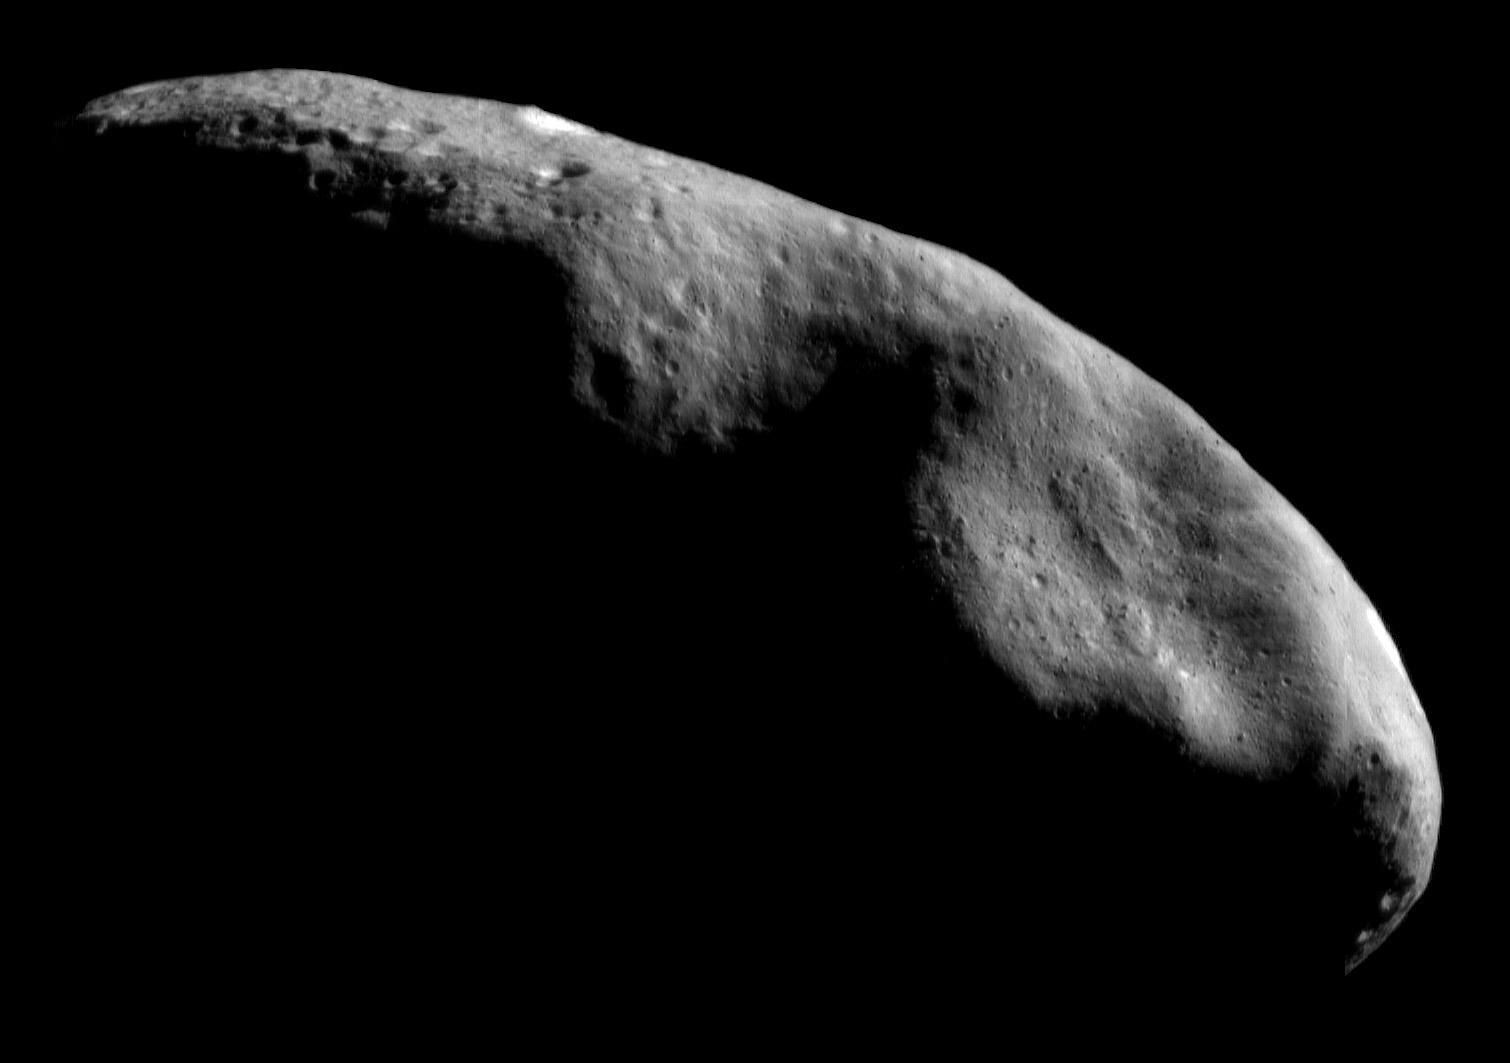
\includegraphics[height=0.5\textheight,width=0.5\textwidth,keepaspectratio]{figures/defense/near_mos_20001203_full.jpg}
    ~
    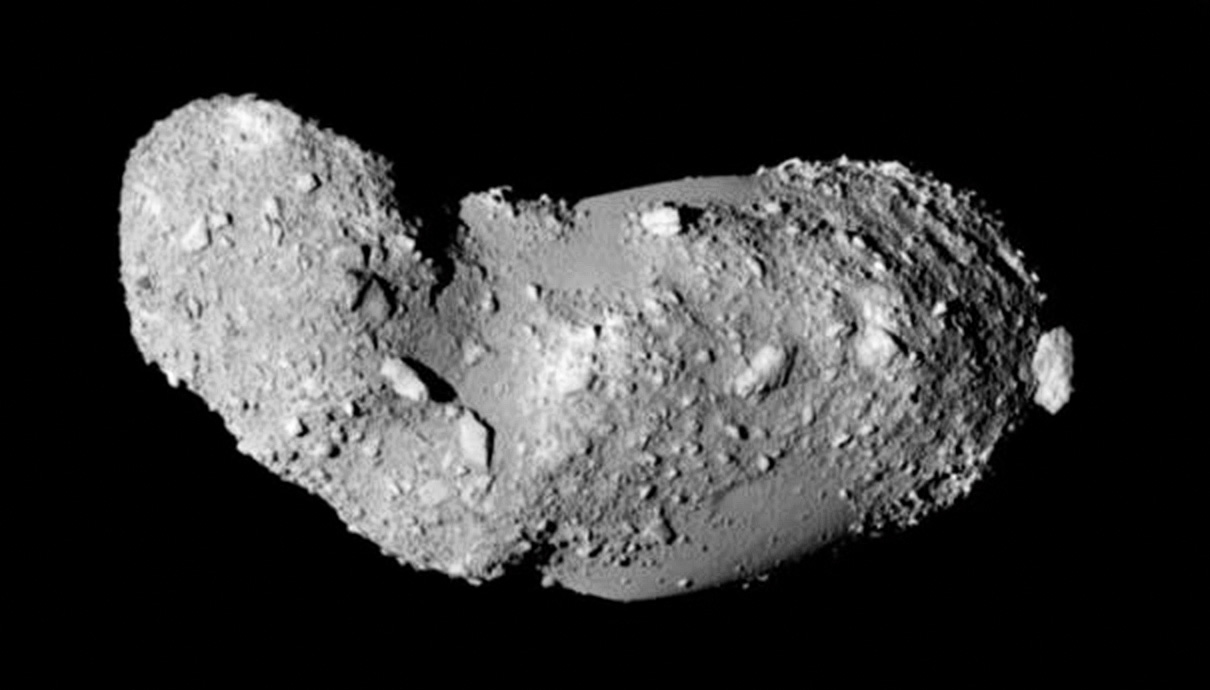
\includegraphics[height=0.5\textheight,width=0.5\textwidth,keepaspectratio]{figures/defense/Itokawa8_hayabusa_1210.jpg}
\end{center}
\end{frame}

\begin{frame}{Asteroid Mining}
    \begin{itemize}
      \item Useful materials can be extracted from asteroids to support:
      \begin{itemize}
          \item Propulsion, construction, life support, agriculture, and precious/strategic metals
      \end{itemize}
      \item Commercialization of near-Earth asteroids is feasible
    \end{itemize}

\pause

\begin{center}
\small
    \begin{tabular}{|l|r|r|}
        \hline 
        Element & Price (\SI{}{\$\per\kilo\gram}) & Sales (\SI{}{\$M\per yr}) \\
        \hline \hline 
        Phosphorous (P) & \num{0.08}  & \num{2167} \\
        Gallium (Ga) & \num{300.00}  & \num{1544} \\
        Germanium (Ge) & \num{745.00} & \num{6145} \\
        \hline \hline 
        Platinum (Pt) & \num{12394.00} & \num{1705} \\
        Gold (Au) & \num{12346.00} & \num{49} \\
        Osmium (Os) & \num{12860.00} & \num{307} \\
        \hline
    \end{tabular}
\end{center}

\end{frame}

\begin{frame}[t]{Problem statement}
    \begin{itemize}
        \item Ground based systems only provide a coarse shape estimate
        \item Spacecraft operations, e.g.\ landing, requires an accurate gravity model
        \item The gravity model accuracy is based on the accuracy of the shape
    \end{itemize}

    \begin{block}{}
        \begin{center}
            \begin{enumerate}
                \item Need an accurate shape before arrival
                \item Only in-situ measurements can provide the required detail
            \end{enumerate}
        \end{center}
    \end{block}
    
    This dissertation develops:
    \begin{enumerate}
        \item Correct dynamic model to predict motion of spacecraft,
        \item Control system to transfer around the small body,
        \item An efficient method to estimate and update the shape of the small body.
    \end{enumerate}
\end{frame}

\subsection[Electric Propulsion]{Electric Propulsion}  

\begin{frame} \label{slide:lowthrust_vehicles}%-----------------------------%
\frametitle{Low-thrust vehicles} % electric propulsion
\begin{itemize}
    \item Low-thrust orbital transfers offer increased mission oportunities
    \begin{itemize}
        \item Electric propulsion is increasing in capability
        \item Offers much higher specific impulse than chemical engines 
        \item Requires much longer operating periods for maneuvers 
        \item Enables long duration missions with frequent thrusting
    \end{itemize}
\end{itemize}

\begin{center}
    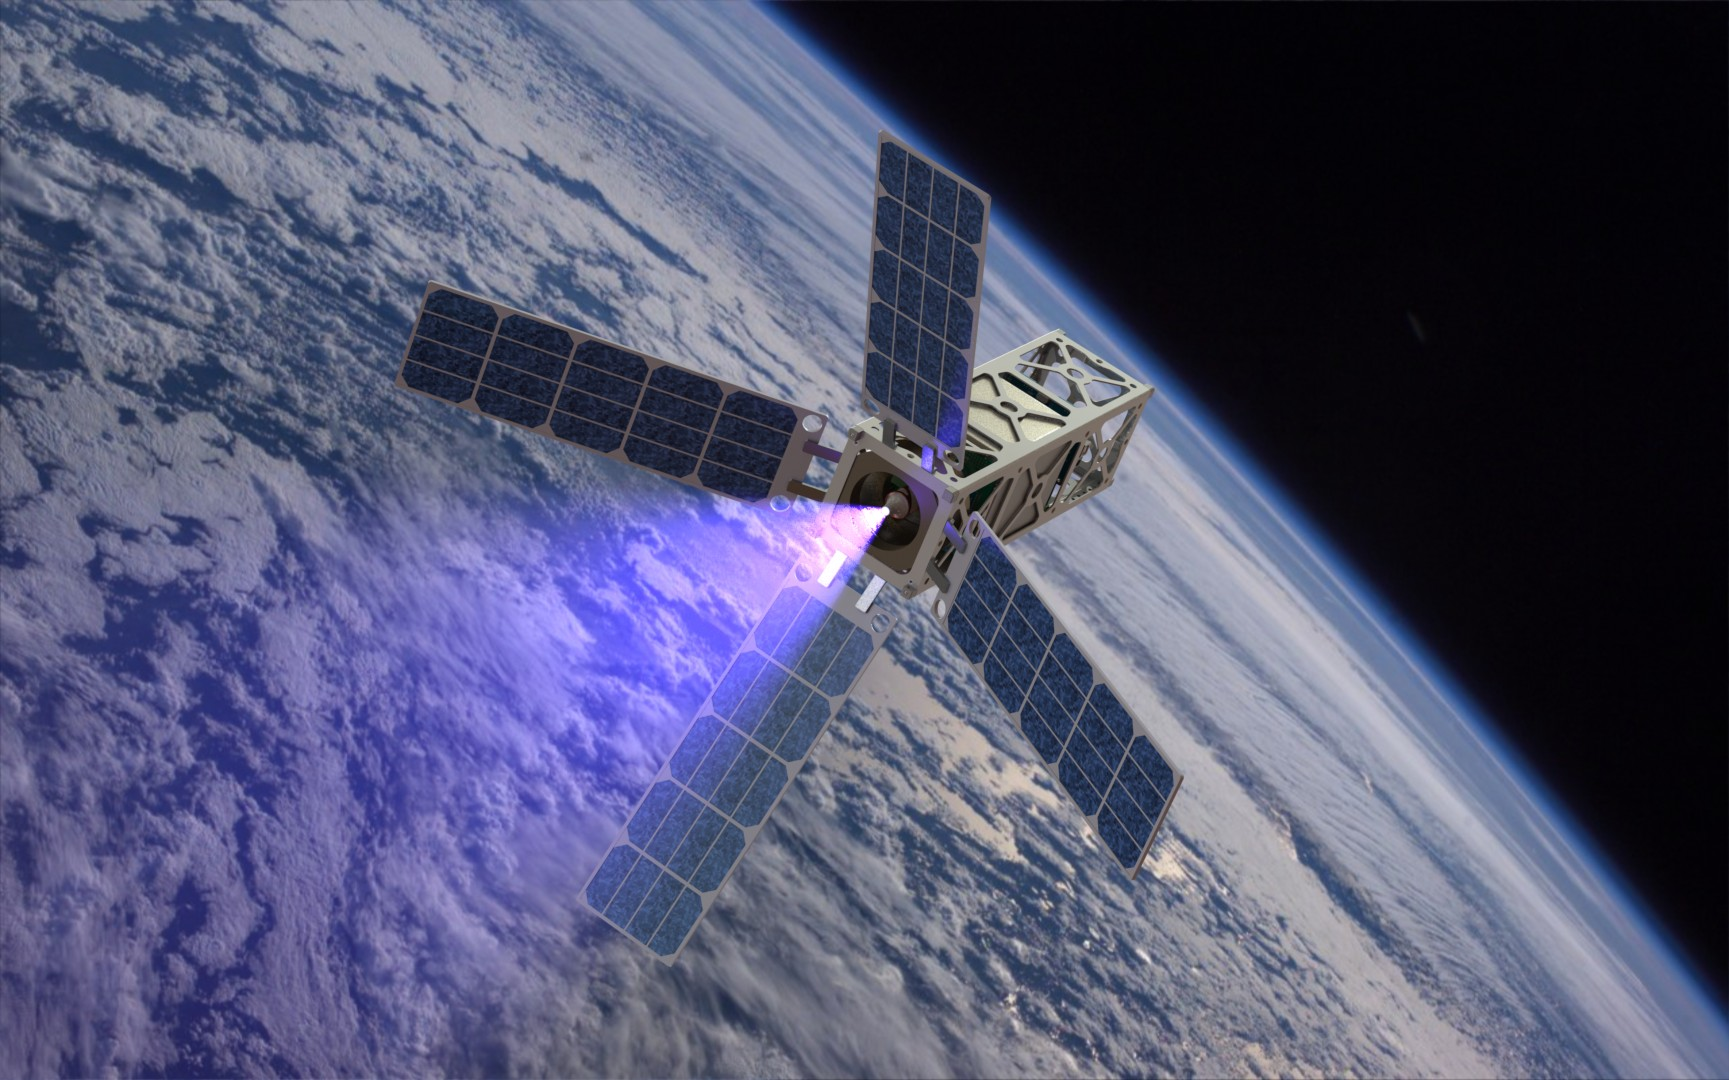
\includegraphics[height=0.4\textheight,width=0.5\textwidth,keepaspectratio]{figures/defense/patriot_plume.jpg}
    ~
    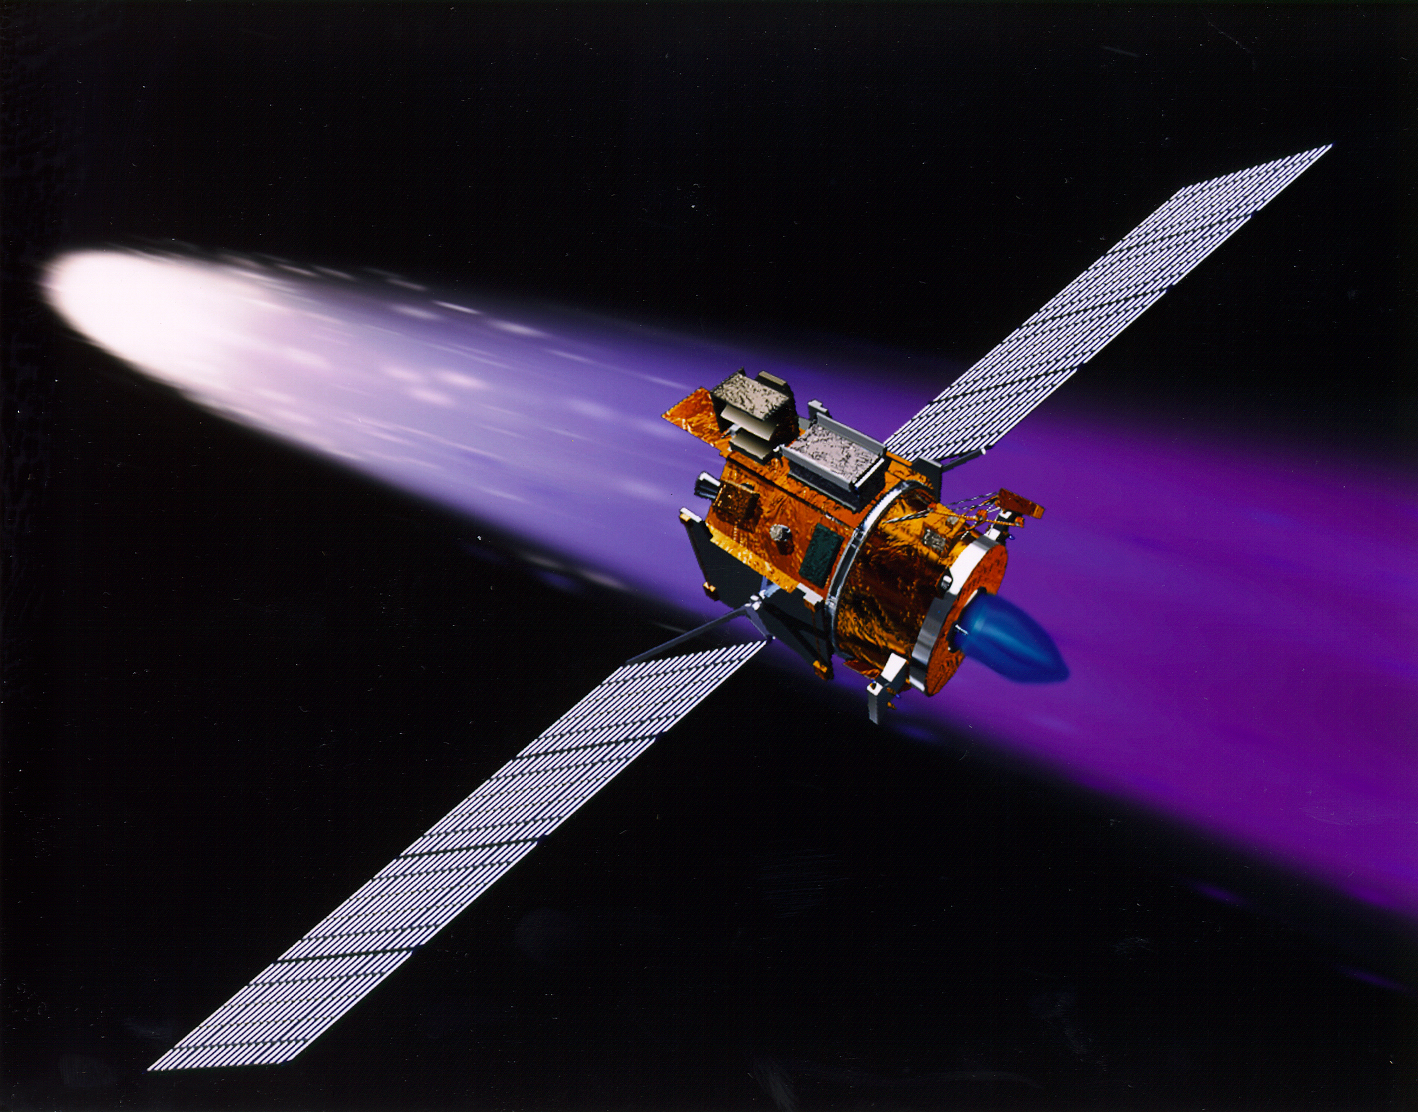
\includegraphics[height=0.4\textheight,width=0.5\textwidth,keepaspectratio]{figures/defense/deepspace1.jpg}
\end{center}
\hyperlink{slide:propulsion}{\beamergotobutton{Ideal Rockets}}
\end{frame}   %-----------------------------%

\subsection[Spacecraft Autonomy]{Spacecraft Autonomy}
% why study the coupled attitude/translational problem

\begin{frame}[t]{Spacecraft Autonomy} %-----------------------------%
\begin{itemize}
    \item Autonomous control of space vehicles is critical
    \begin{itemize}
        \item Avoid extensive planning and interaction by operators
        \item Ability to operate safely with system uncertainty 
        \item Independently navigate hazards and handle possible failures
    \end{itemize}
\end{itemize}
\visible<2>{
\begin{center}
    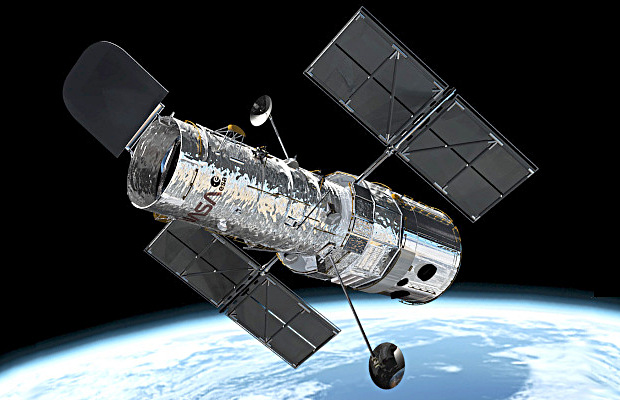
\includegraphics[width=0.5\textwidth,height=0.35\textheight,keepaspectratio]{figures/defense/hubble.jpg}\hfill
    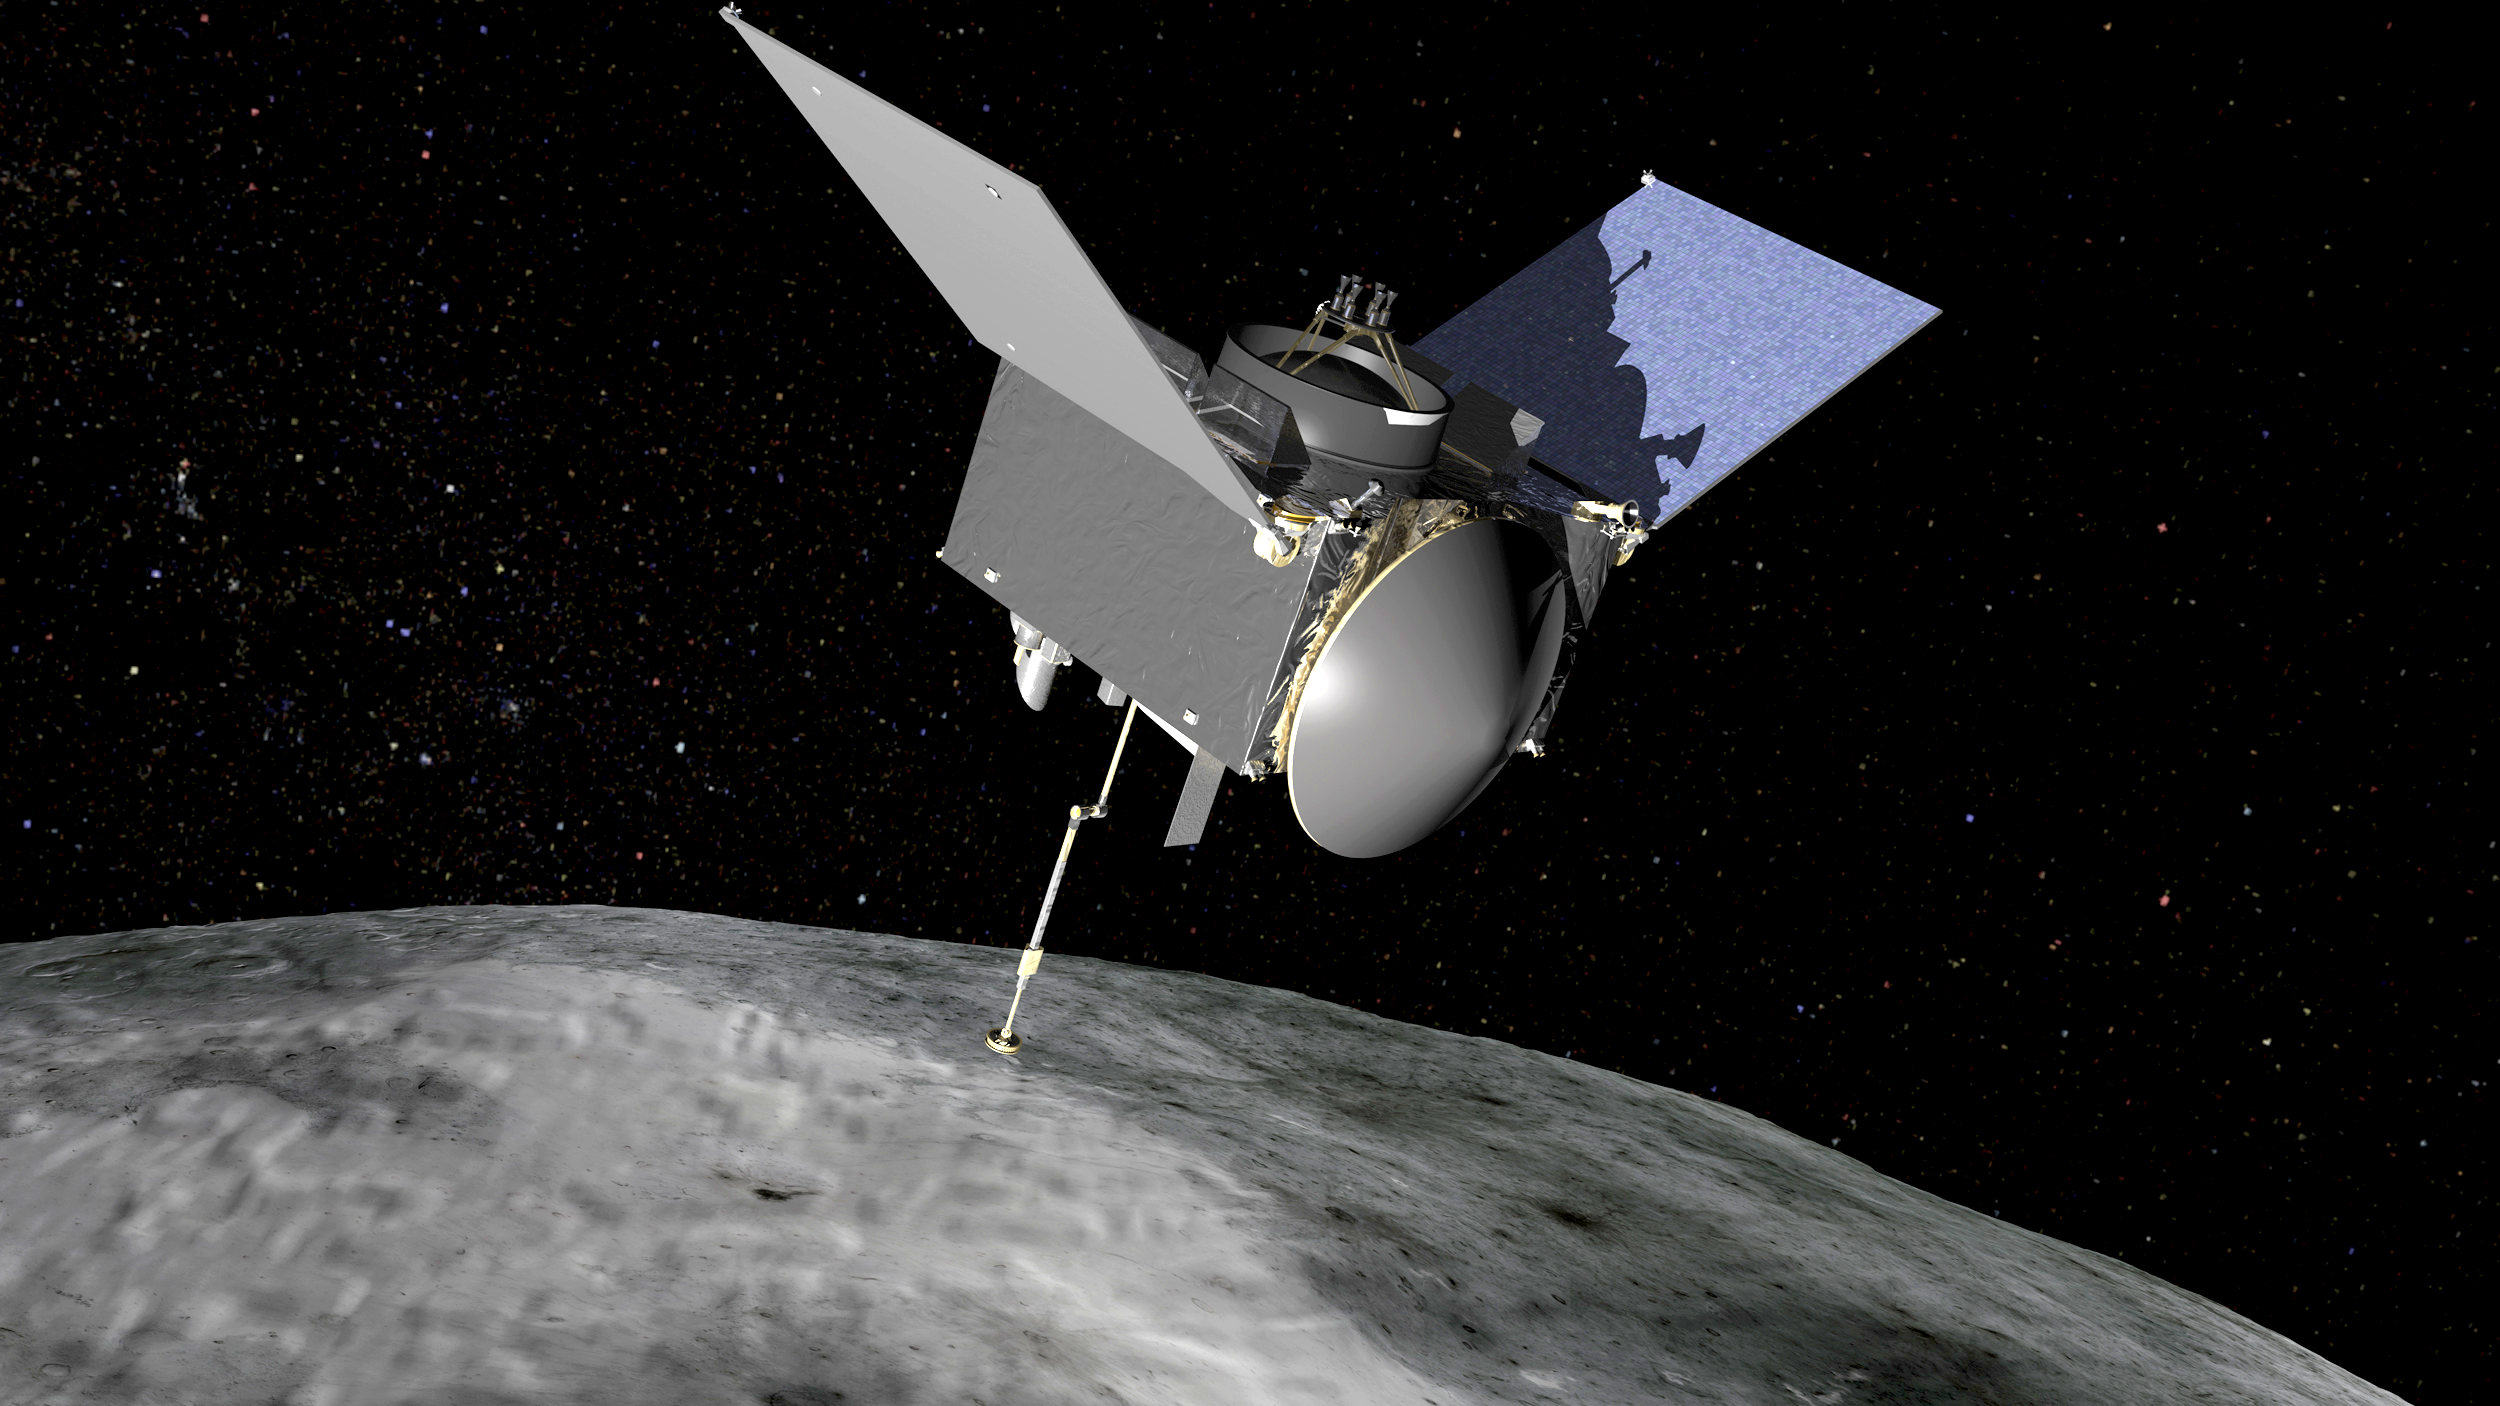
\includegraphics[width=0.5\textwidth,height=0.4\textheight,keepaspectratio]{figures/defense/osires_rex.png}
\end{center}
}
\note[itemize]{
    \item Autonomy is a key component to enable asteroid missions
}
\end{frame}   %-----------------------------%

\begin{frame}[t]{Why send spacecraft to asteroids?}
    \begin{itemize}
        \item<1-> Some properties only available at the asteroid:
            \begin{itemize}
                \item High fidelity gravitational model
                \item Surface samples or return missions
            \end{itemize}
        \item<2-> Gain experience for future missions
            \begin{itemize}
                \item Weak gravitational field allows for less costly manuevers
                \item Asteroid tours for future deep-space human missions
            \end{itemize}
        \item<3-> Avoiding future impacts
            \begin{itemize}
                \item Local spacecraft can aid in ground based tracking
                \item Mitigation: Gravity tractors, kinetic impactors, solar sails
            \end{itemize}
    \end{itemize}

\end{frame}


% !TEX Root = ../defense.tex

\section[Challenges]{Challenges in asteroid missions}
\subsection[Previous Approaches]{Drawbacks to previous approaches}

\begin{frame}{Challenges for Optimal Transfer Design} %-----------------------------%

\begin{itemize}
    \item Optimization in astrodynamics
        \begin{itemize}
            \item Orbital dynamics are nonlinear and chaotic
            \item Very sensitive to initial conditions
            \item Intuition required by designer to enable convergence
        \end{itemize}
    \pause
    \item Transfers using low-thrust propulsion
        \begin{itemize}
            \item Requires long periods of thrusting/coasting
            \item Small perturbations require accurate numerical integration
            \item Difficult to capture the long-term effects accurately
        \end{itemize}
    \pause
    \item Direct Optimal Control
        \begin{itemize}
            \item Reformulate problem as parameter optimization
            \item Allows for use of nonlinear programming methods
            \item High dimensional problem and computationally intensive
            \item Results in suboptimal solutions due to discretization
        \end{itemize}
\end{itemize}

\note[itemize]{
    \item Here we discuss some previous approaches to solve this asteroid mission problem and highlight their difficulties
    \item Optimization is very frequently used in astrodynamic applications
    \item Chaos - small changes of the initial conditions lead to large variations in the resulting trajectory
    \item Incorporating low thrust propulsion adds even more difficulty for optimization
}
\end{frame}   %-----------------------------%

\begin{frame}\label{slide:system_model_challenges}
\frametitle{Dynamic System Modelling}
\begin{itemize}
    \item Astrodynamics - motion of objects in space \hyperlink{astro}{\beamergotobutton{Intro to Astro}}
    \pause
    \item Attitude coupling is dependent on ratio \( \epsilon = \frac{l}{R} \)
        \begin{itemize}
            \item Typically ignored for Earth based missions 
            \item Force depends on attitude and oment depends on position
            \item Vastly different time scales
        \end{itemize}
\end{itemize}
\begin{align*}
    m \dot{v} &= m v \times \Omega + \sum F(b, R) \\
    J \dot{\Omega}  &= J \Omega \times \Omega +  \sum M(b, R) 
\end{align*}

\visible<2>{
\begin{center}
    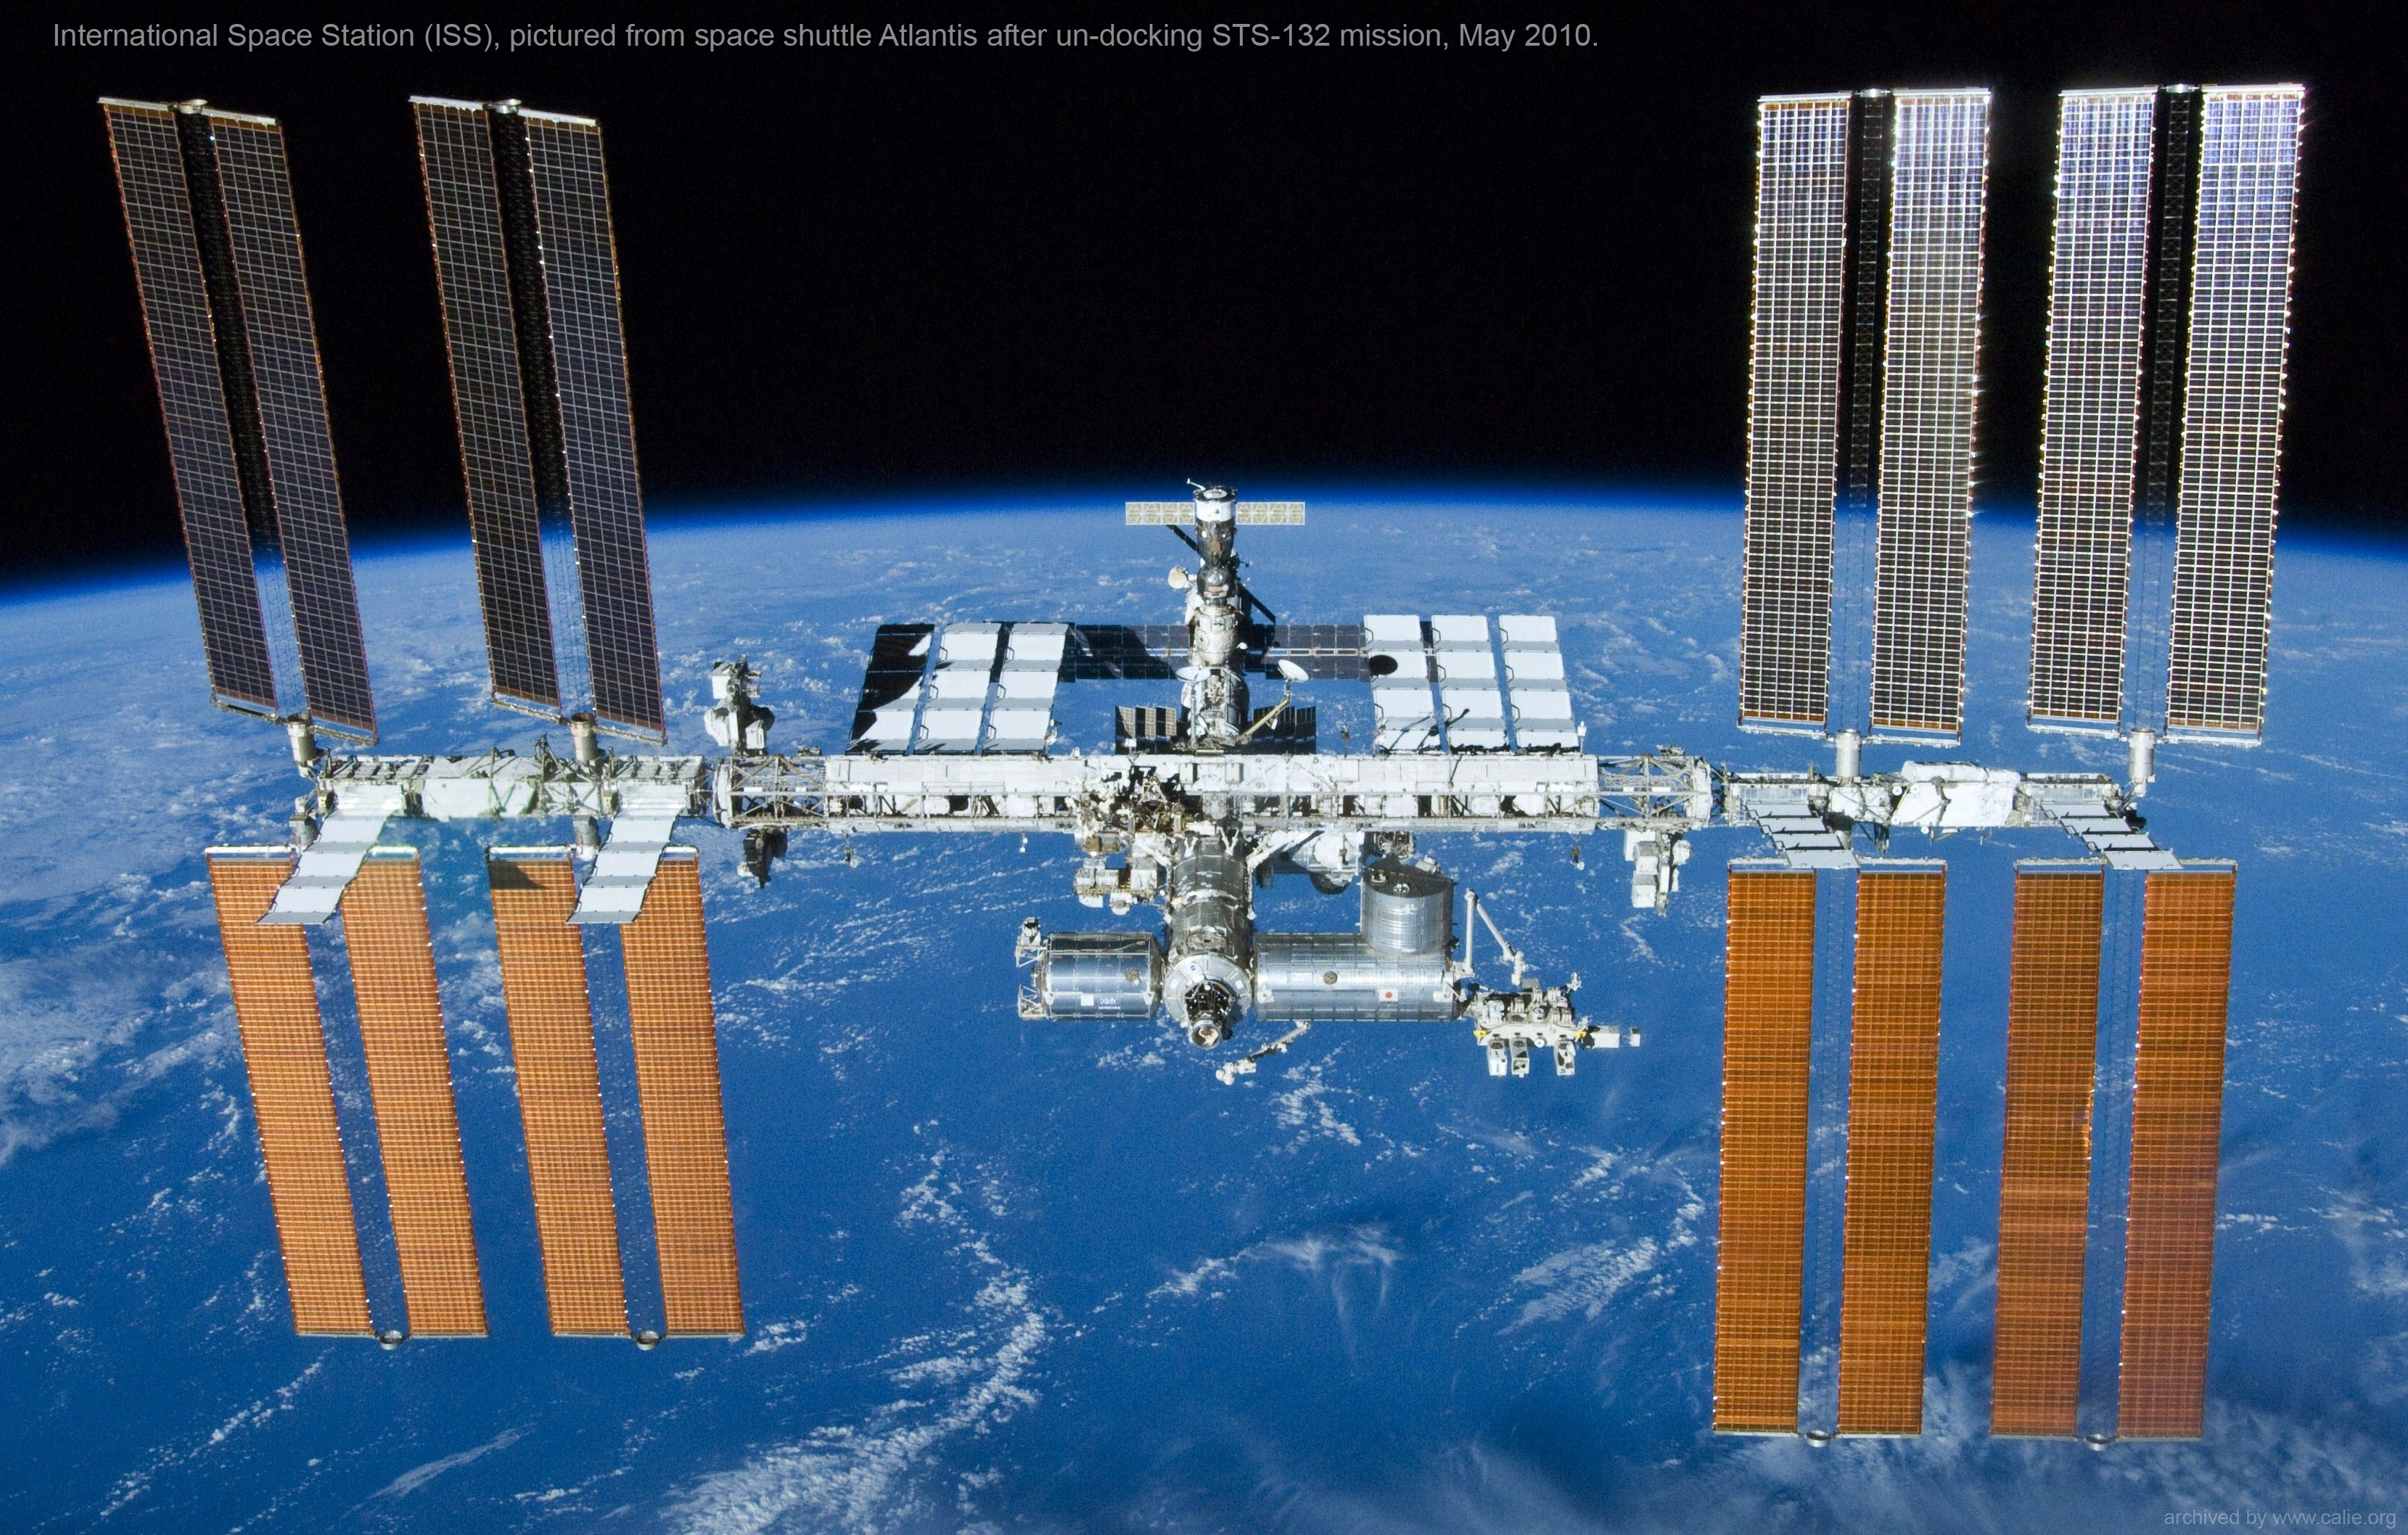
\includegraphics[width=0.5\textwidth,height=0.4\textheight,keepaspectratio]{figures/defense/ISS_STS-132.jpg}
    \quad
    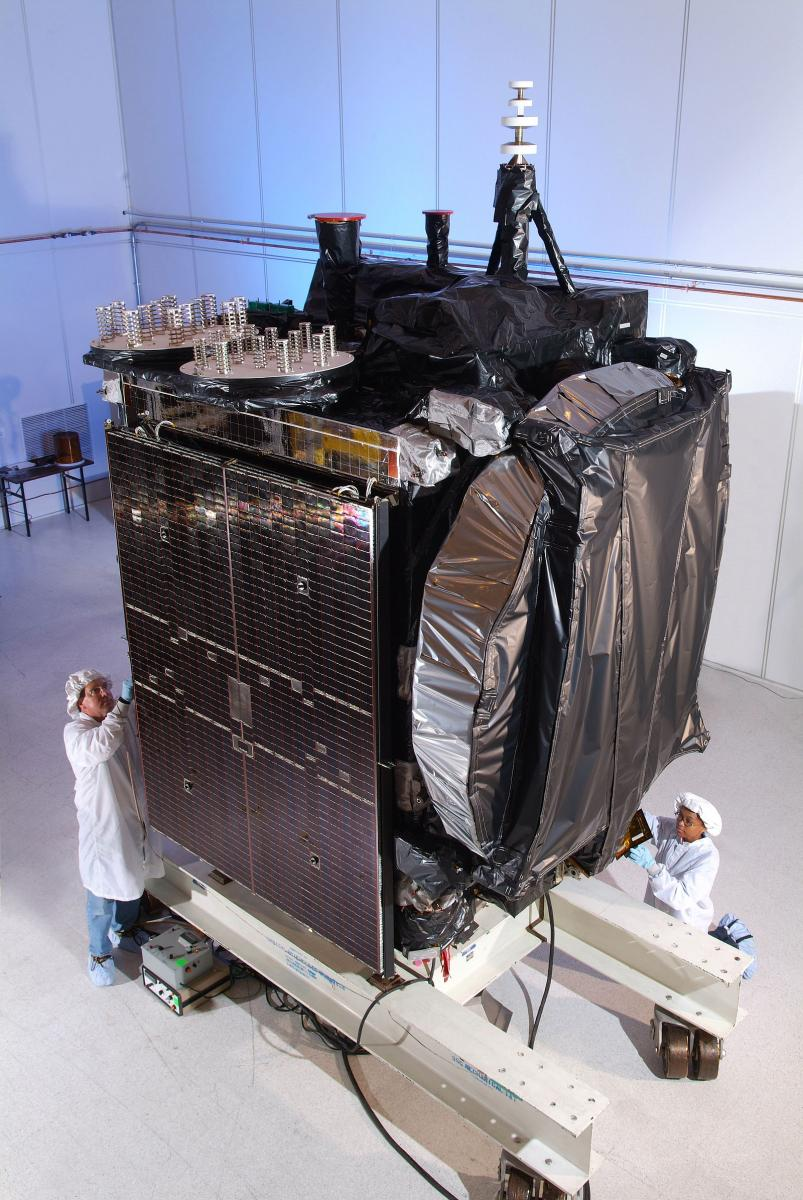
\includegraphics[width=0.5\textwidth,height=0.4\textheight,keepaspectratio]{figures/defense/Galaxy_15_photo.jpg}
\end{center}
}
\note[itemize]{
    \item Astrodynamics vs. Celestial mechanics - is the difference between the study of man-made or natural objects
    \item Typically consider all objects as point masses - disregard rotational dynamics
    \item In reality the translational and rotational dynamics are tightly coupled
    \item The coupled problem greatly increases the complexity
    \item Galaxy-15 is about a \SI{2}{\meter} cube, \SI{2500}{\kilo\gram}
    \item Located in GEO at \SI{133}{\degree} W
    \item Some attitude dependent forces - SRP, Drag, gravitational gradient
}

\end{frame}


\begin{frame}[t]{Planetary Landing} %-----------------------------------%
\begin{center}
    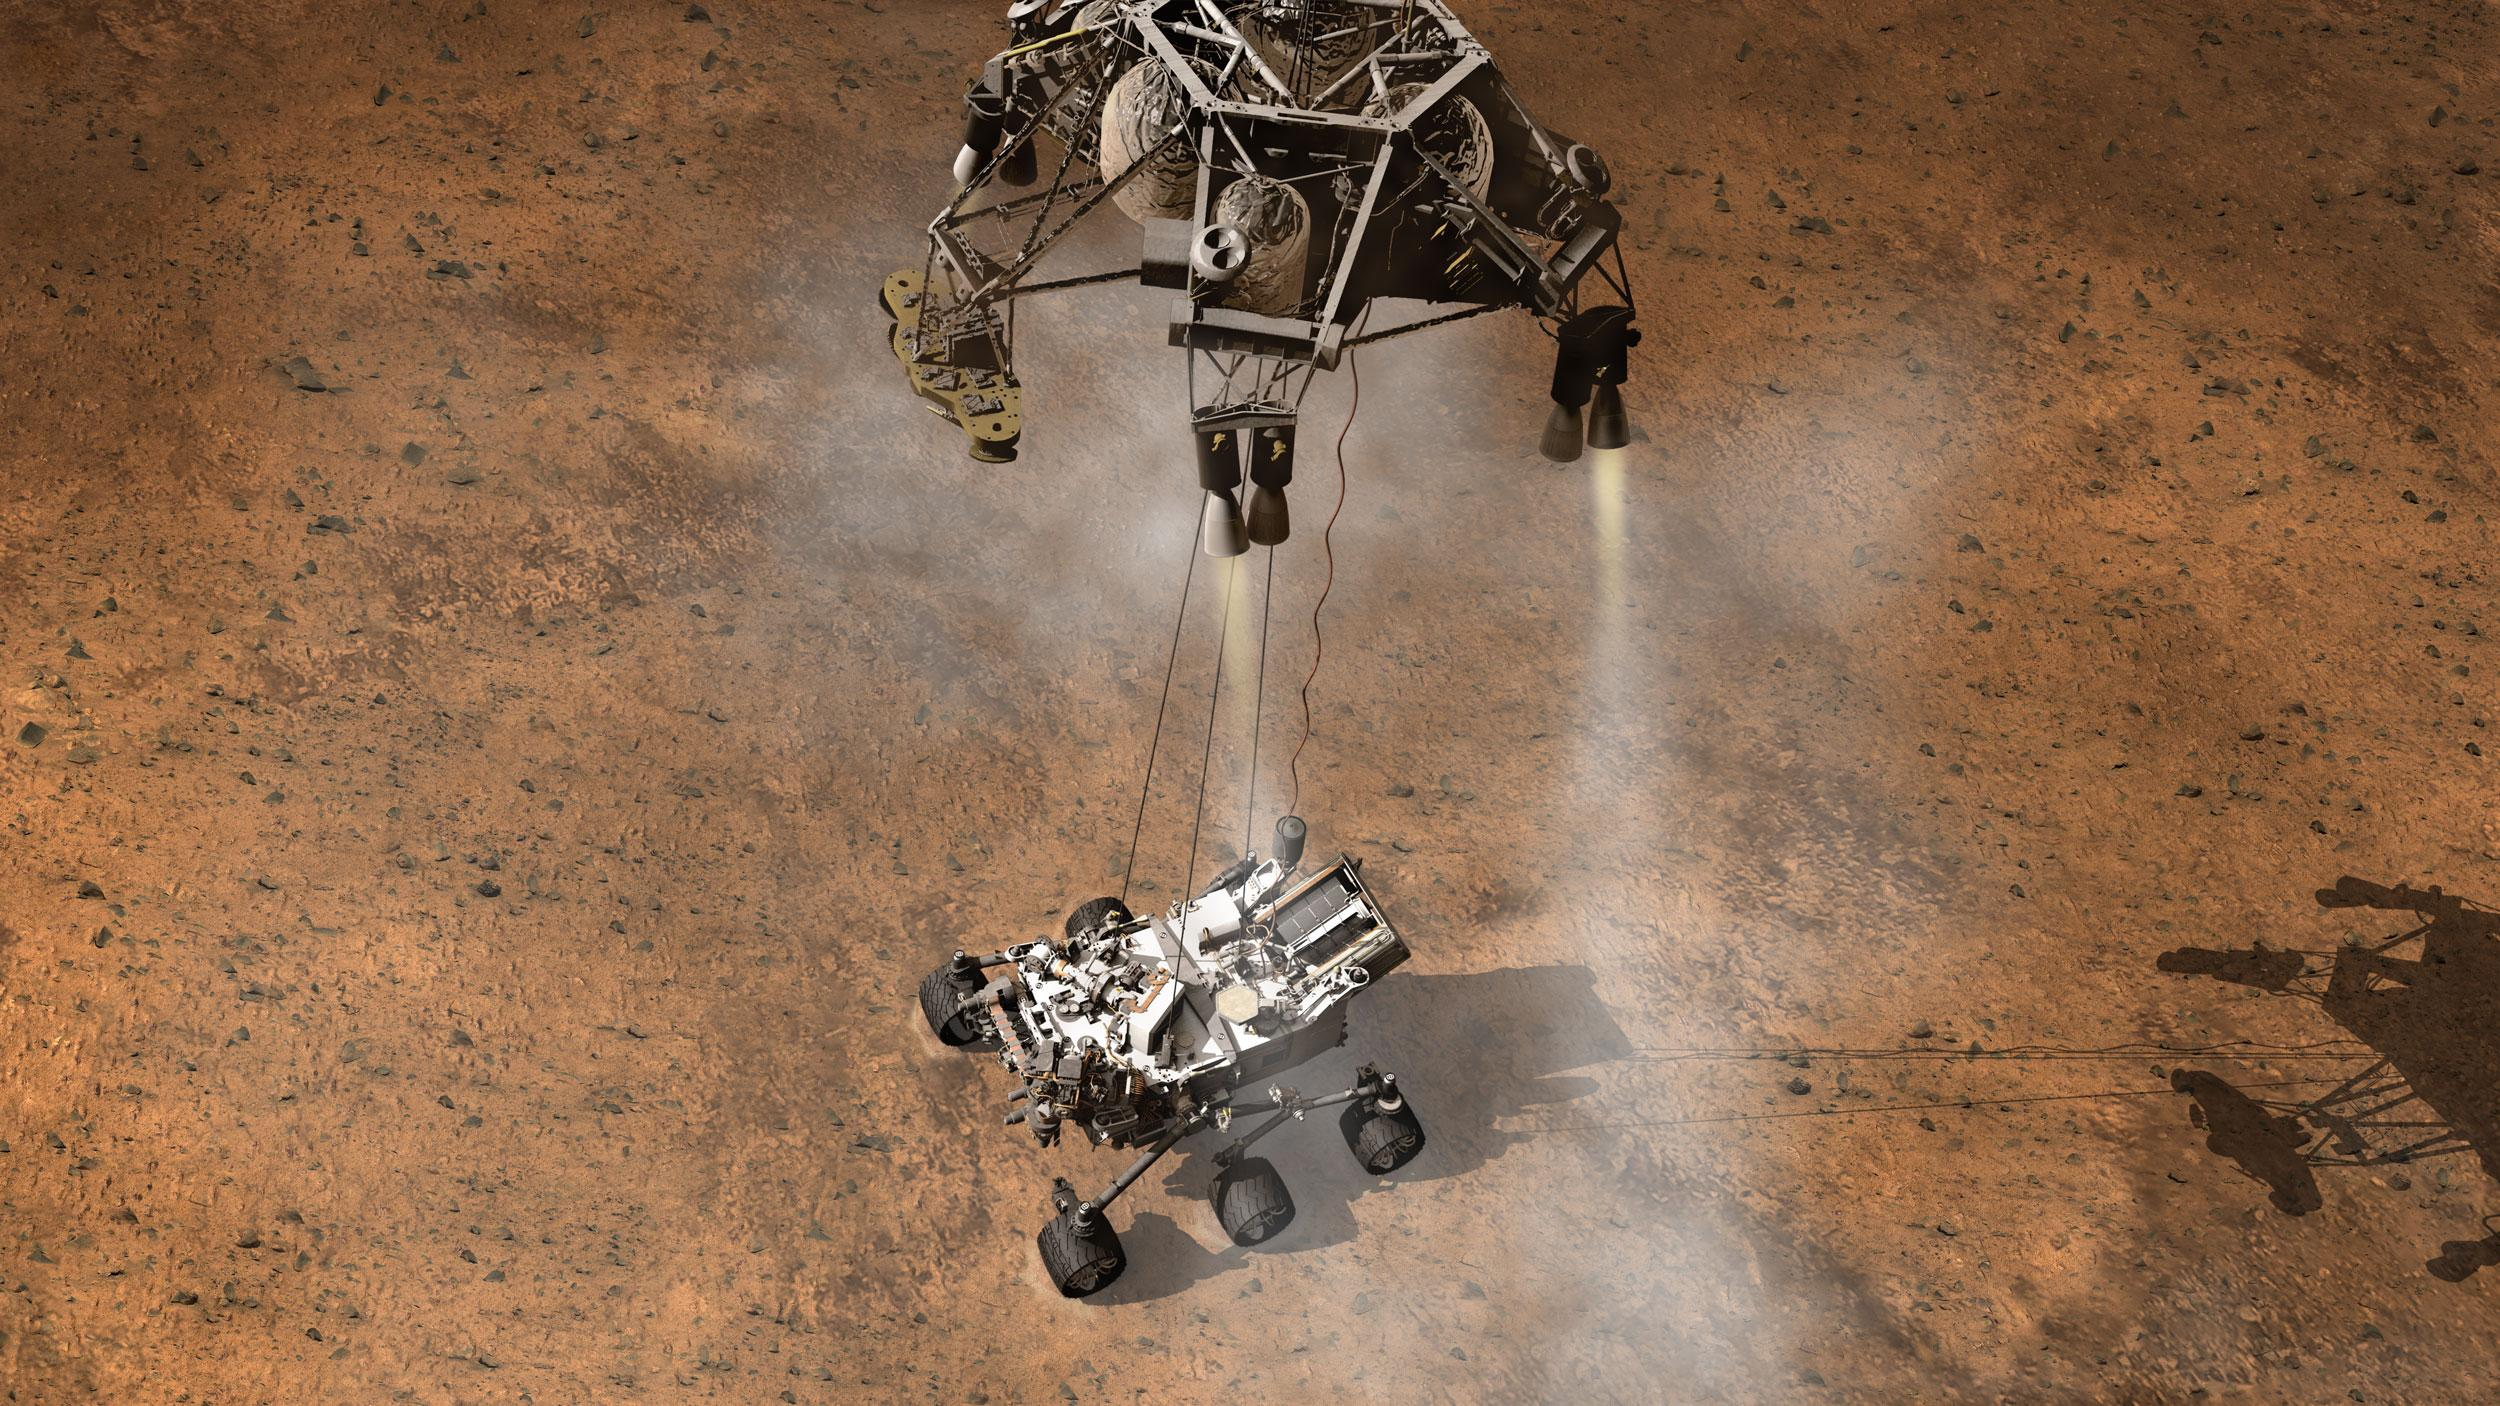
\includegraphics[width=0.5\textwidth,height=0.3\textheight,keepaspectratio]{figures/defense/curiosity.jpg} ~
    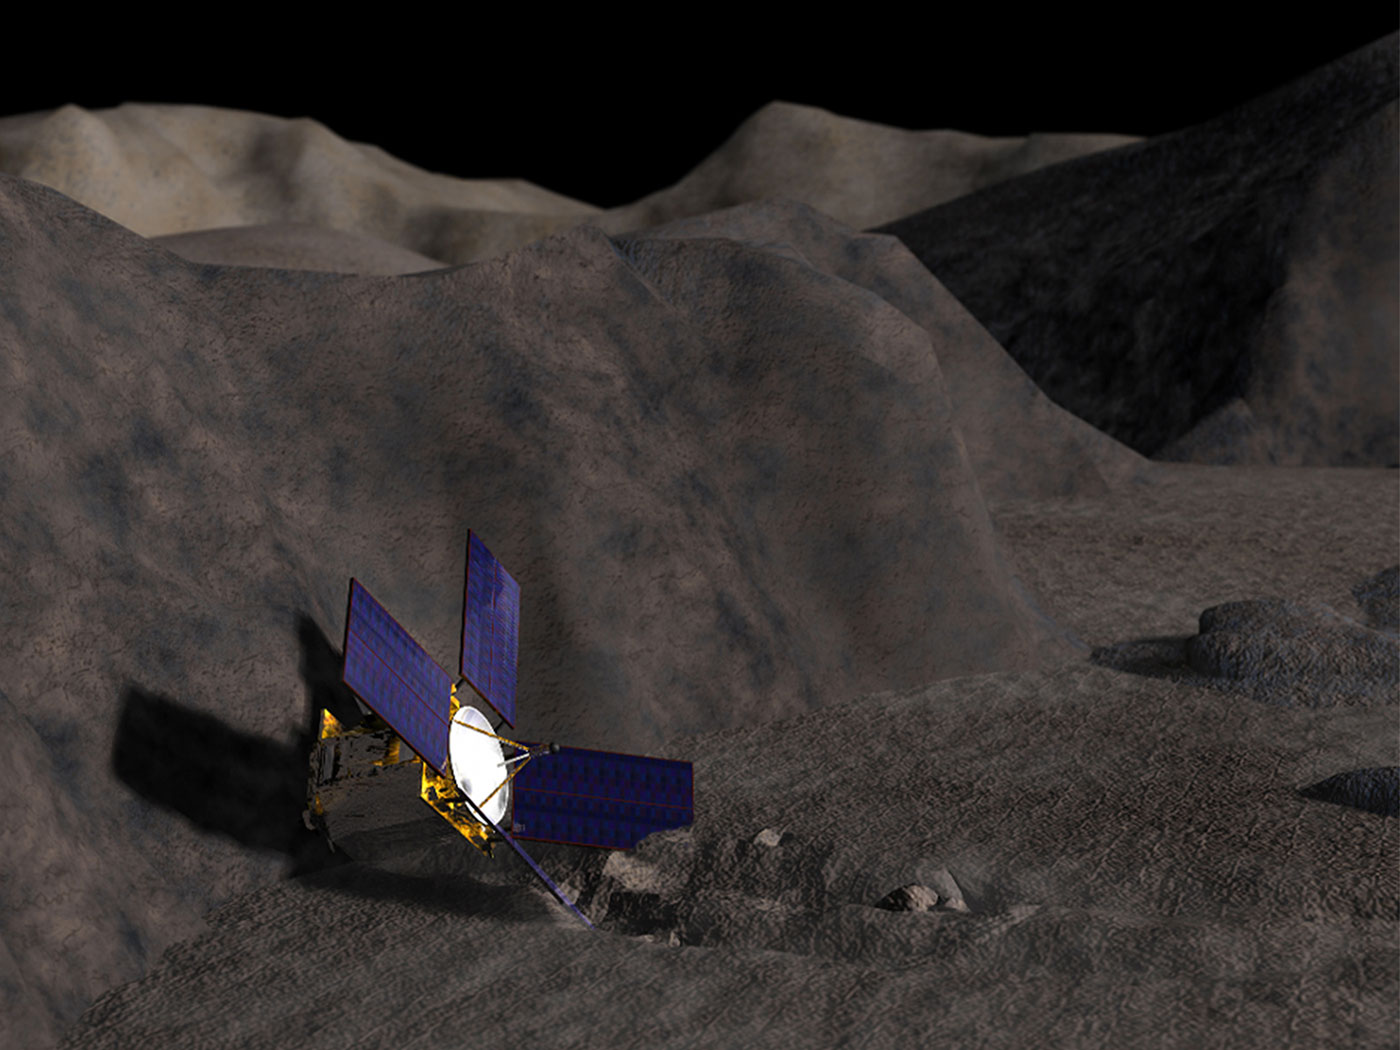
\includegraphics[width=0.5\textwidth,height=0.3\textheight,keepaspectratio]{figures/defense/430_new_landingnearstill.jpg}
\end{center}

\begin{itemize}
    \item Extensive history of manned/unmanned planetary landings
    \pause
    \item Previous approaches highly resource dependent
    \begin{itemize}
        \item Typically rely on offline optimization
        \item Extensive human planning and analysis
    \end{itemize}
\end{itemize}
\pause
\begin{block}{Drawback of Open Loop Control}
    \begin{itemize}
        \item Not robust to errors in dynamic model
        \item Unable to handle failures
        \item Unable to react to varying obstacle or constraints
    \end{itemize}
\end{block}

\note[itemize]{
    \item We show the now famous Curiosity and it's skycrane as well as the relatively less impressive NEAR, which isn't even designed for landing but did anyways
}
\end{frame} %-------------------------------------%



% mathematical background
% !TEX root = ../../defense.tex

\section{Dynamic Model}

\begin{frame}{Reference Frames}

    \begin{columns}
        \begin{column}{0.5\textwidth}
            \begin{enumerate}
                \item \( \vc{e}_i \in \R^3 \) : inertial reference frame fixed in space
                \item \( \vc{f}_i \in \R^3 \) : small body fixed frame aligned with principle axes of the body
                \item \( \vc{b}_i \in \R^3 \) : spacecraft fixed frame with \( b_1 \) aligned with the symmetry axis
            \end{enumerate}
            
            \begin{block}{}
                Spacecraft state is defined on the Special Euclidean group

                \[ \parenth{R, \vc{x}} \in \SE \]
            \end{block}
        \end{column}
        \begin{column}{0.5\textwidth}
            \begin{scaletikzpicturetowidth}{2\columnwidth}
                \resizebox{\columnwidth}{!}{%
                %set the plot display orientation
%synatax: \tdplotsetdisplay{\theta_d}{\phi_d}
\tikzsetnextfilename{ref_frames}
\tdplotsetmaincoords{60}{110}
%start tikz picture, and use the tdplot_main_coords style to implement the display 
%coordinate transformation provided by 3dplot
\begin{tikzpicture}[scale=5,tdplot_main_coords]
%define polar coordinates for some vector
\pgfmathsetmacro{\rvec}{.8}
\pgfmathsetmacro{\thetavec}{30}
\pgfmathsetmacro{\phivec}{60}
\pgfmathsetmacro{\Px}{0.2}
\pgfmathsetmacro{\Py}{0.346}
\pgfmathsetmacro{\Pz}{0.693}
\pgfmathsetmacro{\b}{0.5}
\pgfmathsetmacro{\d}{0.3}

%set up some coordinates 
%-----------------------
\coordinate (O) at (0,0,0);
\coordinate (Ptikz) at (\Px, \Py, \Pz);
%determine a coordinate (P) using (r,\theta,\phi) coordinates.  This command
%also determines (Pxy), (Pxz), and (Pyz): the xy-, xz-, and yz-projections
%of the point (P).
%syntax: \tdplotsetcoord{Coordinate name without parentheses}{r}{\theta}{\phi}
% \tdplotsetcoord{P}{\rvec}{\thetavec}{\phivec}
%draw figure contents
%--------------------

%draw the main coordinate system axes
\draw[thick,-Latex] (0,0,0) -- (1,0,0) node[anchor=north east]{$e_1$};
\draw[thick,-Latex] (0,0,0) -- (0,1,0) node[anchor=north west]{$e_2$};
\draw[thick,-Latex] (0,0,0) -- (0,0,1) node[anchor=south]{$e_3 = f_3$};

%draw a vector from origin to point (P) 
\draw[-stealth,color=red, -Latex] (O) -- node [below right] {$ r $} ($(\Px, \Py, \Pz) $);

%draw the angle \phi, and label it
%syntax: \tdplotdrawarc[coordinate frame, draw options]{center point}{r}{angle}{label options}{label}
\tdplotdrawarc{(O)}{0.2}{0}{\phivec}{anchor=north}{$\Omega_A t$}


%set the rotated coordinate system so the x'-y' plane lies within the
%"theta plane" of the main coordinate system
%syntax: \tdplotsetthetaplanecoords{\phi}
\tdplotsetthetaplanecoords{\phivec}

% draw the asteroid frame
% \draw[thick,->,tdplot_rotated_coords] (0,0,0) -- (1,0,0) node[anchor=north east]{$f_3$};
\draw[thick,-Latex,tdplot_rotated_coords] (0,0,0) -- (0,1,0) node[anchor=north west]{$f_1$};
% \draw[thick,->,tdplot_rotated_coords] (0,0,0) -- (0,0,1) node[anchor=north west]{$f_2$};

%draw some dashed arcs, demonstrating direct arc drawing
\draw[dashed,tdplot_rotated_coords] (\rvec,0,0) arc (0:90:\rvec);
\draw[dashed] (\rvec,0,0) arc (0:90:\rvec);

%set the rotated coordinate definition within display using a translation
%coordinate and Euler angles in the "z(\alpha)y(\beta)z(\gamma)" euler rotation convention
%syntax: \tdplotsetrotatedcoords{\alpha}{\beta}{\gamma}
\tdplotsetrotatedcoords{\phivec}{\thetavec}{0}

%translate the rotated coordinate system
%syntax: \tdplotsetrotatedcoordsorigin{point}
\tdplotsetrotatedcoordsorigin{(Ptikz)}

%use the tdplot_rotated_coords style to work in the rotated, translated coordinate frame
\draw[thick,tdplot_rotated_coords,-Latex] (0,0,0) -- (\b,0,0) node[anchor=north west]{$b_1$};
\draw[thick,tdplot_rotated_coords,-Latex] (0,0,0) -- (0,\b,0) node[anchor=west]{$b_2$};
\draw[thick,tdplot_rotated_coords,-Latex] (0,0,0) -- (0,0,\b) node[anchor=south]{$b_3$};

% transform the first dumbbell
% rot to main
\tdplottransformrotmain{\d}{0}{0};
\tdplottransformmainscreen{\tdplotresx}{\tdplotresy}{\tdplotresz};
\pgfmathsetmacro{\DMonescreenx}{\tdplotresx};
\pgfmathsetmacro{\DMonescreeny}{\tdplotresy};

\tdplottransformrotmain{-\d}{0}{0};
\tdplottransformmainscreen{\tdplotresx}{\tdplotresy}{\tdplotresz};
\pgfmathsetmacro{\DMtwoscreenx}{\tdplotresx};
\pgfmathsetmacro{\DMtwoscreeny}{\tdplotresy};

% transform P to screen coordinates and then add
\tdplottransformmainscreen{\Px}{\Py}{\Pz};
\pgfmathsetmacro{\Pscreenx}{\tdplotresx};
\pgfmathsetmacro{\Pscreeny}{\tdplotresy};

\draw[ultra thick, color=blue, tdplot_rotated_coords] (-\d, 0, 0) -- (\d, 0, 0);

\shade[ball color=red, tdplot_screen_coords, opacity=0.3] (\Pscreenx, \Pscreeny) circle (0.03);
\shade[ball color=blue,tdplot_screen_coords] ($(\Pscreenx, \Pscreeny) + (\DMonescreenx, \DMonescreeny) + (0, 0.015)$) circle (0.03);
\shade[ball color=blue,tdplot_screen_coords] ($(\Pscreenx, \Pscreeny) + (\DMtwoscreenx, \DMtwoscreeny) + (0, -0.015)$ ) circle (0.03);

\end{tikzpicture}


            }
            \end{scaletikzpicturetowidth}
        \end{column}
    \end{columns}
\end{frame}

\begin{frame}{Spacecraft Model}
    \begin{itemize}
        \item Spacecraft modeled as a rigid dumbbell
        \item Two masses \( m_1, m_2 \in \R^1 \) connected by a rigid massless link \( l \in \R^1\)
        \item Effectively captures the mass distribution of a spacecraft
    \end{itemize}

    \resizebox{\textwidth}{!}{%
        %% helper macros

\newcommand\pgfmathsinandcos[3]{%
  \pgfmathsetmacro#1{sin(#3)}%
  \pgfmathsetmacro#2{cos(#3)}%
}
\newcommand\LongitudePlane[3][current plane]{%
  \pgfmathsinandcos\sinEl\cosEl{#2} % elevation
  \pgfmathsinandcos\sint\cost{#3} % azimuth
  \tikzset{#1/.style={cm={\cost,\sint*\sinEl,0,\cosEl,(0,0)}}}
}
\newcommand\LatitudePlane[3][current plane]{%
  \pgfmathsinandcos\sinEl\cosEl{#2} % elevation
  \pgfmathsinandcos\sint\cost{#3} % latitude
  \pgfmathsetmacro\yshift{\cosEl*\sint}
  \tikzset{#1/.style={cm={\cost,0,0,\cost*\sinEl,(0,\yshift)}}} %
}

\newcommand\DrawLongitudeCircle[4][1]{
\LongitudePlane{\angEl}{#2}
\tikzset{current plane/.prefix style={scale=#1}}
% angle of "visibility"
\pgfmathsetmacro\angVis{
atan(sin(#2)*cos(\angEl)/sin(\angEl))} %
\draw[shift={(#3, #4)}][current plane]
(\angVis:1) arc (\angVis:\angVis+180:1);
\draw[shift={(#3, #4)}][current plane,dashed]
(\angVis-180:1)arc(\angVis-180:\angVis:1);
}
\newcommand\DrawLatitudeCircle[4][1]{
\LatitudePlane{\angEl}{#2}
\tikzset{current plane/.prefix style={scale=#1}}
\pgfmathsetmacro\sinVis{
sin(#2)/cos(#2)*sin(\angEl)/cos(\angEl)}
% angle of "visibility"
\pgfmathsetmacro\angVis{
asin(min(1,max(\sinVis,-1)))}
\draw[shift={(#3, #4)}][current plane]
(\angVis:1) arc (\angVis:-\angVis-180:1);
\draw[shift={(#3, #4)}][current plane,dashed]
(180-\angVis:1)arc(180-\angVis:\angVis:1);
}

%% document-wide tikz options and styles

\tikzset{%
  >=latex, % option for nice arrows
  inner sep=0pt,%
  outer sep=2pt,%
  mark coordinate/.style={inner sep=0pt,outer sep=0pt,minimum size=3pt,
    fill=black,circle}%
}

\tikzsetnextfilename{dumbbell}
\begin{tikzpicture} % "THE GLOBE" showcase

\def\R{2} % sphere radius
\def\angEl{35} % elevation angle
\def\angAz{-105} % azimuth angle
\def\length{4} % distance from COM to M_1
\def\opacity{0.2}

% centers of the masses
\coordinate (m1) at (\length, 0);
\coordinate (m2) at (-\length, 0);

\draw [ thick, dashed, -Latex] (m2) -- ($ (m1) + (3, 0) $) node [below right] {$b_1$};
\draw [thick, dashed, -Latex] (0, 0) -- (0, \R) node [above right] {$b_2$};
% TODO Make a macro to draw a sphere at a sphefic point
\filldraw[ball color=blue, opacity=\opacity] (m1) circle (\R);
\foreach \t in {-45, 0, 45} { \DrawLatitudeCircle[\R]{\t}{\length}{0} }
\foreach \t in {-30, -60,...,-150} { \DrawLongitudeCircle[\R]{\t}{\length}{0} }

\filldraw[ball color=blue, opacity=\opacity] (m2) circle (\R);
\foreach \t in {-60,-30,...,60} { \DrawLatitudeCircle[\R]{\t}{-\length}{0} }
\foreach \t in {-5,-35,...,-175} { \DrawLongitudeCircle[\R]{\t}{-\length}{0} }

% draw from origin to center of m1
\draw[thick,-Latex] node [below right] {$\zeta$} (0, 0) --  (m1);
\draw[thick,-Latex] (m1) -- ++(30:\R) node [above right] {$\eta$};
\end{tikzpicture}


    }
\end{frame}

\begin{frame}{Equations of Motion}
    Hamilton's principle used to derive equations of motion in four forms:
    \begin{enumerate}
        \item Inertial vs. Relative 
        \item Lagrangian vs. Hamiltonian
    \end{enumerate}
    True motion of the system is a stationary point of the action integral
    \begin{align*}
        \mathcal{G} &= \int_{t_0}^{t_f} T(\dot q) - V(q) dt\\
        \delta \mathcal{G} &= \int_{t_0}^{t_f} \delta T - \delta V dt = 0
    \end{align*}
\end{frame}

\begin{frame}{Inertial EOMs in Lagrangian Form}
    The kinetic and potential energy of the dumbbell in the inertial frame
    \begin{align*}
        T\parenth{\dot{\ipos}, \iangvel} &= \frac{1}{2} m \norm{\dot{\vc{x}}}^2 + \frac{1}{2} \tr{\vh{\Omega} J_d \vh{\Omega}^T} , \\
        V( \ipos, R ) &=  - m_1 U \parenth{R_A^T \parenth{\vc{x} + R \vc{\rho}_1}} - m_2 U \parenth{R_A^T \parenth{\vc{x} + R \vc{\rho}_2}}. 
    \end{align*}
    The stationary point of the action integral gives:
    \begin{align*}
        \dot{\ipos} &= \ivel, \\
        \parenth{m_1 + m_2} \dot{\ivel} &= - \sum_{i=0}^2 m_i \aatt \deriv{U}{\apos_i} + u_f, \\
        \dot{\iatt} &= \iatt \iangvel, \\
        J \dot{\iangvel} + \hat{\iangvel} J \iangvel &= \sum_{i=0}^2 m_i \hat{\spos}_i \iatt^T \aatt \deriv{U}{\apos_i} + u_m. 
    \end{align*}
\end{frame}

\begin{frame}{Relative Equations of Motion}

\begin{itemize}
    \item Gravitational potential is a function of relative position
    \item Can derive EOMs in the rotating small body fixed frame
    \item Kinematics defined relative to the small body
\end{itemize}

\begin{align*}
    \dot{x}_r &= \rvel - \hat{\Omega}_A \rpos, \\
    \parenth{m_1 + m_2} \dot{v}_r  &= -\parenth{m_1 + m_2} \hat{\Omega}_A \rvel + m_1 \deriv{U}{z_1} + m_2 \deriv{U}{z_2}, \\
    \dot{R}_r &= \hat{\Omega}_r \ratt  - \hat{\Omega}_A \ratt , \\
    \dot{\parenth{\Jr  \rangvel}} + \hat{\Omega}_A \parenth{\Jr  \rangvel} &= m_1 \parenth{\ratt  \rho_1}^\wedge \deriv{U}{z_1} + m_2 \parenth{\ratt  \rho_2}^\wedge \deriv{U}{z_2}.
\end{align*}
\end{frame}

% system model

% low thrust propulsion/nonlinear control
% !TEX root = ../../defense.tex

\section{Low Thrust Transfer}

\begin{frame} \label{slide:lowthrust_vehicles}%-----------------------------%
\frametitle{Low thrust vehicles} % electric propulsion
\begin{itemize}
    \item Low thrust orbital transfers offer increased mission oportunities
    \begin{itemize}
        \item Electric propulsion is increasing in capability
        \item Offers much higher specific impulse than chemical engines 
        \item Requires much longer operating periods for maneuvers 
        \item Enables long duration missions with frequent thrusting
    \end{itemize}
\end{itemize}

\begin{center}
    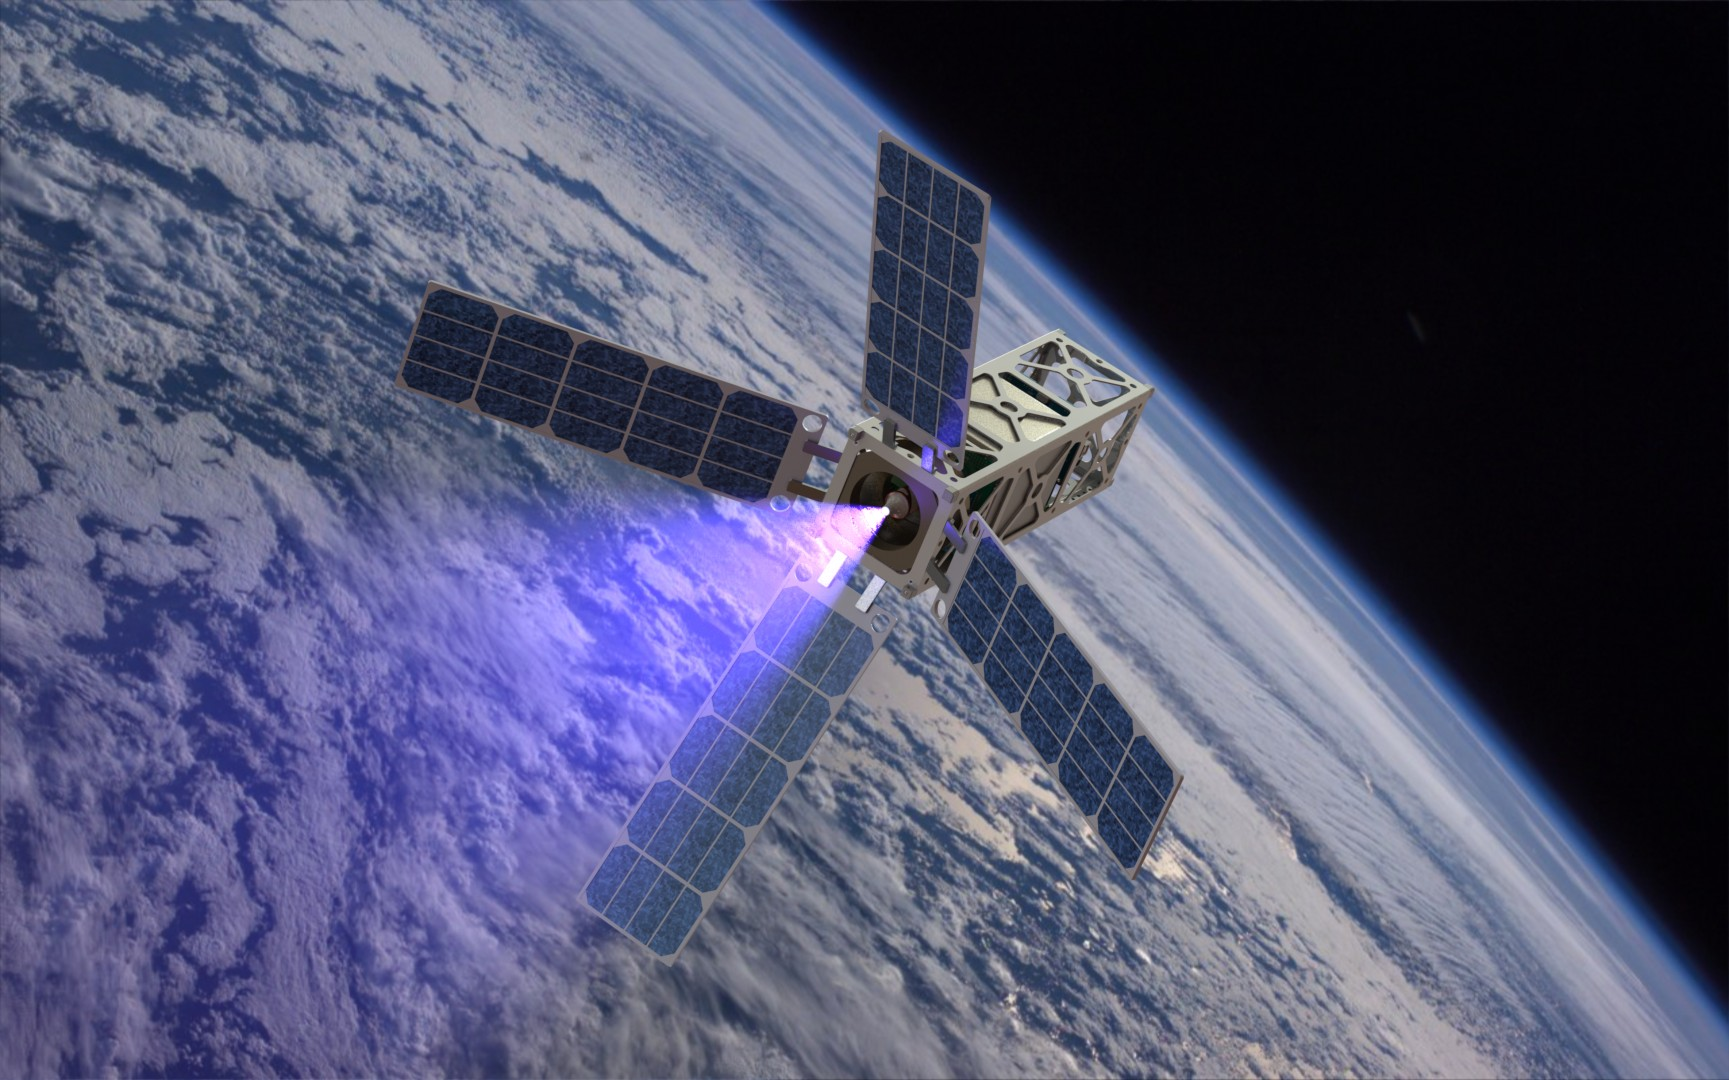
\includegraphics[height=0.4\textheight,width=0.5\textwidth,keepaspectratio]{figures/defense/patriot_plume.jpg}
    ~
    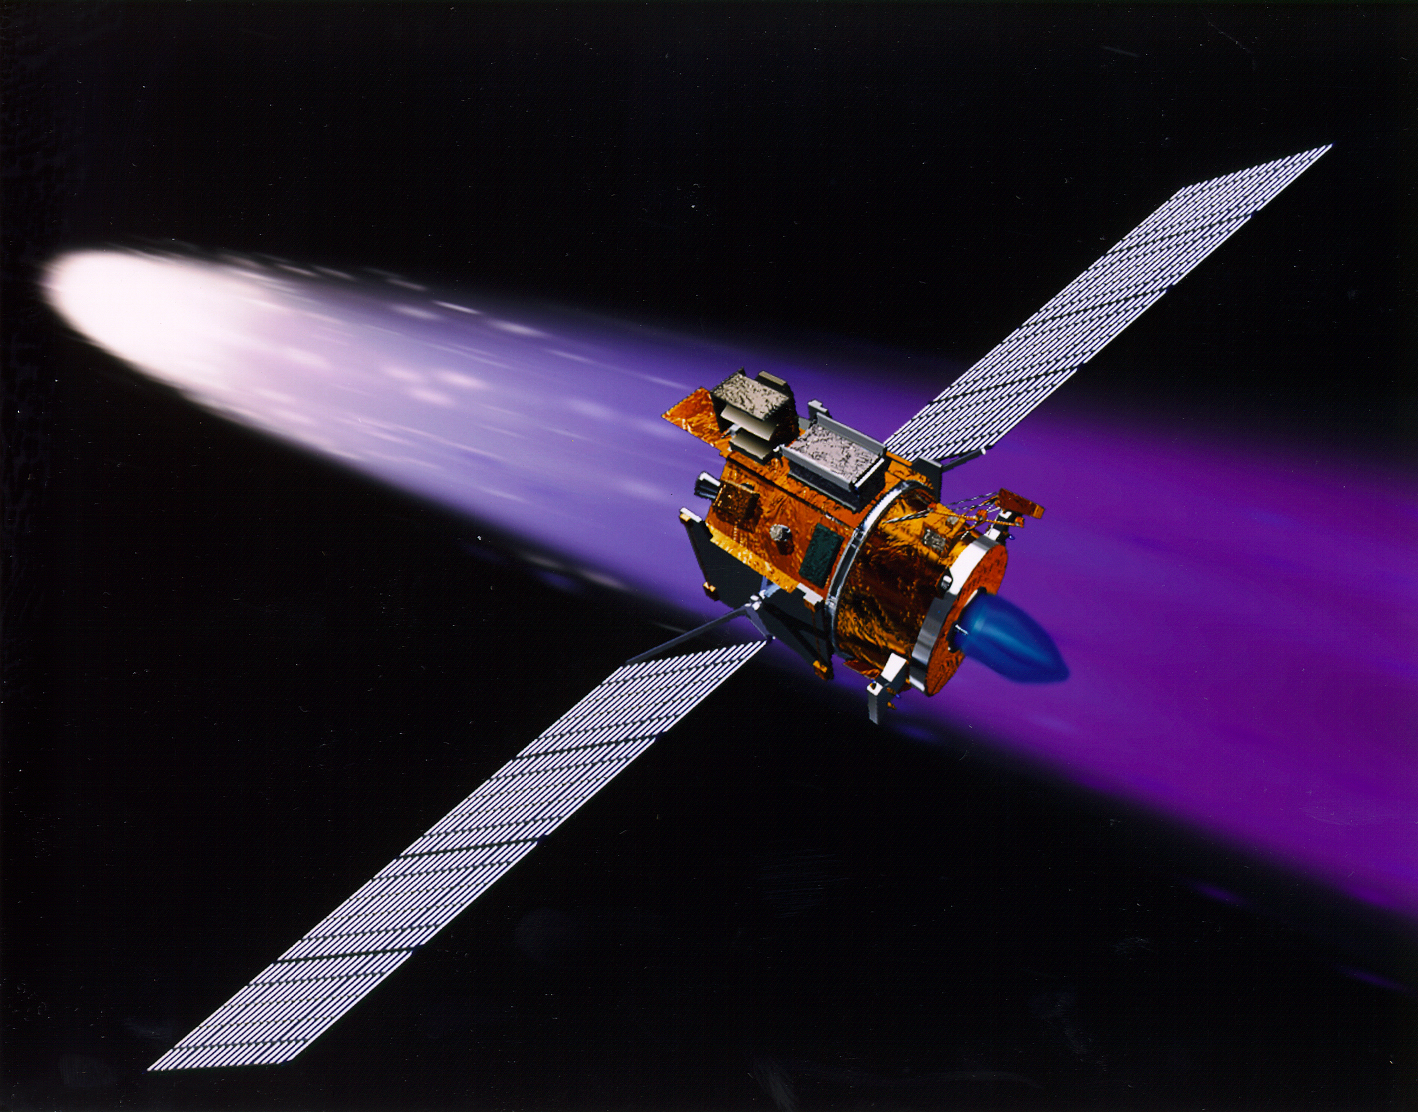
\includegraphics[height=0.4\textheight,width=0.5\textwidth,keepaspectratio]{figures/defense/deepspace1.jpg}
\end{center}
\hyperlink{slide:propulsion}{\beamergotobutton{Ideal Rockets}}
\end{frame}   %-----------------------------%

\begin{frame}{Low Thrust Orbital Transfers} % -----------------------------------%
    \begin{itemize}
        \item Low Thrust orbital transfers using reachability sets 
        \begin{itemize}
            \item Transfer design on lower dimensional \Poincare surface
            \item Simple method to incorporate effects of low-thrust 
            \item Avoids the issue of determining initial conditions
        \end{itemize}
    \pause
        \item Alleviates many issues with previous approaches
        \begin{itemize}
            \item Initial states chosen from from the reachable set
            \item Indirect optimal control vs. direct optimal control
            \item Reachability set gives bounds on motion
        \end{itemize}    
    \end{itemize}

  \note[itemize]{
    \item here we introduce some of our previous work that aims to apply geometric mechanics to the design of trajectories around asteroids
    \item Reachability set avoids the need to pick initial conditions
    \item We compute on a lower dimensional surface
  }
\end{frame} %--------------------------------------%

\subsection{Reachability on \Poincare Section}

\begin{frame}{\Poincare map}
\begin{itemize}
    \item Intersection of a periodic orbit with a lower dimensional subspace
    \pause
        \begin{itemize}
            \item  \Emph{\Poincare section} - discrete map between intersections
        \end{itemize}
        \pause
    \item Useful for investigating the stability and structure 
    \pause
    \item Define a \Poincare section \( \Sigma \) 
        \begin{itemize}
            \item Used for initial and target periodic orbits
            \item Subspace for the \Emph{reachability set}
        \end{itemize}
\end{itemize}

\begin{center}
    \resizebox{!}{0.5\textheight}{%
        \tikzsetnextfilename{poincare_map}
\tdplotsetmaincoords{60}{125} % view angle in spherical coordinates
\begin{tikzpicture}[
    tdplot_main_coords, 
    poincare/.style={opacity=.2,
    very thick,
    fill=blue},
    orbit/.style={very thick,black},
    orbit hidden/.style={very thick,dashed}, 
    grid/.style={very thin,gray!50},
    axis/.style={->,blue,thick},
    ]

    % nodes for the poincare section
    \node[label=above:\(\Sigma\)] (upper_right) at (0,5,5) {}; 
    \node[] (upper_left) at (0,1,5) {}; 
    \node[] (lower_left) at (0,1,0) {};
    \node[] (lower_right) at (0,5,0) {};

        % draw poincare section
    \draw[poincare] (upper_right.center) -- (upper_left.center) --
        (lower_left.center) -- (lower_right.center) --
        (upper_right.center);

        % draw a periodic orbit
    \coordinate (center) at (0,0,2); 
    \node[below right] (x0) at (0,2,2) {\(\vecbf{q}_0\)}; 
    \filldraw (0,2,2) circle (3pt);

    \node[below right] (x1) at (0,3,2) {\(\vecbf{q}_1\)};
    \filldraw (0,3,2) circle (3pt);

    \tdplotdrawarc[orbit hidden]{(center)}{2}{90}{190}{}{};
    \tdplotdrawarc[orbit,<-]{(center)}{2}{-170}{90}{}{};

    \tdplotdrawarc[orbit hidden]{(center)}{3}{90}{199}{}{};
    \tdplotdrawarc[orbit,<-]{(center)}{3}{-161}{90}{}{};

\end{tikzpicture}

    }
\end{center}

\note[itemize]{
    \item Here we present a review of the key components of dynamical systems theory
    \item we start with some initial condition \( {x}_0\) on a periodic orbit
    \item we then define a section \( \Sigma \) transverse to this flow
    \item we can use the successive iterations of these periodic orbits to study the dynamics of the system on a lower dimensional surface.
    \item Periodic orbits show up as fixed points while sinks/sources will have a distinctly different behavior
}
\end{frame}

\begin{frame}{Reachability Set}

\begin{itemize}
    \item Set of states achievable from a given initial condition over fixed \( t_f \) s.t. maximum control constraint
    \[
        R( \vc{x}_0, \mathcal{U} , t_f) = \braces{ \vc{x}_f \subseteq \mathcal{X} | \exists \vc{u} \in \mathcal{U}, \vc{x}(t_f) = \vc{x}_f }
    \]
    \pause
    \item Directly derivable from optimal control
    \item Frequently used for safety planning, e.g. air traffic avoidance
    \item We extend to the design of orbital transfers
\end{itemize}

\note[itemize]{
    \item Given the state of an aircraft, we can predict where it can end up over a fixed amount of time.
    \item To avoid any possibility of collision, we want to make sure these sets do not intersect
}
\end{frame}

\begin{frame}{Low Thrust Transfers via Reachability Sets } % -----------------------------------%

\begin{itemize}
    \item Generate the reachability set on a \Poincare section, \( \Sigma \)
    \item Control input is chosen to enlarge the reachable set
\end{itemize}

\begin{center}
    \resizebox{!}{0.8\textheight}{%
        \tdplotsetmaincoords{60}{125} % view angle in spherical coordinates
\begin{tikzpicture}[
    tdplot_main_coords,
    poincare/.style={opacity=.2,very thick,fill=blue},
    orbit/.style={very thick,black},
    orbit hidden/.style={very thick,dashed},
    grid/.style={very thin,black},
    axis/.style={->,blue,thick},
    reachability/.style={thick,blue},
    ]

        % nodes for the poincare section
    \node[label=above:\(\Sigma\)] (upper_right) at (0,5,5) {};
    \node[] (upper_left) at (0,1,5) {};
    \node[] (lower_left) at (0,1,0) {};
    \node[] (lower_right) at (0,5,0) {};

    % draw poincare section
    \draw[poincare] (upper_right.center) -- (upper_left.center) -- (lower_left.center) -- (lower_right.center) -- (upper_right.center);
    
    % draw a periodic orbit
    \coordinate (center) at (0,0,2);
    \node[label=below:\(\vecbf{x}_n\)] (x0) at (0,3,2) {};
    % \node[label=below:\(\vecbf{x}_n\)] at (x0) {};
    \filldraw (x0) circle (3pt);

    % \tdplotdrawarc[orbit hidden]{(center)}{3}{90}{200}{}{};
    \tdplotdrawarc[orbit,<-]{(center)}{3}{-160}{90}{}{};

    % draw reachability set on the poincare section
    \coordinate (reach) at (0,4.5,2);
    \tdplotsetthetaplanecoords{90}

    \draw[tdplot_rotated_coords,grid] (x0) -- (reach);
    \draw[tdplot_rotated_coords,grid] (x0) -- ++(-45:1.5);

    \tdplotdrawarc[tdplot_rotated_coords,grid]{(x0)}{0.5}{-45}{90}{above}{\(\theta_d\)};

    % draw terminal state on reachability set
    \node[tdplot_rotated_coords,label=above:\(\vecbf{x}_f\)] (xf) at ($ (x0)+(-45:1.5) $) {};
    \filldraw (xf) circle (3pt);

    \node[tdplot_rotated_coords,label=below:\(J\)] at (xf) {};

    \tdplotdrawarc[tdplot_rotated_coords,reachability]{(x0)}{1.5}{0}{360}{}{};
        % place
\end{tikzpicture}

    }
\end{center}

\note[itemize]{
    \item We combine both reachability and the \Poincare section to design transfers
    \item again we define our section \( \Sigma\)
    \item choose an initial state that is on \( \Sigma \)
    \item propogate without any control input from \( \vc{x}_0 \) to \( \vc{x}_n\)
    \item by adding the control input the terminal state will be something different at \( \vc{x}_f\)
    \item we define the distance between \( \vc{x}_n\) and \(\vc{x}_f\) with \( J \) - want to maximize this
    \item Repeat this computation many times for a variety of angles \( \phi\)
}
\end{frame} %--------------------------------------%

\subsection{Examples}
% show results of the transfer
\begin{frame}{Periodic Orbit Transfer}
    \begin{itemize}
        \item Transfer from periodic orbit to the Moon
        \item Orbit would provide constant line of site between Earth and far side
    \end{itemize}
    \begin{center}
        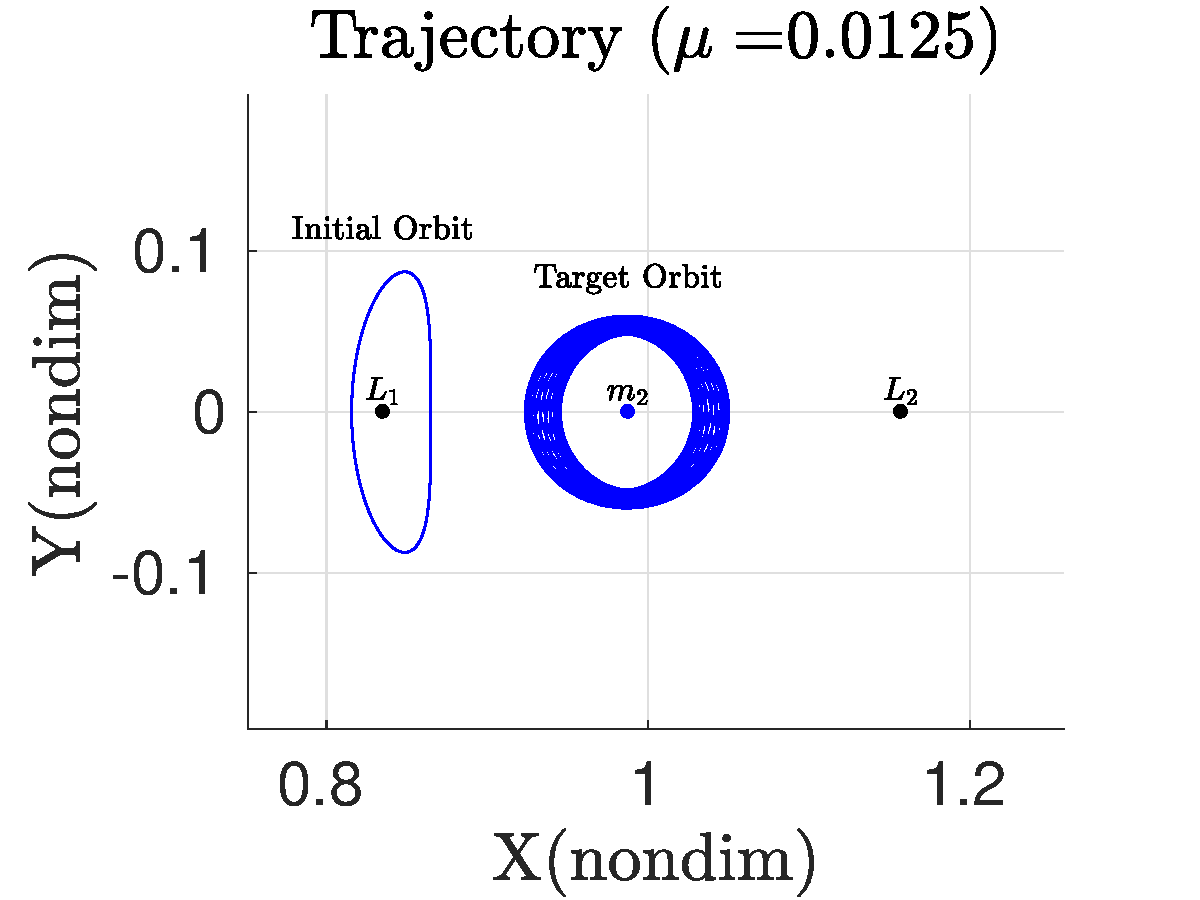
\includegraphics[height=0.75\textheight,keepaspectratio]{figures/2017_JAS/moon_orbit.pdf} % requires the graphicx package
   \end{center}
\end{frame}

\begin{frame}{Periodic Orbit Transfer}
    \begin{itemize}
        \item Reachable set is determined on the \Poincare section
        \item Intersection is used to determine the transfer
    \end{itemize}
    \begin{center}
        \only<1>{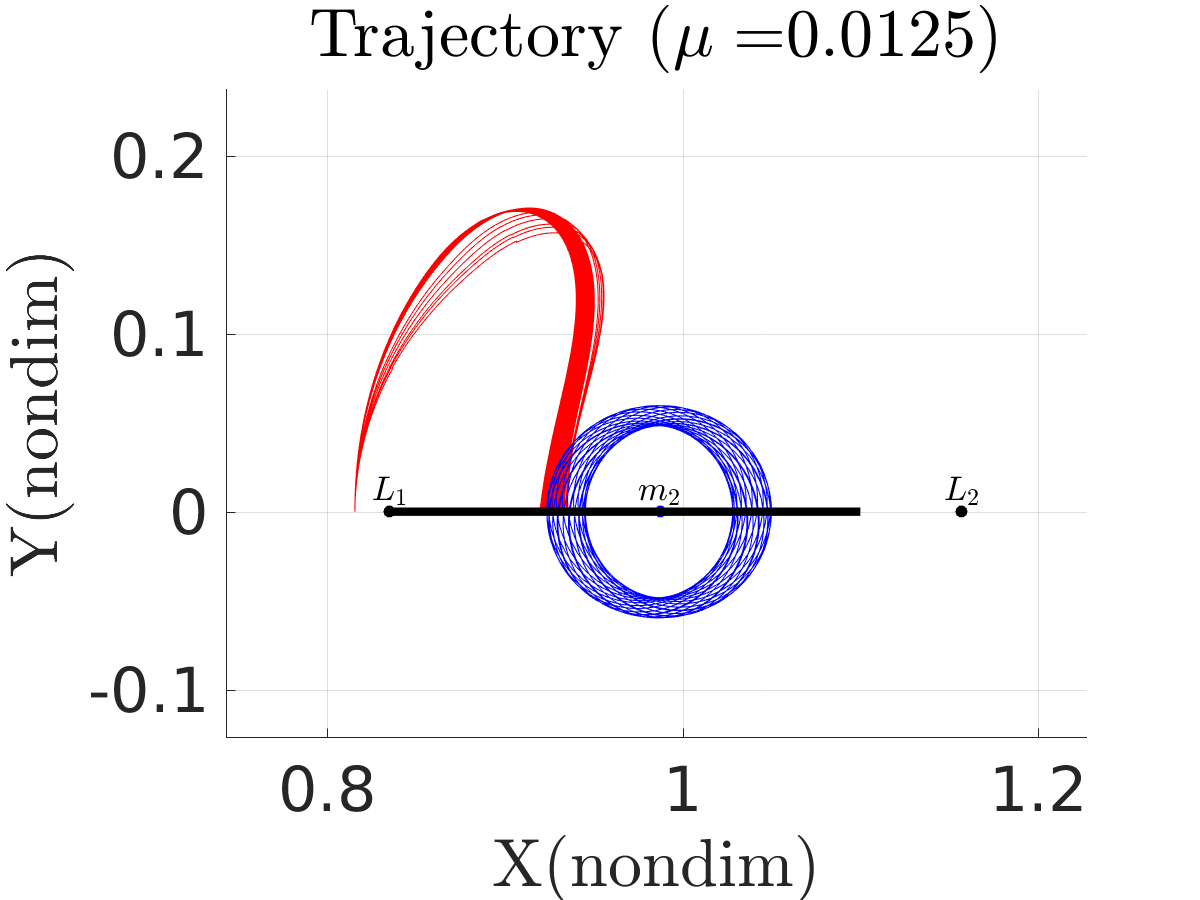
\includegraphics[width=0.5\textwidth]{figures/2017_JAS/reach_trajectory}}~
        \only<2>{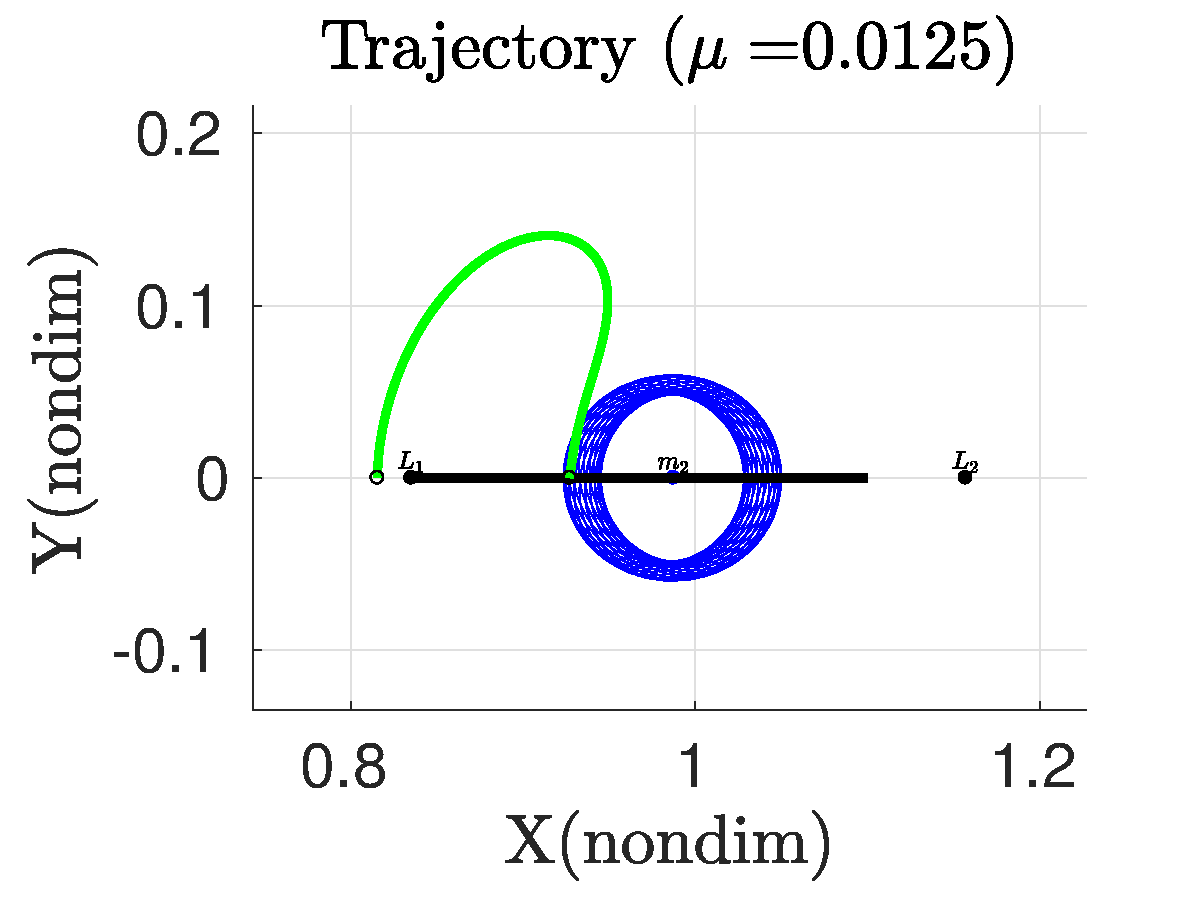
\includegraphics[width=0.5\textwidth]{figures/2017_JAS/reach_transfer.pdf}}~
        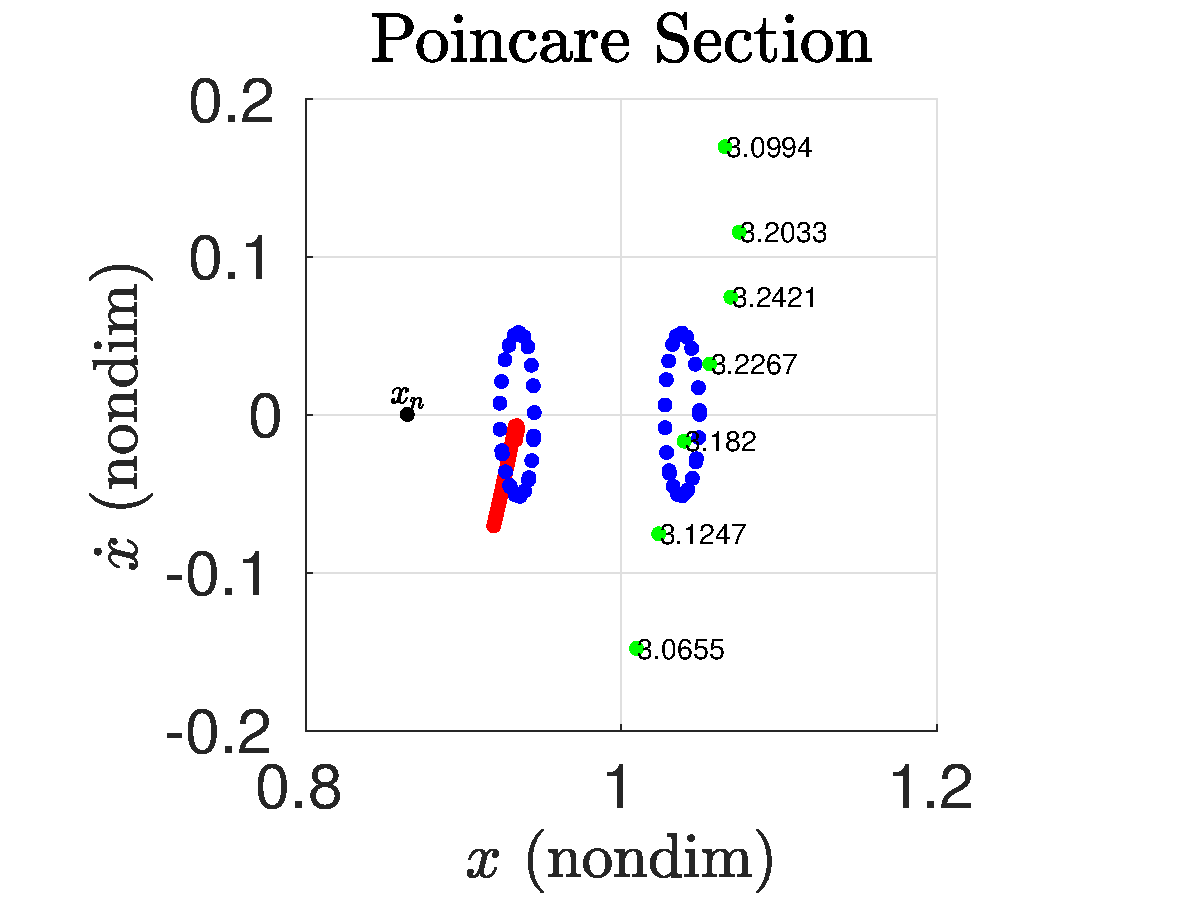
\includegraphics[width=0.5\textwidth]{figures/2017_JAS/poincare_compare} 
    \end{center}
\end{frame}

\begin{frame}{Geostationary Orbit Transfer}
    \begin{itemize}
        \item Now multiple reachable sets are combined for a larger transfer
        \item Transfer from geostationary to \( L_1 \) stable manifold
    \end{itemize}
    \begin{center}
            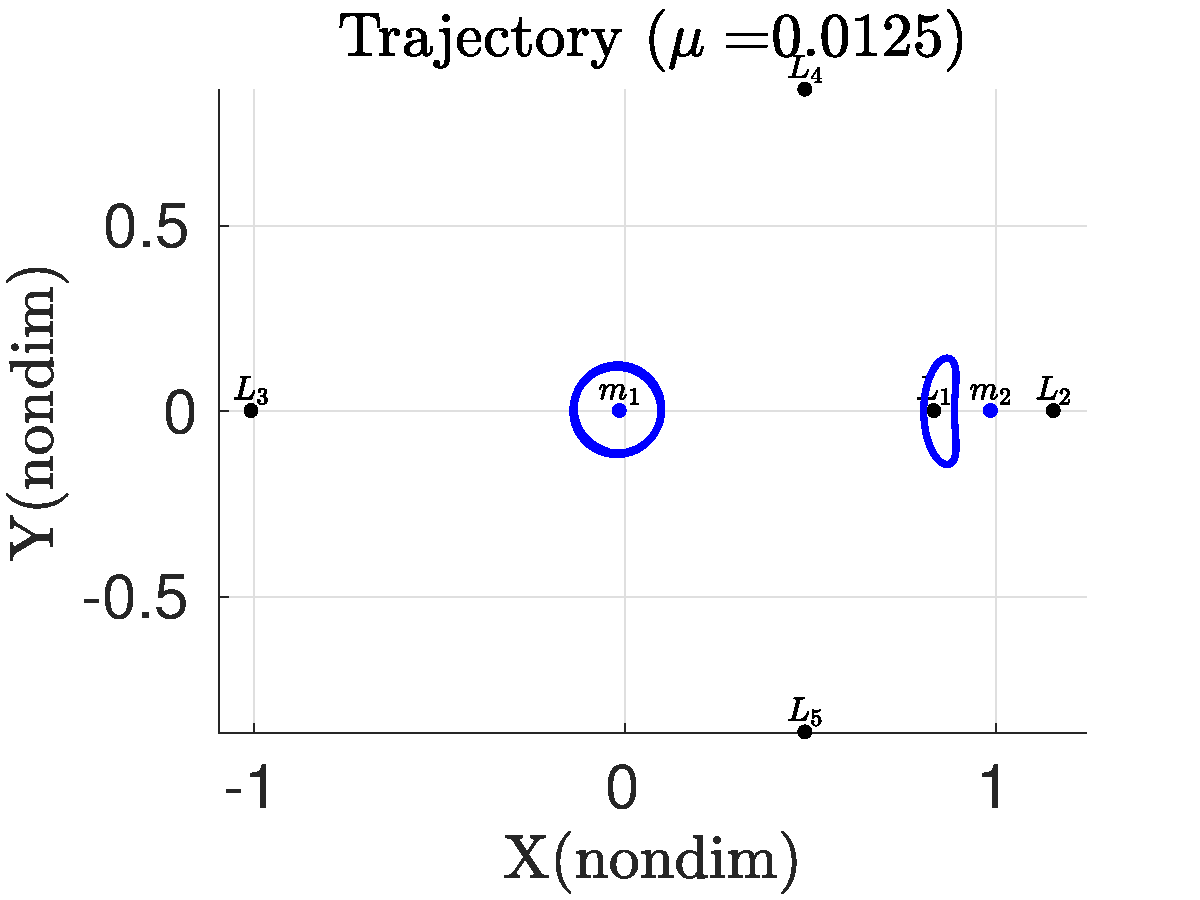
\includegraphics[height=0.8\textheight]{figures/2017_JAS/initial_final} % requires the graphicx package
    \end{center}
\end{frame}

\begin{frame}{Geostationary Orbit Transfer}
    \begin{itemize}
        \item Multiple reachability sets are linked to generate a transfer
    \end{itemize}
    \begin{center}
        \only<1>{
        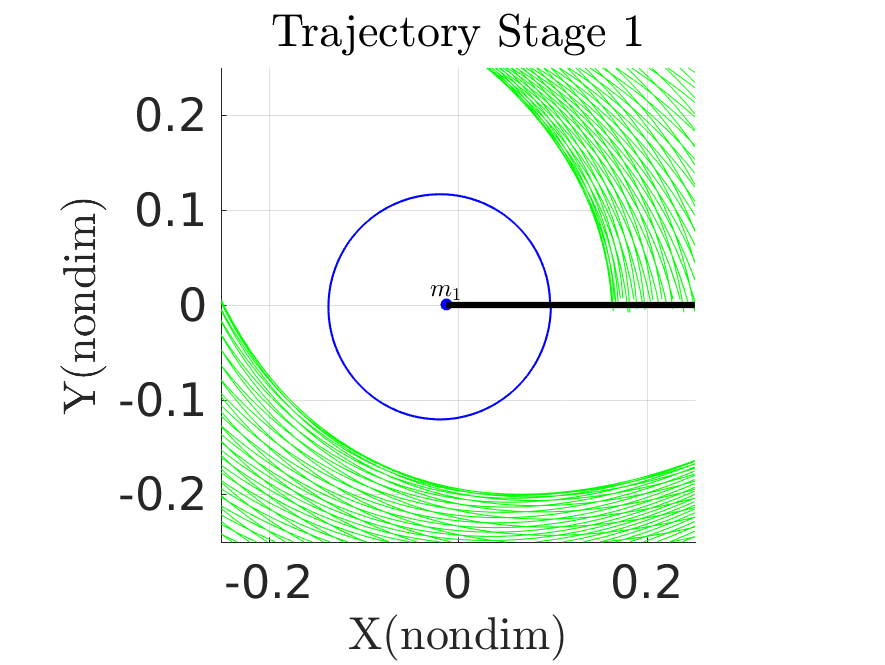
\includegraphics[height=0.8\textheight,width=0.5\textwidth,keepaspectratio]{figures/2017_JAS/stage1_trajectory_zoom.pdf}~
        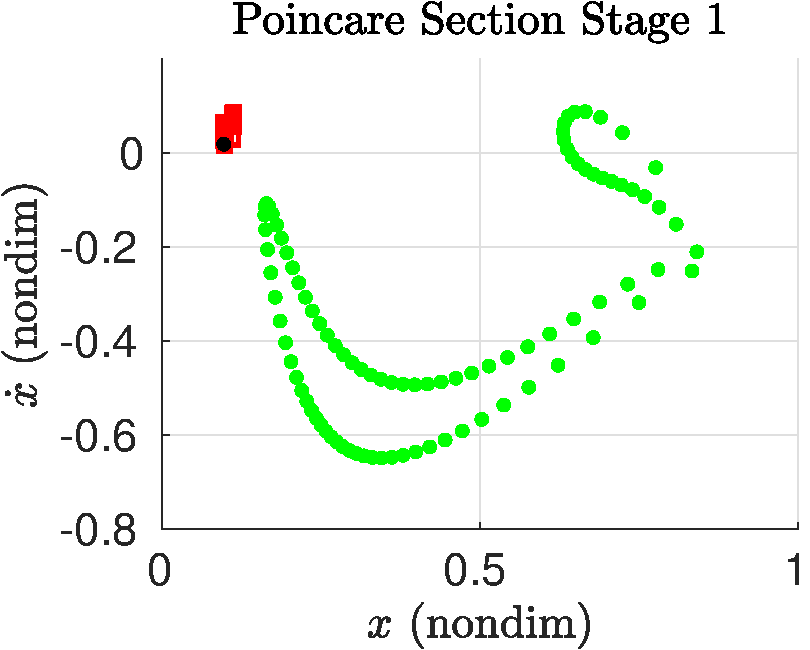
\includegraphics[height=0.8\textheight,width=0.5\textwidth,keepaspectratio]{figures/2017_JAS/stage1_poincare.pdf}
    }
        \only<2>{
        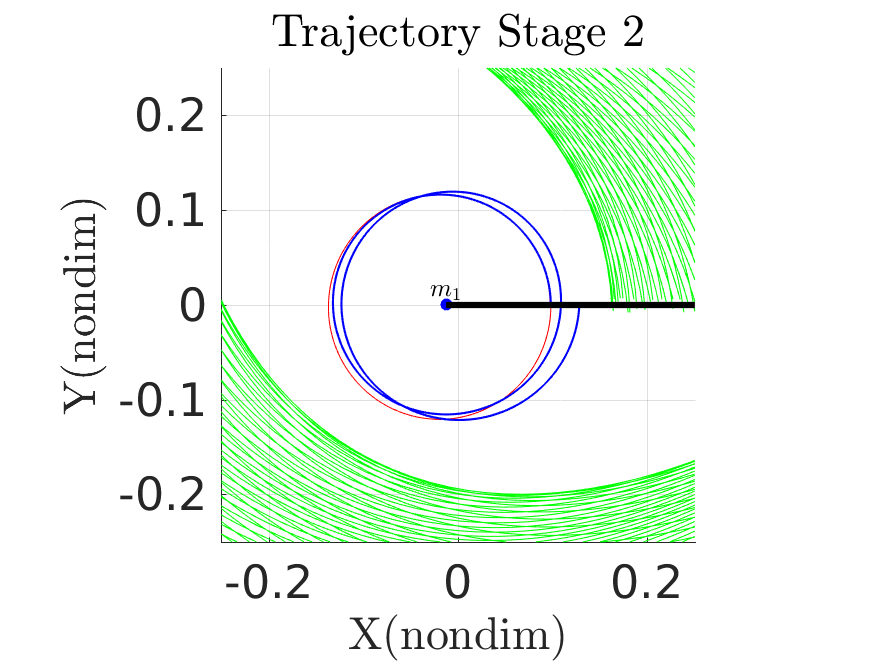
\includegraphics[height=0.8\textheight,width=0.5\textwidth,keepaspectratio]{figures/2017_JAS/stage2_trajectory_zoom.pdf}~
        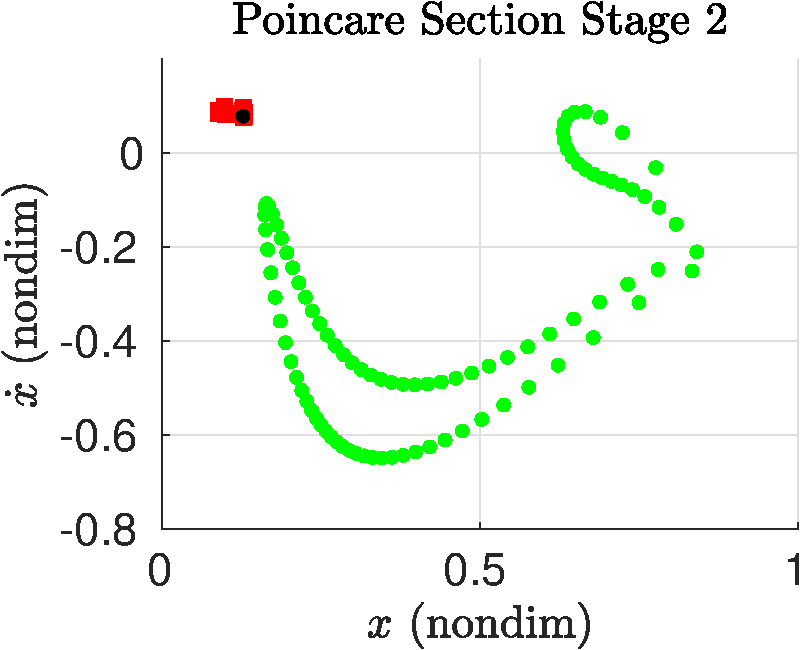
\includegraphics[height=0.8\textheight,width=0.5\textwidth,keepaspectratio]{figures/2017_JAS/stage2_poincare.pdf}
    }
        \only<3>{
        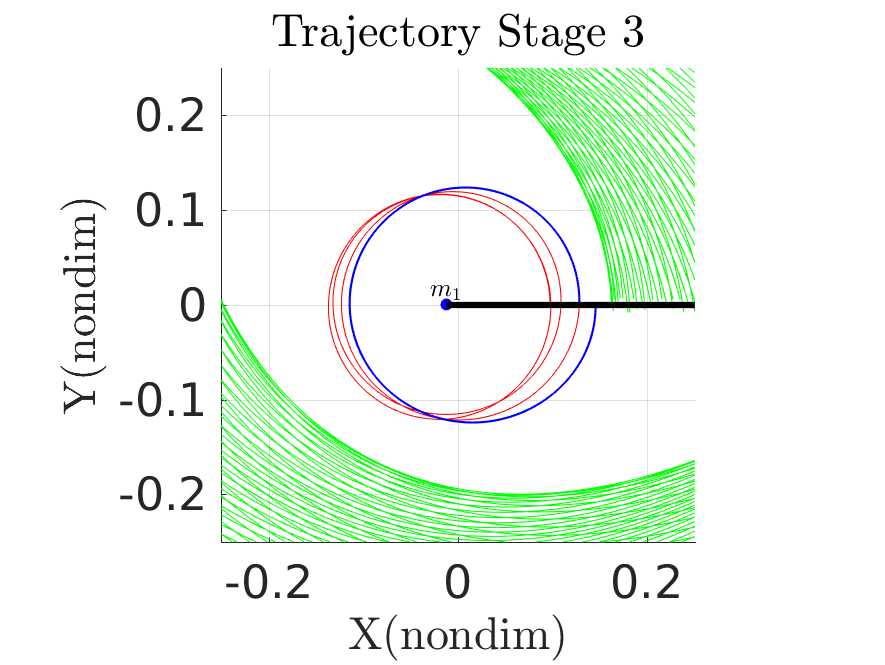
\includegraphics[height=0.8\textheight,width=0.5\textwidth,keepaspectratio]{figures/2017_JAS/stage3_trajectory_zoom.pdf}~
        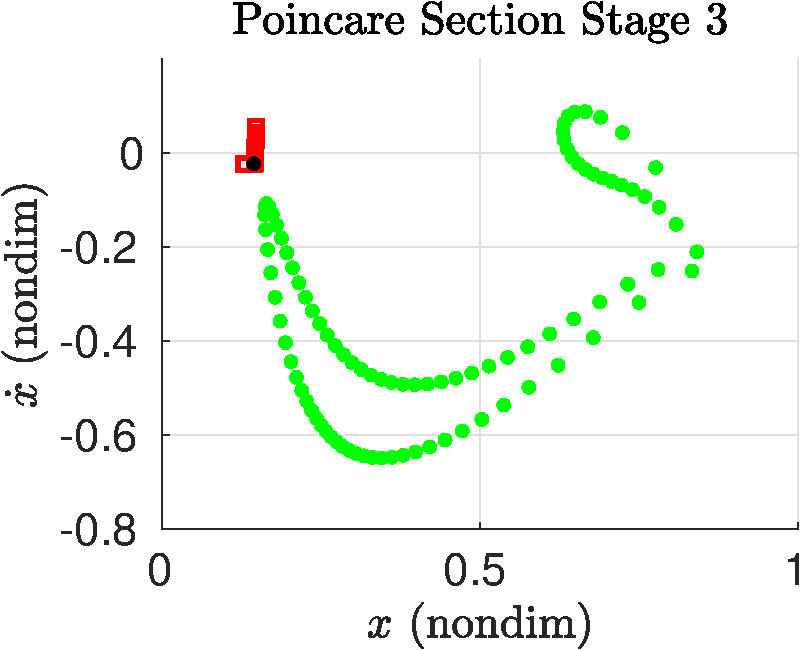
\includegraphics[height=0.8\textheight,width=0.5\textwidth,keepaspectratio]{figures/2017_JAS/stage3_poincare.pdf}
    }
        \only<4>{
        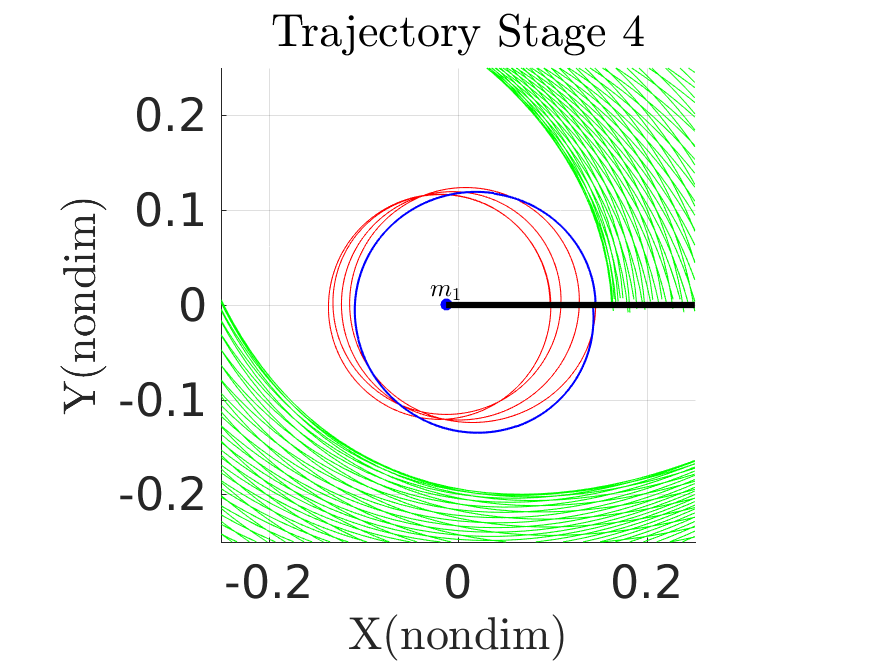
\includegraphics[height=0.8\textheight,width=0.5\textwidth,keepaspectratio]{figures/2017_JAS/stage4_trajectory_zoom.pdf}~
        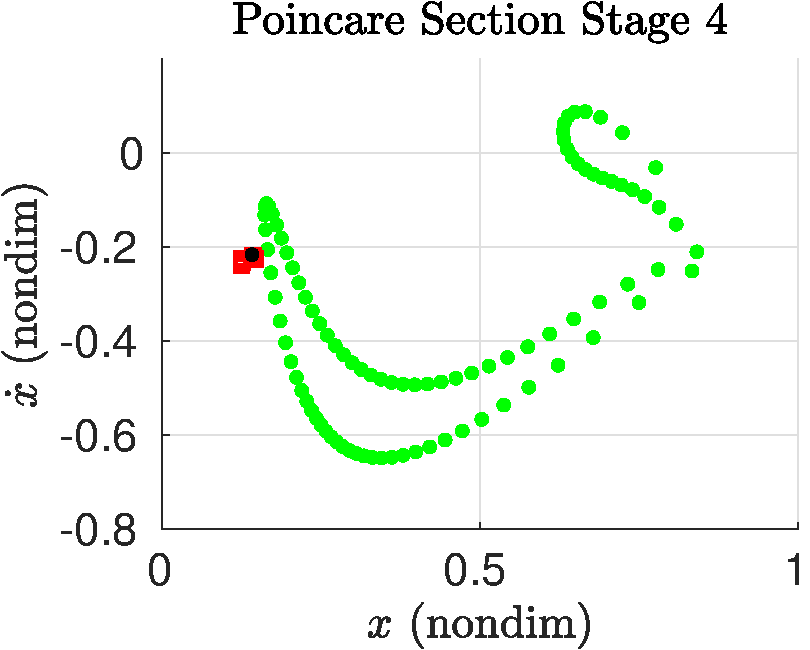
\includegraphics[height=0.8\textheight,width=0.5\textwidth,keepaspectratio]{figures/2017_JAS/stage4_poincare.pdf}
    }
        \only<5>{
        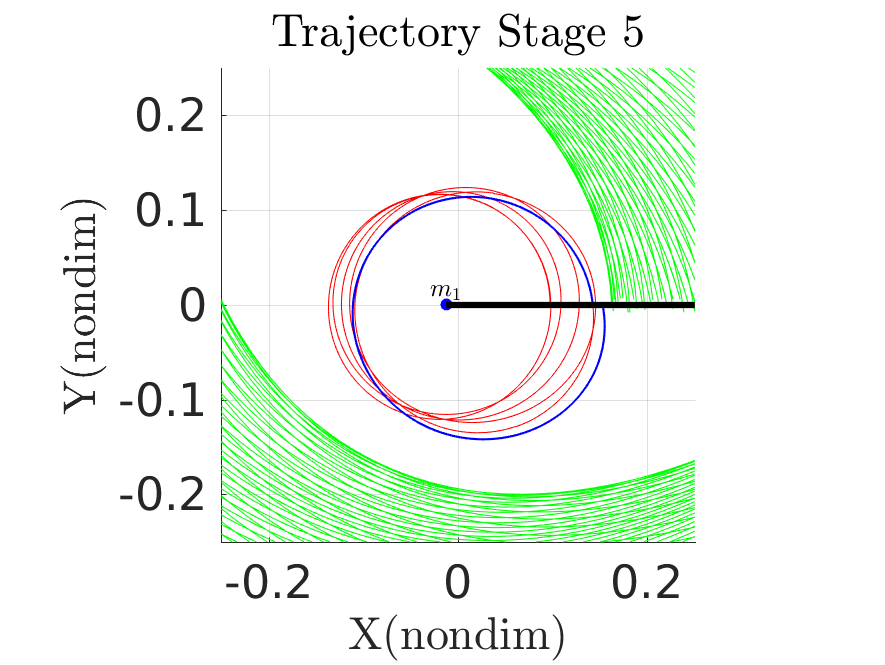
\includegraphics[height=0.8\textheight,width=0.5\textwidth,keepaspectratio]{figures/2017_JAS/stage5_trajectory_zoom.pdf}~
        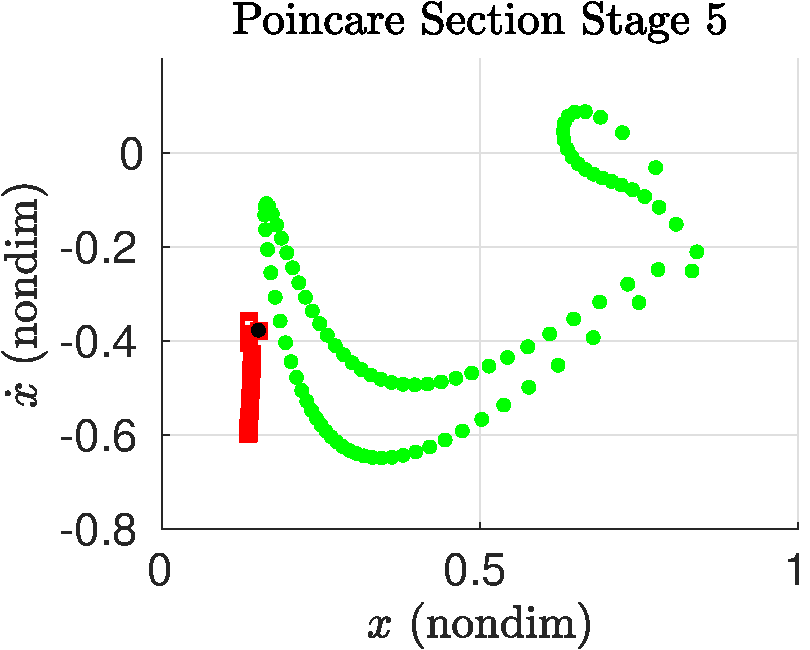
\includegraphics[height=0.8\textheight,width=0.5\textwidth,keepaspectratio]{figures/2017_JAS/stage5_poincare.pdf}
    }
        \only<6>{
        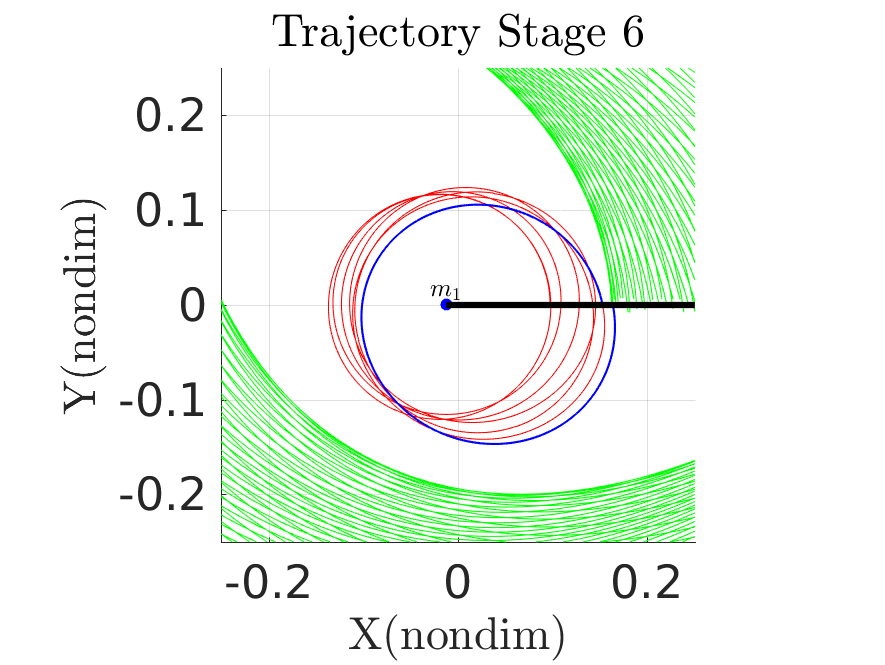
\includegraphics[height=0.8\textheight,width=0.5\textwidth,keepaspectratio]{figures/2017_JAS/stage6_trajectory_zoom.pdf}~
        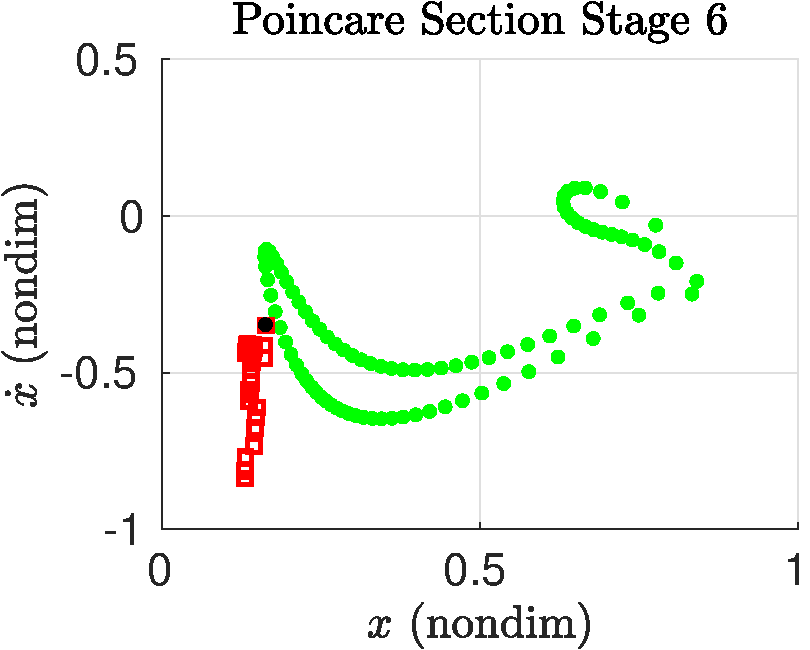
\includegraphics[height=0.8\textheight,width=0.5\textwidth,keepaspectratio]{figures/2017_JAS/stage6_poincare.pdf}
    }
        \only<7>{
        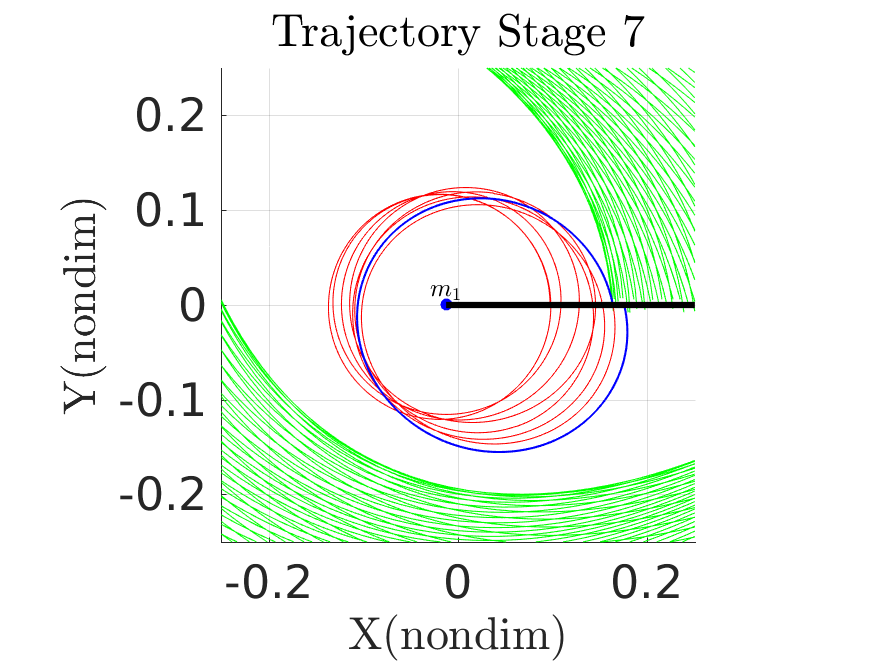
\includegraphics[height=0.8\textheight,width=0.5\textwidth,keepaspectratio]{figures/2017_JAS/stage7_trajectory_zoom.pdf}~
        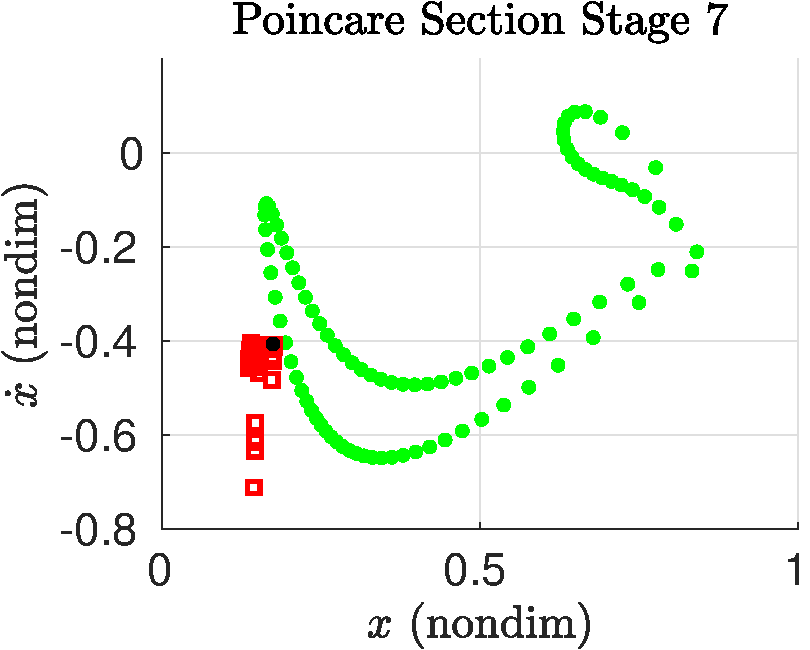
\includegraphics[height=0.8\textheight,width=0.5\textwidth,keepaspectratio]{figures/2017_JAS/stage7_poincare.pdf}
    }
        \only<8>{
        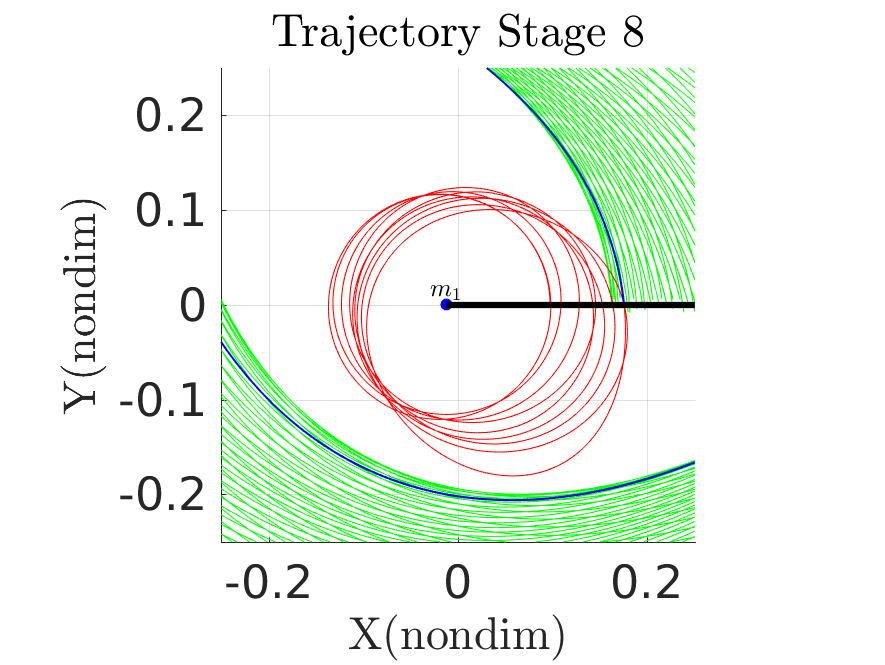
\includegraphics[height=0.8\textheight,width=0.5\textwidth,keepaspectratio]{figures/2017_JAS/stage8_trajectory_zoom.pdf}~
        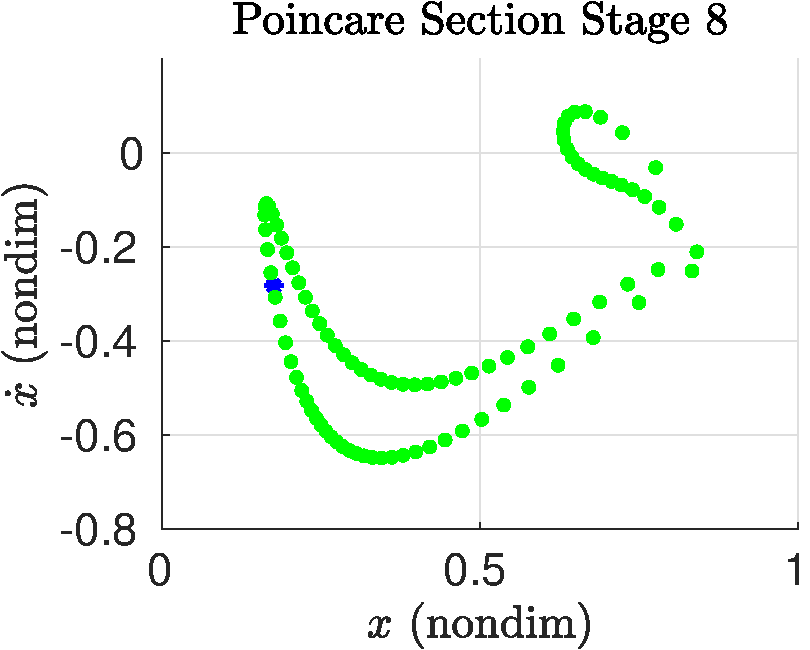
\includegraphics[height=0.8\textheight,width=0.5\textwidth,keepaspectratio]{figures/2017_JAS/stage8_poincare.pdf}
    }
    \only<9>{
        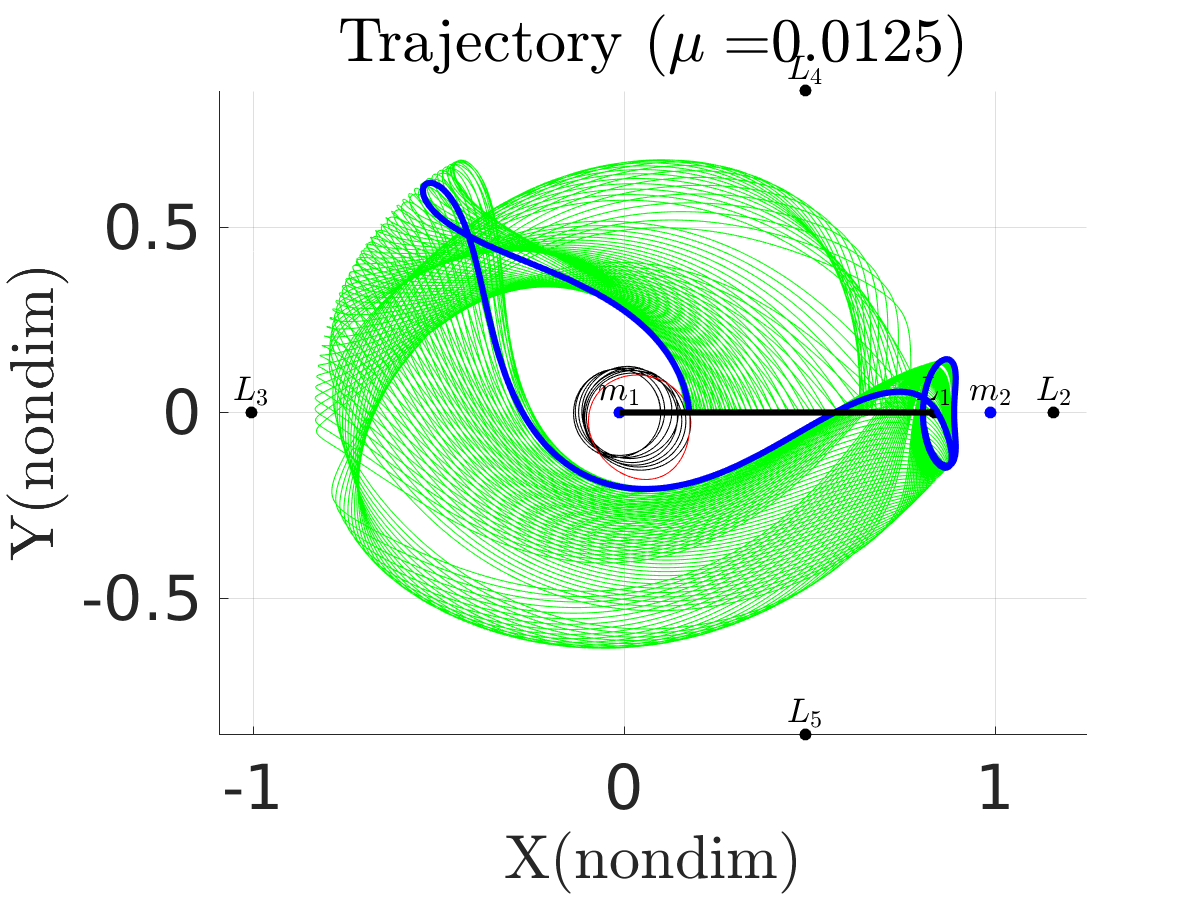
\includegraphics[width=0.45\textwidth]{figures/2017_JAS/geo_transfer_full}~
        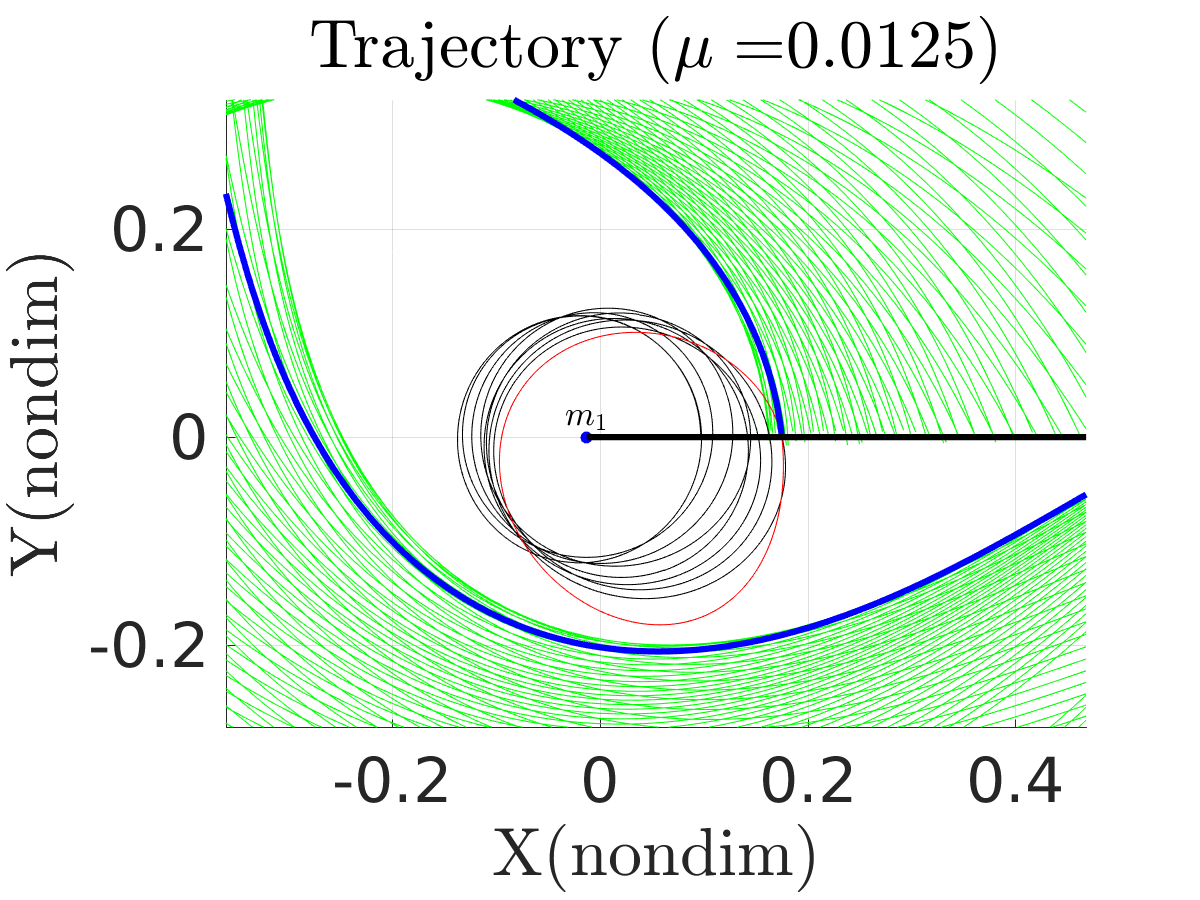
\includegraphics[width=0.45\textwidth]{figures/2017_JAS/geo_transfer_zoom}
    }
    \end{center}
\end{frame}

\begin{frame}{4769 Castalia Transfer}
    \begin{itemize}
        \item Extend the transfer to full 3D case around an asteroid
        \item Reachability set is now four dimensional
    \end{itemize}
    \begin{center}
        \only<1>{
        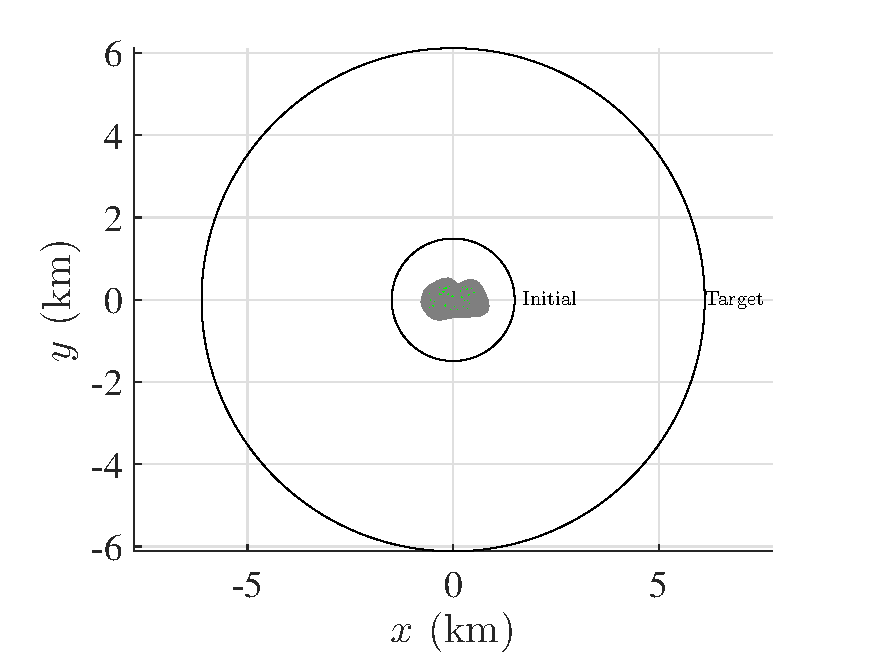
\includegraphics[width=0.5\textwidth]{figures/2016_AAS/initial_transfer}~
        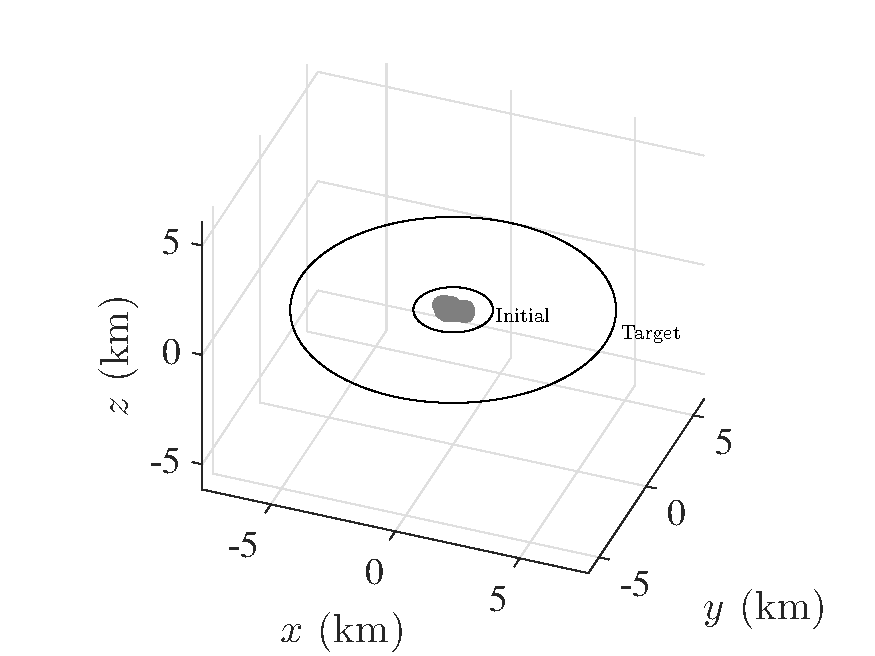
\includegraphics[width=0.5\textwidth]{figures/2016_AAS/initial_transfer_3d} 
    }
    \only<2>{
        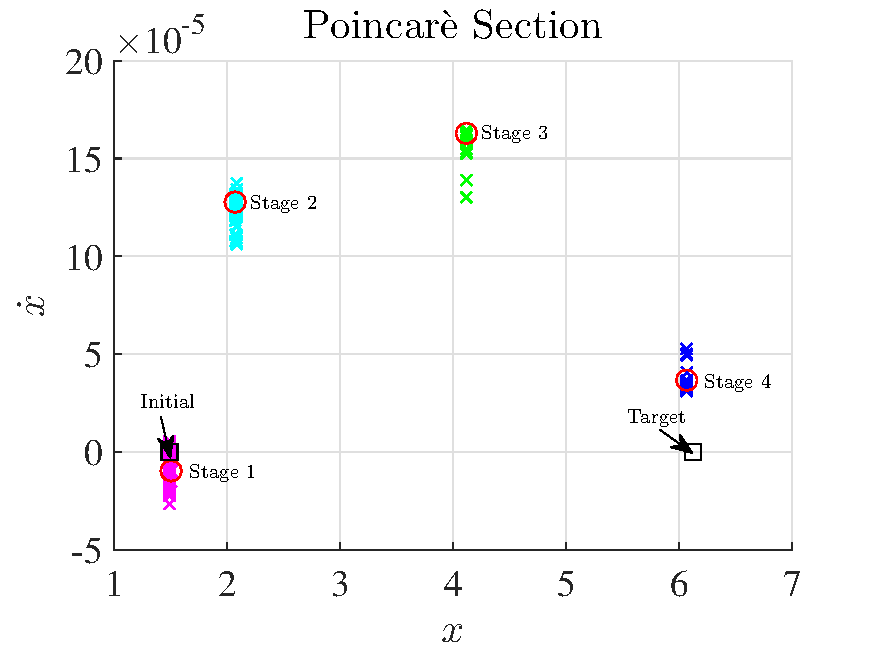
\includegraphics[width=0.5\textwidth]{figures/2016_AAS/poincare_xvsxdot.pdf}~
        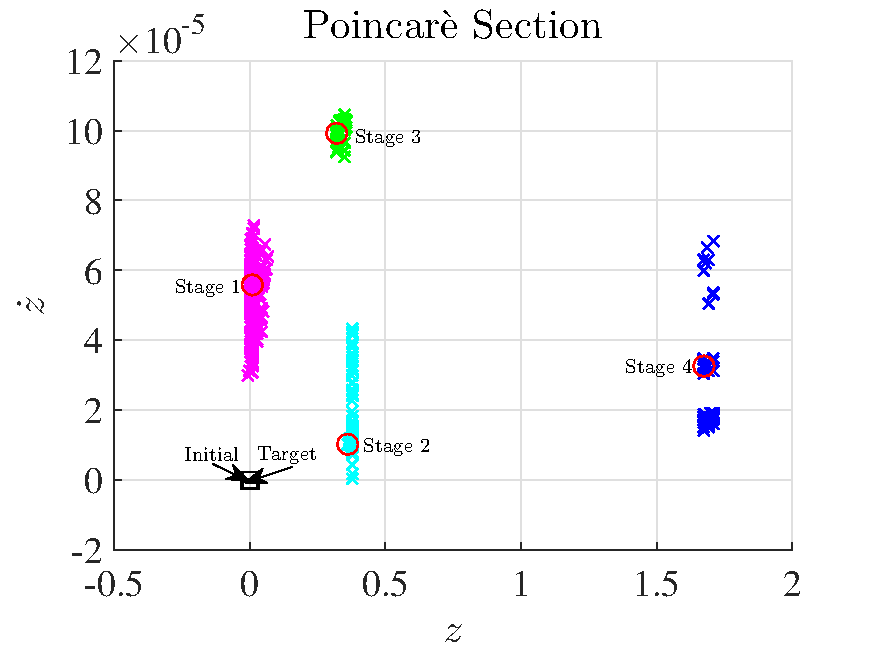
\includegraphics[width=0.5\textwidth]{figures/2016_AAS/poincare_zvszdot.pdf} 
    }
    \only<3>{
        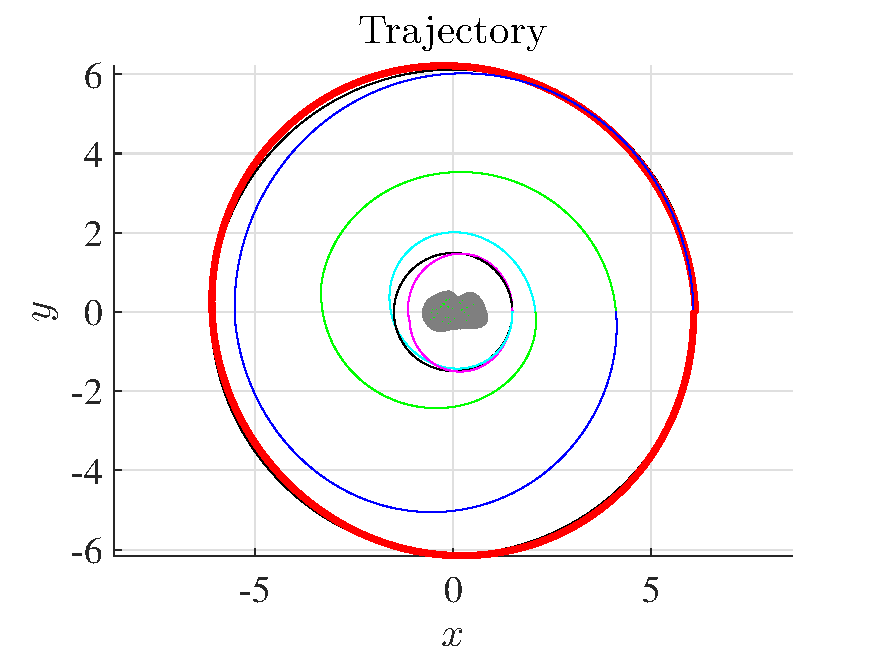
\includegraphics[width=0.5\textwidth]{figures/2016_AAS/trajectory.pdf}~
        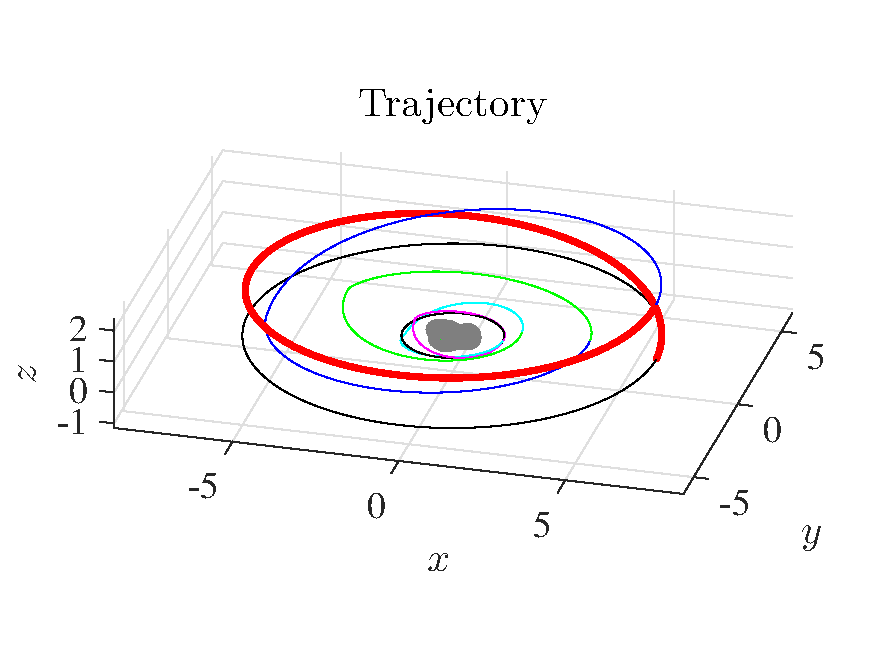
\includegraphics[width=0.5\textwidth]{figures/2016_AAS/trajectory_3d.pdf} 
    }
    \end{center}
\end{frame}

% !TEX root = ../../defense.tex

\section{Geometric Control}

\begin{frame}{Geometric Control}
    \begin{itemize}
        \item Extension of control design to differentiable manifolds
            \begin{itemize}
                \item A set which locally ``looks'' like Euclidean space
                \item More general as the techniques are no longer limited to vector spaces
            \end{itemize}
        \item Analysis is ``coordinate-free'' or ``intrinsic''
            \begin{itemize}
                \item The choice of coordinates should not bias the dynamics/control 
            \end{itemize}
        \item Mathematically precise method to derive dynamics and control laws that faithfully represent the system
            \begin{itemize}
                \item Identification of the configuration manifold, \( \SO \)
                \item Choose a coordinate representation, \( R \in \SO \)
                \item Dynamics: Derive kinetic and potential energies as function of coordinates
                \item Control: Configuration error as function of coordinates
                \item Determine control input to stabilize about desired state/trajectory
            \end{itemize}
    \end{itemize}
\end{frame}
\subsection[Spacecraft Autonomy]{Spacecraft Autonomy}
% why study the coupled attitude/translational problem

\begin{frame}[t]{Spacecraft Autonomy} %-----------------------------%
\begin{itemize}
    \item Autonomous control of space vehicles is critical
    \begin{itemize}
        \item Avoid extensive planning and interaction by operators
        \item Ability to operate safely with system uncertainty 
        \item Independently navigate hazards and handle possible failures
    \end{itemize}
\end{itemize}
\visible<2>{
\begin{center}
    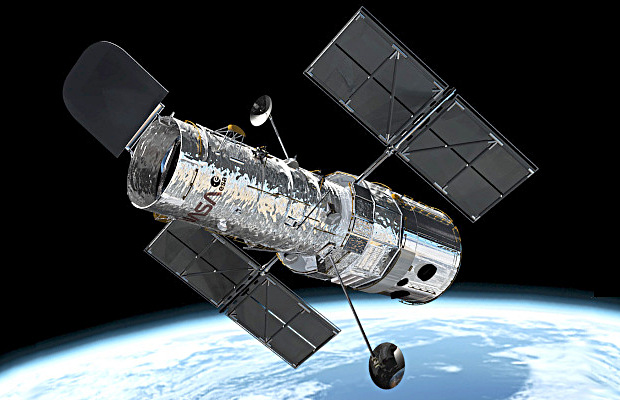
\includegraphics[width=0.5\textwidth,height=0.35\textheight,keepaspectratio]{figures/defense/hubble.jpg}\hfill
    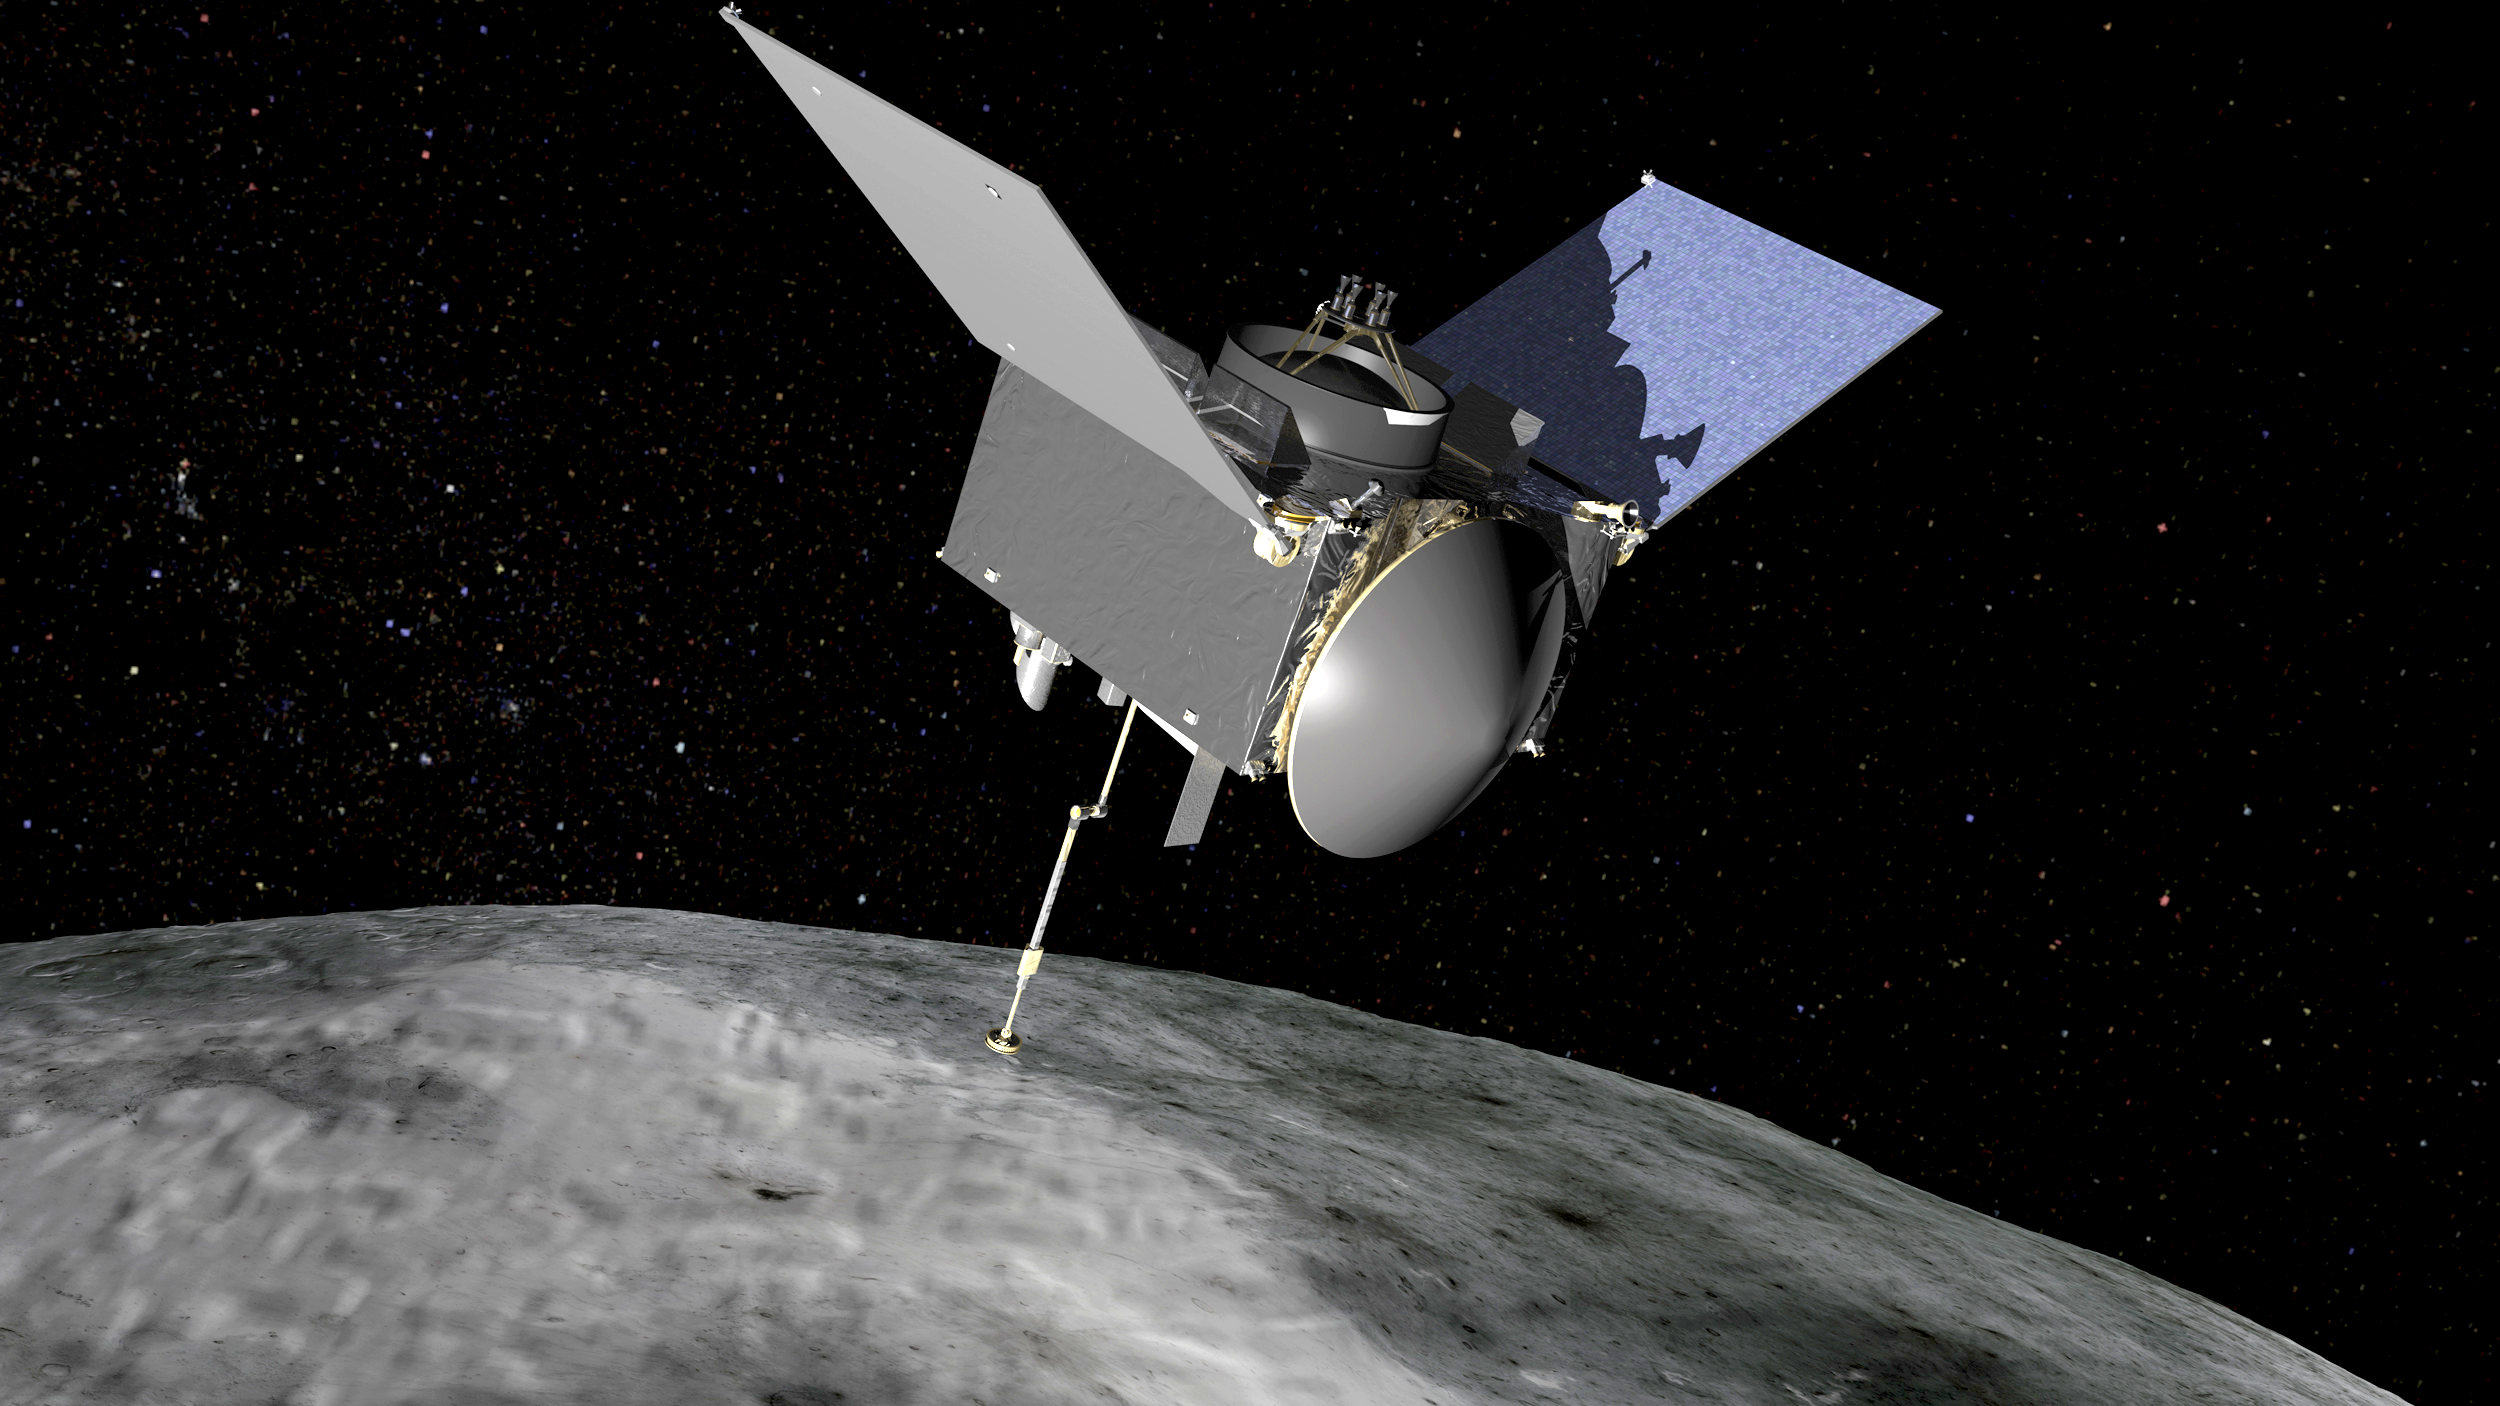
\includegraphics[width=0.5\textwidth,height=0.4\textheight,keepaspectratio]{figures/defense/osires_rex.png}
\end{center}
}
\note[itemize]{
    \item Autonomy is a key component to enable asteroid missions
}
\end{frame}   %-----------------------------%


\subsection{Attitude Control}

\begin{frame}[t]{Problem Formulation} %-----------------------------------%
\begin{itemize}
    \item \Emph{Constrained attitude control} : reorient vehicle while avoiding pointing at obstacles
    \begin{itemize}
        \item Exclusion zones for payloads e.g infrared telescope
        \item UAVs manuevering in congested locations
        \item Laser/Radio emitters on spacecraft
    \end{itemize}
    \pause
    \item Previous approaches have several issues
    \begin{itemize}
        \item Attitude parameterizations: singularities/ambiguities
        \item Ad-hoc path planning: difficult to generalize to arbitrary obstacles
        \item Randomized methods: lack of stability guarantees
        \item Optimization based: expensive to compute and only provides open-loop control  
    \end{itemize}
\end{itemize}
\end{frame} %-------------------------------------%

\begin{frame}{Attitude Parameterizations}
    \begin{itemize}
        \item Euler Angles
        \begin{itemize}
            \item Minimal representation used for small attitude changes.
            \item Singularities exist for large angle slews: requires switching between 24 sequences
            \item Complicated trigonometric functions
        \end{itemize}
        \pause
        \item Quaternion 
        \begin{itemize}
            \item No singularities
            \item Two anti-podal quaternions for the same attitude
            \item Unwinding behavior for control systems
        \end{itemize}
        \pause
        \item Geometric control
        \begin{itemize}
            \item Globally and uniquely characterize attitude: \( R \in \SO \)
            \item Controller is globally valid for large angle maneuvers
        \end{itemize}
    \end{itemize}
    
\end{frame}

\begin{frame}{Objective} %---------------------------------------%

    \begin{block}{Nonlinear Control Design}
        Design control input \( u \) that stabilizes system from initial attitude \( R_0 \) to desired attitude \( R_d \) while avoiding obstacles
    \end{block}
    \pause
    \begin{itemize}
        \item Avoid drawbacks of other approaches 
        \begin{itemize}
            \item \Emph{Geometric control} - analysis is conducted directly on \( \SO \) 
            \item \Emph{Barrier function} - allows for arbitrary amount of constraints
            \item \Emph{Efficient } - real time feedback control
            \item \Emph{Stability} - Lyapunov analysis gives rigourous stability proof
            \item \Emph{Adaptive} - handles system uncertainties
        \end{itemize}
    \end{itemize}
\end{frame}


\begin{frame}{Spacecraft Orientation} %-----------------------------%

\begin{itemize}

    \item \Emph{Attitude Representation}: rotation matrix from body to inertial frame
     \[\SO =  \{R\in\R^{3\times 3}\,|\, R^TR=I,\;\mathrm{det}[R]=1\} . \]
    \item Rigid body attitude dynamics:
    \begin{gather*}
        J\dot\Omega + \Omega\times J\Omega = u+W(R,\Omega)\Delta , \quad \dot R = R\hat\Omega .
    \end{gather*}

    \item Sensor and obstacles defined by unit vectors in \( \R^3 \) 
        \begin{itemize}
            \item Body fixed sensor: \( r \in \S^2\)
            \item Inertially fixed hazard: \( v \in \S^2 \)
        \end{itemize} 
    \item Hard cone constraint: \( r^T R^T v \leq \cos \theta \)
    
\end{itemize}
\end{frame}   %-----------------------------%

\begin{frame}{Configuration Error Function} %-----------------------------%
\only<1>{
\begin{itemize}
    \item Error function quantifies ``distance'' to desired attitude
    \begin{align*}
            \Psi(R, R_d) = A(R, R_d) B(R) .
    \end{align*}
    \item Combination of attractive and repulsive terms   
\end{itemize}
\begin{gather*}
    A(R, R_d) = \frac{1}{2} \tr{G \left( I - R_d^T R\right)} . \\ \\
    B_i(R) = 1 - \frac{1}{\alpha_i} \ln \left( - \frac{ r^T R^T v_i - \cos \theta_i}{1 + \cos \theta_i}\right) .
\end{gather*}     
}

\only<2>{
    \begin{itemize}
        \item Attractive well at the desired attitude
    \end{itemize}
    \begin{align*}
        A(R,R_d) = \frac{1}{2} \tr{G \left( I - R_d^T R\right)} .
    \end{align*}
    \begin{center} 
        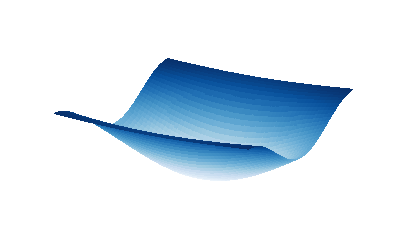
\includegraphics[height=0.8\textheight]{figures/2016_IJCAS/attract_error.pdf}
    \end{center}
}

\only<3>{
    \begin{itemize}
        \item Define a barrier around obstacles
    \end{itemize}
    \begin{align*}
        B_i(R) = 1 - \frac{1}{\alpha_i} \ln \left( - \frac{ r^T R^T v_i - \cos \theta_i}{1 + \cos \theta_i}\right).
    \end{align*}
    \begin{center}
        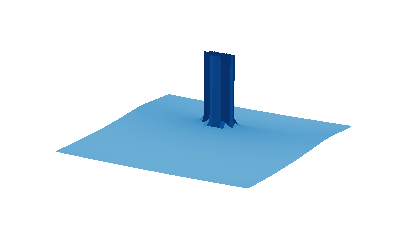
\includegraphics[height=0.8\textheight]{figures/2016_IJCAS/avoid_error.pdf}
    \end{center}

}

\only<4>{
    \begin{itemize}
        \item Configuration error: \( \Psi : \Q \times \Q \to \R \) with control chosen to follow slope of \( \Psi \) to minimum at \( R_d\)
    \end{itemize}
    \begin{align*}
        \Psi(R, R_d) = A(R,R_d) B(R) .
    \end{align*}
    \begin{center}
        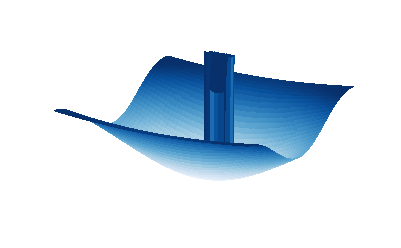
\includegraphics[height=0.8\textheight]{figures/2016_IJCAS/combined_error.pdf}
    \end{center}
}

\note[itemize]{
    \item First step in control design is the selection of an error function
}
\end{frame}   %-----------------------------%

\subsection{Examples}
\begin{frame}{Numerical Simulation} %-----------------------------%

\begin{itemize}
    \item Simulate a S/C completing a yaw rotation
    \item Single obstacle in the path of sensor
\end{itemize}

\begin{center}
    \animategraphics[controls,autoplay,loop,width=0.5\textwidth,height=0.7\textheight,keepaspectratio]{8}{animation/2016ACC/single_noavoid/single_noavoid-}{0}{99}~
    \animategraphics[controls,autoplay,loop,width=0.5\textwidth,height=0.7\textheight,keepaspectratio]{8}{animation/2016ACC/single_avoid/single_avoid-}{0}{99}
\end{center}

\end{frame}%-----------------------------%

\begin{frame}{Multiple Obstacles}%-------------------------------------%

\begin{itemize}
    \item Easily handle multiple arbitrary constraints 
    \begin{align*}
        \Psi = A(R) \bracket{1 + \sum_i C_i(R)} \quad C_i = B(R) - 1
    \end{align*}
\end{itemize}

\begin{center}
    \animategraphics[controls,autoplay,loop,width=0.5\textwidth,height=0.5\textheight,keepaspectratio]{8}{animation/2016ACC/multiple_avoid/multiple_avoid-}{0}{99}
\end{center}

\end{frame}%---------------------------------------%

\begin{frame}{Hexrotor Experiment} %-----------------------------%
\begin{itemize}
    \item Attached to spherical joint to allow only attitude dynamics
\end{itemize}
\begin{center}
    \href{https://youtu.be/dsmAbwQram4?t=20s}{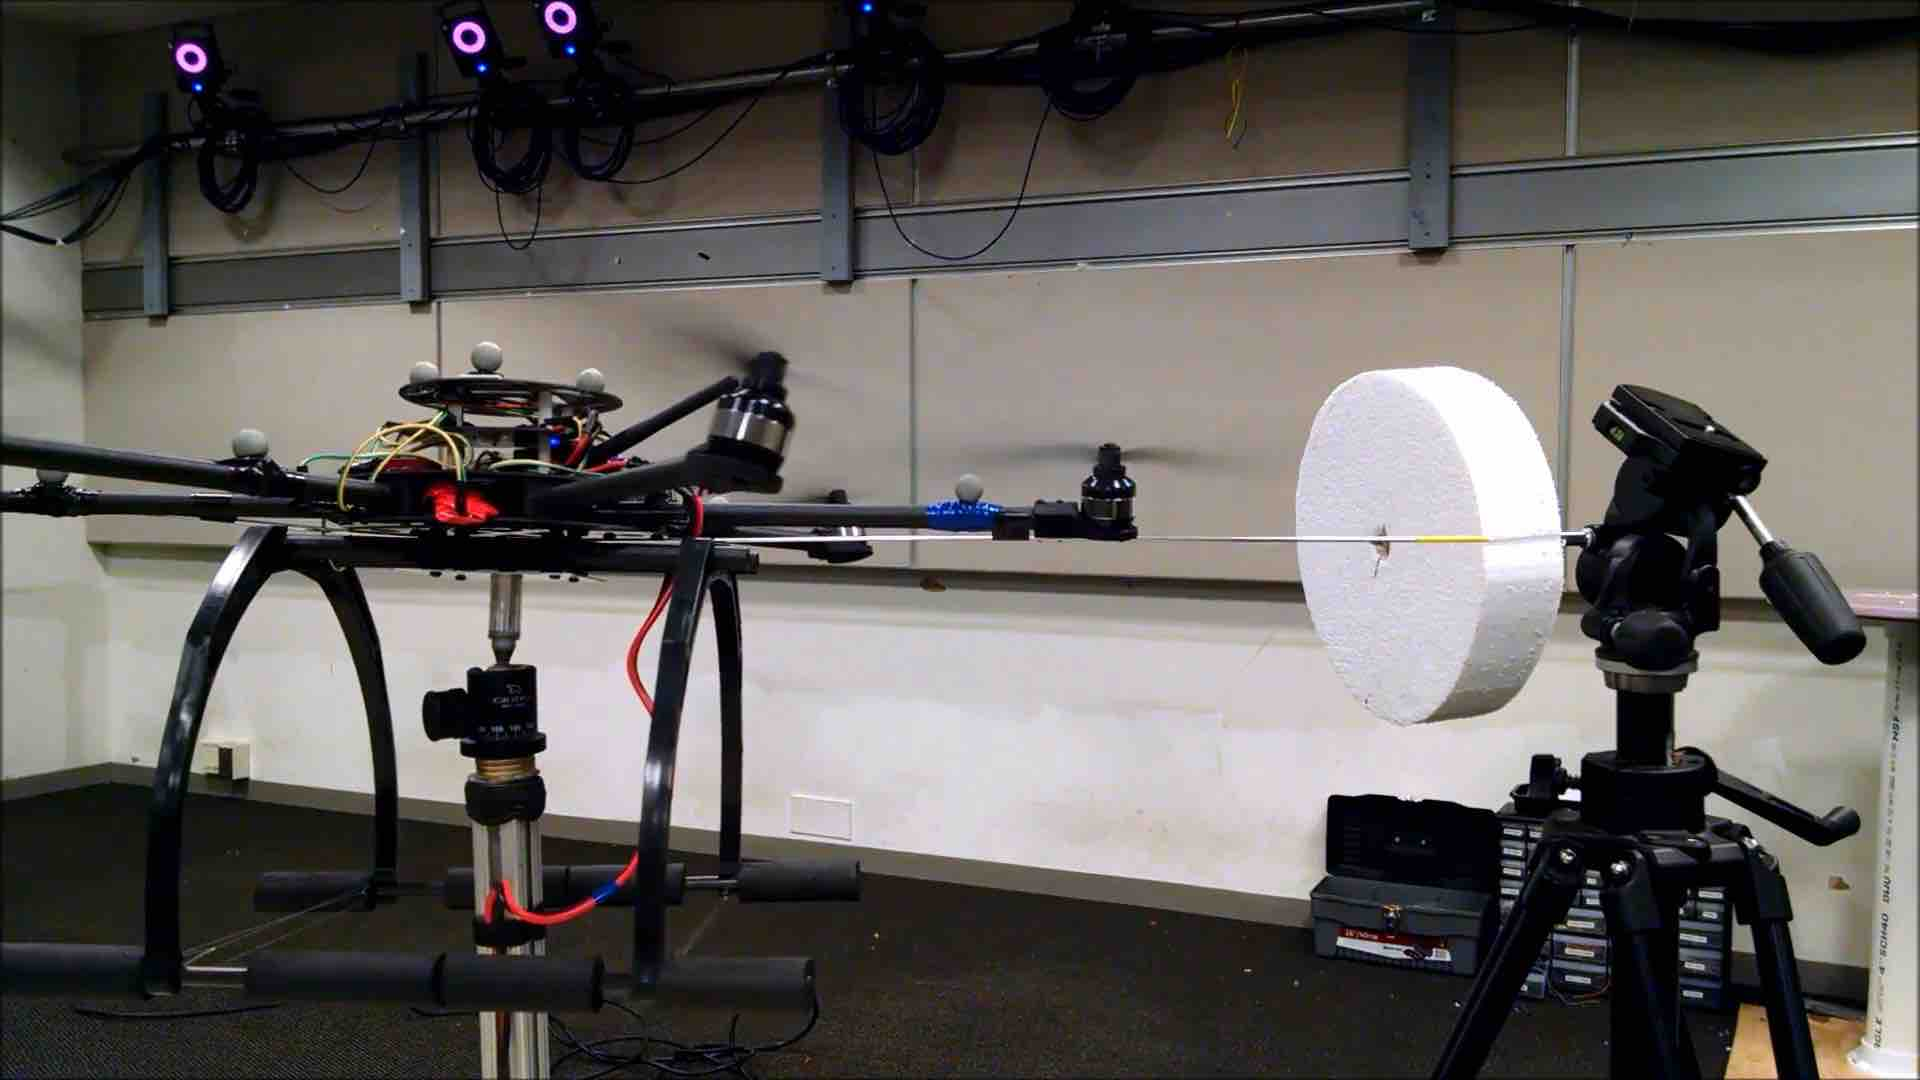
\includegraphics[height=0.7\textheight]{figures/2016_IJCAS/hexrotor}}
\end{center}
\end{frame}   %-----------------------------%



% shape reconstruction
% !TEX root = ../../defense.tex

\section{Shape Reconstruction}
\begin{frame}{Asteroid Shape Modeling}
    \begin{itemize}
        \item<1-> Ground radar used to compute the 3D shape of the asteroid
        \begin{itemize}
            \item Computationally intensive estimation algorithm completed on the ground 
            \item The result is still coarse and only an approximation solution
            \item Not accurate enough for low altitude or landing operations
        \end{itemize}
    \item<2-> Estimating the asteroid shape is the first step of any mission
    \begin{itemize}
        \item Months or years are devoted solely to mapping the surface
        \item Laser ranging used to accurately measure relative distance 
        \item All data is sent to the ground for processing (time and manpower intensive)
    \end{itemize}
    \end{itemize}
    
    \onslide<3->{
        \begin{block}{}
            \begin{center}
                Real-time on board shape estimation
            \end{center}
        \end{block}
    }
\end{frame}

\section[Problem Statement]{Math Background}
\begin{frame}{Problem Statement}
\begin{enumerate}
    \item<1-> Compute the surface shape from range measurements
        \begin{itemize}
            \item Real time and incrementally build the shape
        \end{itemize}
    \item<2-> Utilize shape model in dynamics and controller
        \begin{itemize}
            \item Coupled equations of motion 
            \item Nonlinear controller for maneuvering and landing
        \end{itemize}
    \item<3-> Autonomously navigate around asteroid 
        \begin{itemize}
            \item Locate areas of poor knowledge for measurement
            \item Avoid obstacles or hazards
        \end{itemize}
\end{enumerate}
\end{frame}

\begin{frame}{LIDAR Measurements }
    \begin{itemize}
        \item<1-> Laser pulse used to measure relative distance to surface
        \item<1-> Accurate timing gives the round trip time of flight
            \begin{align*}
                d = \frac{\Delta t}{2 c}
            \end{align*}
    \end{itemize}
     
    \begin{center}
        \only<1>{
            \resizebox{!}{0.6\textheight}{
                \tikzsetnextfilename{laser_range_finder}
\begin{tikzpicture}[
    block/.style={rectangle,thick,
        draw=blue!50,
        fill=blue!20, 
        rounded corners, 
        text centered, 
        minimum height = 3em, 
        minimum width=6em},
        on grid=false,
        node distance=3em,
        auto,
    ]

    \node [block] (detector) {Detector};
    \node [block, below = of detector] (amplifier) {Amplifier};
    \node [block, right = of amplifier] (transmitter) {Transmitter};
    \node [block, below = of $(amplifier)!0.5!(transmitter)$] (timer)  {Clock};
    \node [block, right = of detector] (beamsplitter) {Optics};
    \node [block, right = of beamsplitter] (target) {Target};
    
    \node [below = of timer] (system) {};

    \draw[-Latex] (amplifier) |- node[left] {\scriptsize Stop pulse}  (timer.west);
    \draw[-Latex] (transmitter.south) |- node[right] {\scriptsize Start pulse} (timer.east);
    \draw[-Latex] (detector.south) -- (amplifier.north);

    \draw[-Latex] (transmitter.north) -- (beamsplitter.south);
    \draw[->,decorate,
        decoration={snake,amplitude=.4mm,segment length=2mm,post length=1mm}] (beamsplitter.350) -- (target.190);
    \draw[->,decorate,
        decoration={snake,amplitude=.4mm,segment length=2mm,post length=1mm}] (target.170) -- (beamsplitter.10);

    \draw[-Latex] (beamsplitter) -- (detector);
    \draw[-Latex] (timer) -- node[left] {\scriptsize $\Delta t$} (system);
\end{tikzpicture}

            }
        }
        \only<2>{
            \tikzsetnextfilename{frustrum}
\begin{tikzpicture}[scale=1.7]

    \pgfmathsetmacro{\posalongpath}{0.37}
    \pgfmathsetmacro{\distance}{6};
    \pgfmathsetmacro{\nearplane}{0.37};
    \pgfmathsetmacro{\hfov}{15};
    \pgfmathsetmacro{\wfov}{15};
    \pgfmathsetmacro{\H}{\distance*tan(\hfov/2)};
    \pgfmathsetmacro{\W}{\distance*tan(\wfov/2)};
    \pgfmathsetmacro{\dlength}{1};

    \pgfmathsetmacro{\conex}{1};
    \pgfmathsetmacro{\coney}{0};
    \pgfmathsetmacro{\conez}{0};

    \pgfmathsetmacro{\ctwox}{0};
    \pgfmathsetmacro{\ctwoy}{1};
    \pgfmathsetmacro{\ctwoz}{0};

    \pgfmathsetmacro{\cthreex}{0};
    \pgfmathsetmacro{\cthreey}{0};
    \pgfmathsetmacro{\cthreez}{1};
    
    \coordinate (V) at (0,0,0);
    \coordinate (A) at ($ (\distance * \conex, \distance * \coney, \distance * \conez) + (-\W * \ctwox, -\W * \ctwoy, -\W * \ctwoz) + ( \H * \cthreex, \H * \cthreey, \H * \cthreez) $);
    \coordinate (B) at ($ (\distance * \conex, \distance * \coney, \distance * \conez) + (\W * \ctwox, \W * \ctwoy, \W * \ctwoz) + ( \H * \cthreex, \H * \cthreey, \H * \cthreez) $);
    \coordinate (C) at ($ (\distance * \conex, \distance * \coney, \distance * \conez) + (\W * \ctwox, \W * \ctwoy, \W * \ctwoz) + ( -\H * \cthreex, -\H * \cthreey, -\H * \cthreez) $);
    \coordinate (D) at ($ (\distance * \conex, \distance * \coney, \distance * \conez) + (-\W * \ctwox, -\W * \ctwoy, -\W * \ctwoz) + ( -\H * \cthreex, -\H * \cthreey, -\H * \cthreez) $);

    \coordinate (m1) at ($ (V) + (\dlength * \conex, \dlength * \coney, \dlength * \ctwoz )$);
    \coordinate (m2) at ($ (V) - (\dlength * \conex, \dlength * \coney, \dlength * \ctwoz )$);

    \path (A) -- (V) coordinate[pos=\posalongpath] (A-V);
    \path (B) -- (V) coordinate[pos=\posalongpath] (B-V);
    \path (C) -- (V) coordinate[pos=\posalongpath] (C-V);
    \path (D) -- (V) coordinate[pos=\posalongpath] (D-V);
    
    % labels of points
    \node[below] at (A) {$A$};
    \node[above] at (B) {$B$};
    \node[above] at (C) {$C$};
    \node[right] at (D) {$D$};

    \draw[red!50!black, dashed] (V) -- (A-V) (V) -- (B-V) (V) -- (C-V) (V) -- (D-V);
    % \draw[red!50!black] (A) -- (A-V) (B) -- (B-V) (C) -- (C-V) (D) -- (D-V);
    \draw[red!50!black, -Latex] (A-V) -- (A);
    \draw[red!50!black, -Latex] (B-V) -- (B);
    \draw[red!50!black, -Latex] (C-V) -- (C);
    \draw[red!50!black, -Latex] (D-V) -- (D);
    \fill[red,opacity=0.5,draw=red!80!black,thick] (A) -- (B) -- (C) -- (D) -- cycle;
    \fill[blue,opacity=0.5,draw=blue!80!black,thick] (A-V) -- (B-V) -- (C-V) -- (D-V) -- cycle; 
    
    \draw[blue!50!black, ultra thick] (m1) -- (m2);
    \shade[ball color=blue] (m1) circle (0.2);
    \shade[ball color=blue] (m2) circle (0.2);

\end{tikzpicture}

        }
        \only<3>{
            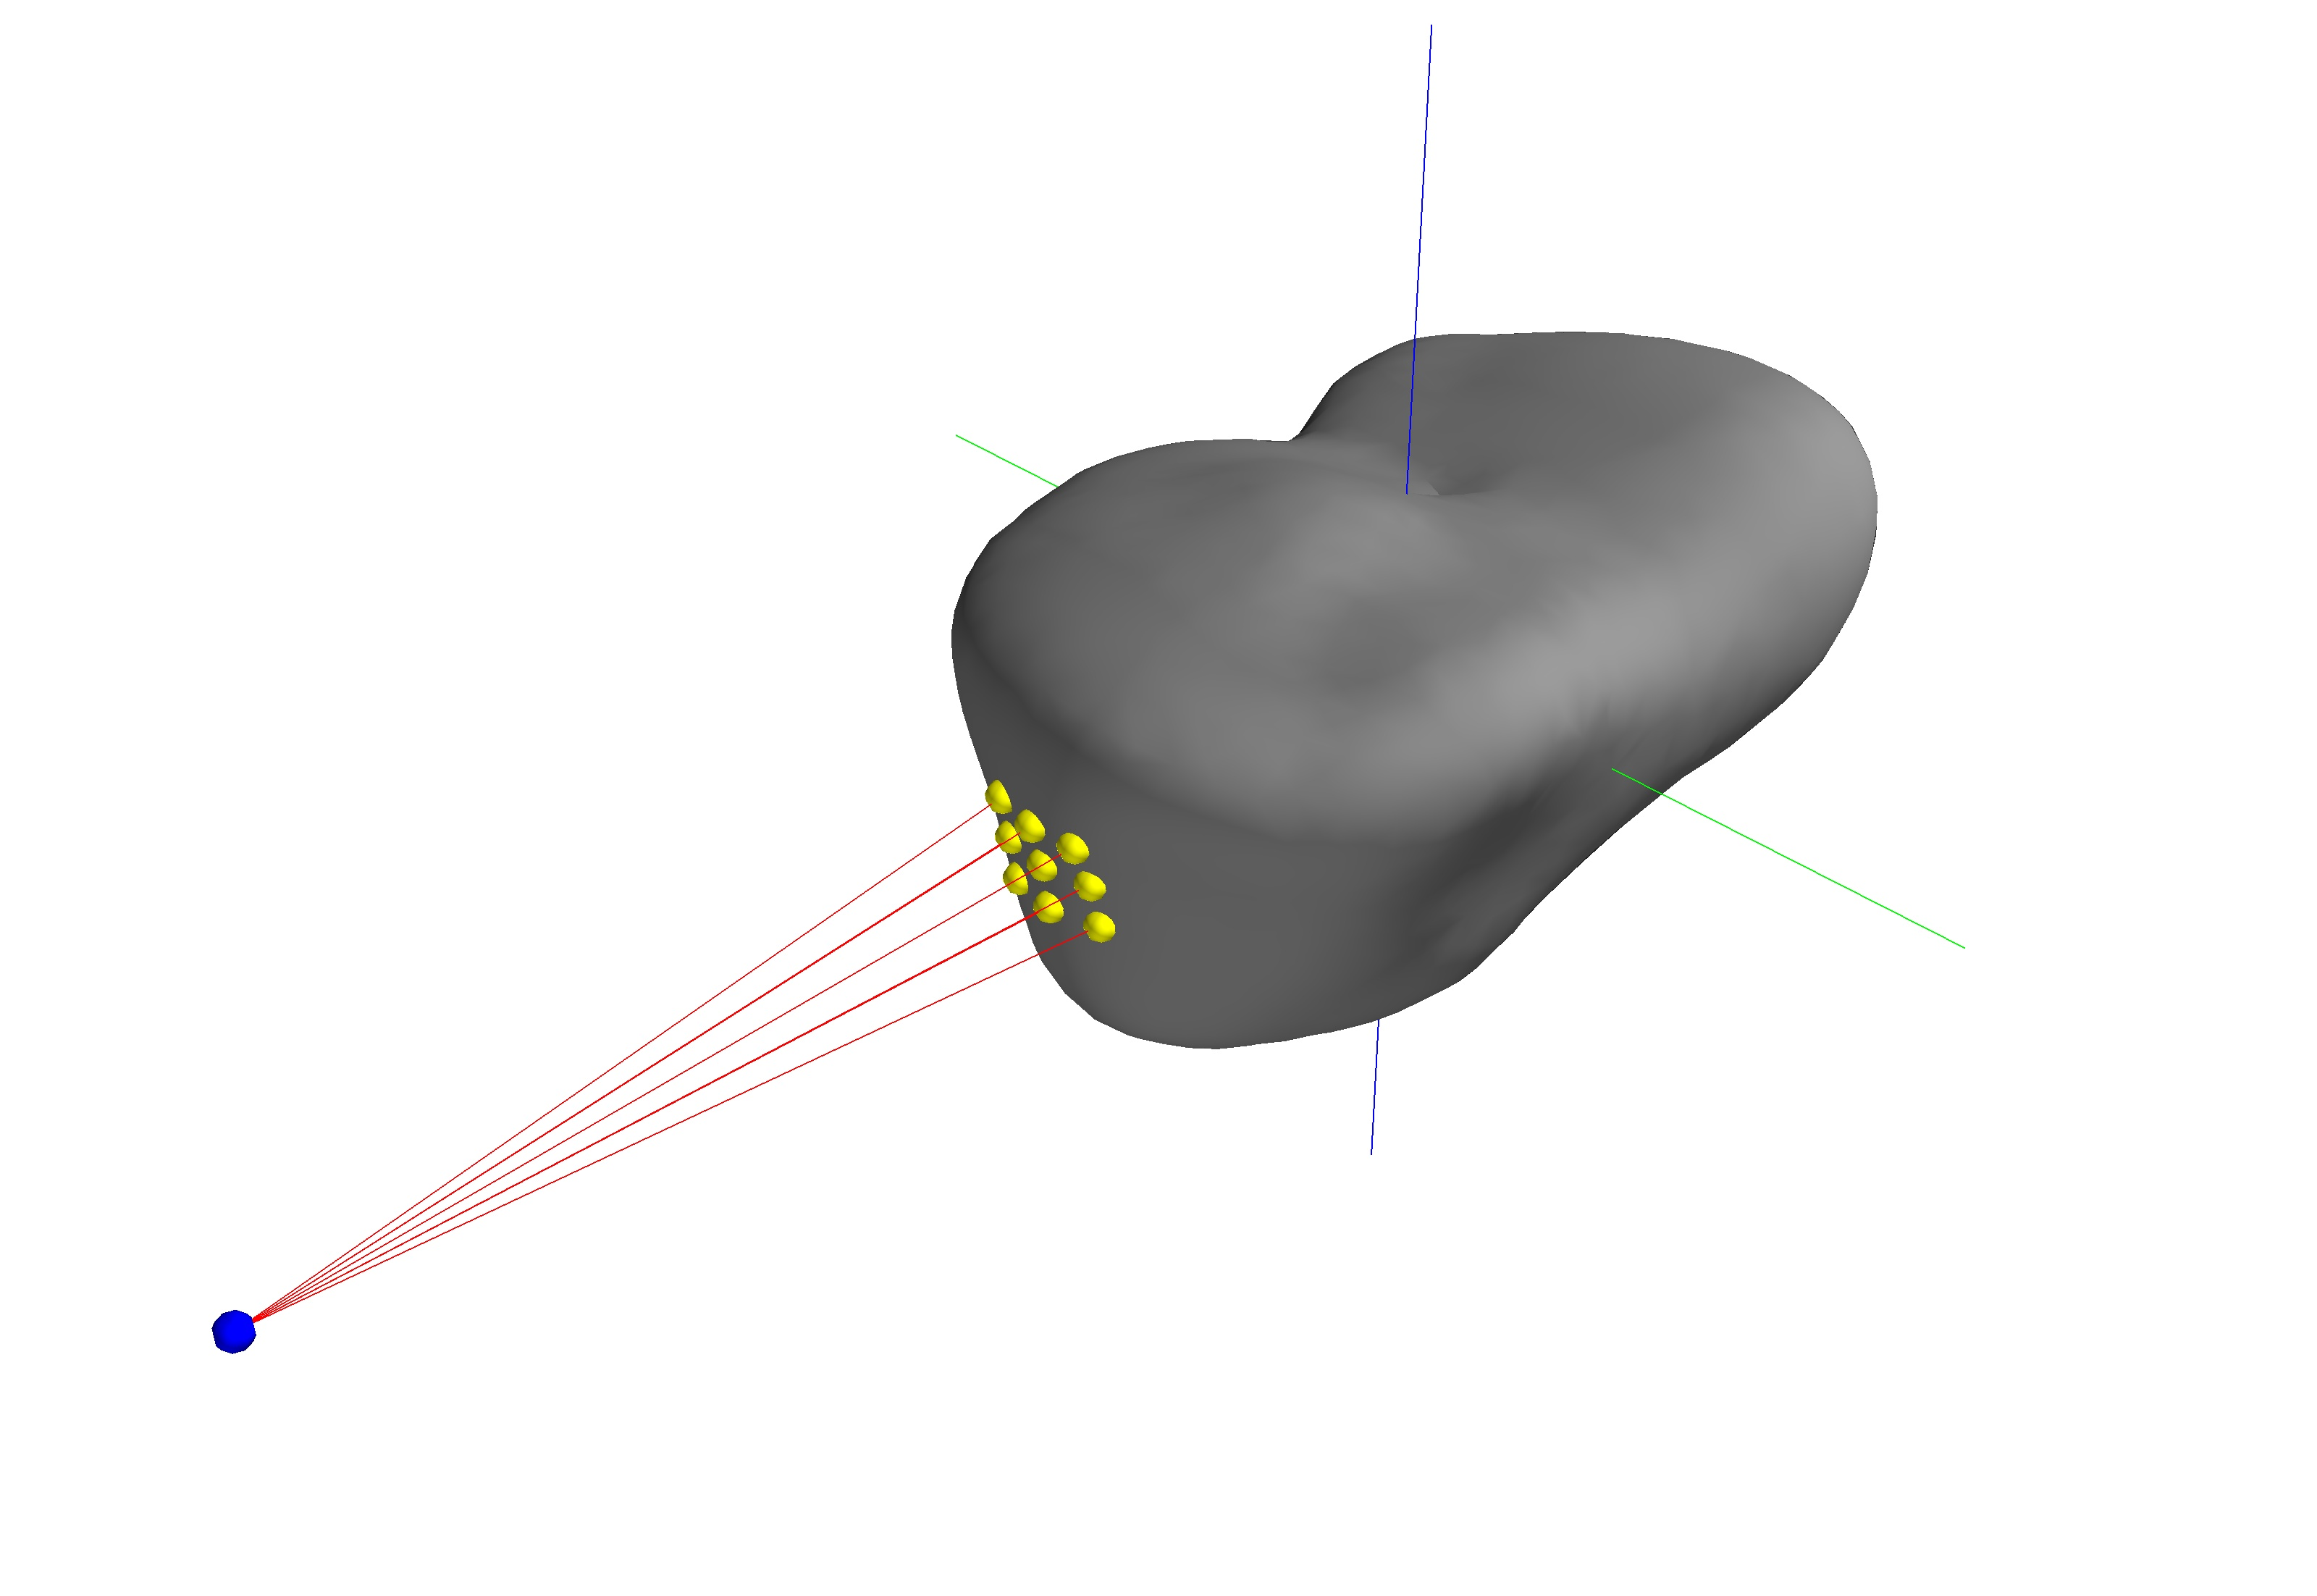
\includegraphics[width=0.75\textwidth,height=0.7\textheight,keepaspectratio]{figures/2018_SSPI/castalia_raycasting_plot.jpg}
        }
    \end{center}
\end{frame}

\begin{frame}{Bayesian Shape Reconstruction}
    \begin{itemize}
        \item<1-> Framework for combining prior and new data 
            \begin{itemize}
                \item Each vertex has an uncertainty -- \( w_i\) in the radial distance
                \item Each measurement contains error -- \( w_{j, i} \) with respect to each vertex
            \end{itemize}
            \begin{align*}
                v_i \sim \mathcal{N}(r_i, w_i^2) , \quad
                p_{j,i} \sim \mathcal{N}(r_{j,i}, w_{j,i}^2)
            \end{align*}
        \item<2-> New data used to update each vertex and reduce uncertainty
    \begin{align*}\label{eq:posterior_probability}
        \mathcal{N} \parenth{\frac{w_{j, i}^2 r_i + w_i^2 r_{j, i}}{w_i^2 + w_{j, i}^2} , \frac{w_i^2  w_{j, i}^2}{w_i^2 +  w_{j, i}^2}} .
    \end{align*}
    \end{itemize}
\end{frame}

\subsection{Shape Reconstruction}
\begin{frame}{Geographos Reconstruction}
    \begin{itemize}
        \item Potentially hazardous Apollo group asteroid discovered in 1951
    \end{itemize}
    
    \begin{center}
        \includemedia[
        keepaspectratio,
        activate=pagevisible,
        addresource=videos/geographos.mp4,
        flashvars={source=videos/geographos.mp4}
        ]{\includegraphics[trim={20cm 15cm 20cm 15cm},clip,keepaspectratio,width=0.5\textwidth]{figures/computational_geometry/mesh_update/geographos/partial_7489.jpg}}{VPlayer.swf}%
        \includemedia[
        keepaspectratio,
        activate=pagevisible,
        addresource=videos/geographos_weight.mp4,
        flashvars={source=videos/geographos_weight.mp4}
        ]{\includegraphics[trim={20cm 15cm 20cm 15cm},clip,keepaspectratio,width=0.5\textwidth]{figures/computational_geometry/mesh_update/geographos/partial_7489.jpg}}{VPlayer.swf}
\end{center}
\end{frame}

\begin{frame}{Golevka Reconstruction}
    \begin{itemize}
        \item Potentially hazardous Apollo group asteroid discovered in 1995
    \end{itemize}
    \begin{center}
        \includemedia[
        keepaspectratio,
        activate=pagevisible,
        addresource=videos/golevka.mp4,
        flashvars={source=videos/golevka.mp4}
        ]{\includegraphics[trim={20cm 10cm 20cm 10cm},clip,keepaspectratio,width=0.5\textwidth]{figures/computational_geometry/mesh_update/golevka/partial_5285.jpg}}{VPlayer.swf}%
        \includemedia[
        keepaspectratio,
        activate=pagevisible,
        addresource=videos/golevka_weight.mp4,
        flashvars={source=videos/golevka_weight.mp4}
        ]{\includegraphics[trim={20cm 10cm 20cm 10cm},clip,keepaspectratio,width=0.5\textwidth]{figures/computational_geometry/mesh_update/golevka/partial_5285.jpg}}{VPlayer.swf}
\end{center}
\end{frame}

\subsection{Guidance}
\begin{frame}{Optimal Guidance}
    \begin{itemize}
        \item Cost function used to determine future states which provides best measurements
        \item User selected weighting between: uncertainty, distance, and control effort
            \begin{align*}
                J_i (\ipos, \iatt, \aatt) = \alpha_w J_{w_i} + \alpha_d J_{d_i}(\rpos) + \alpha_c J_{c_i}(\rpos)
            \end{align*}
    \end{itemize}

    52760 exploration videos
\end{frame}

\subsection{Refinement}
\begin{frame}{Landing Site Selection}
    \begin{itemize}
        \item The shape estimate provides sufficient detail to determine the surface slope
            \begin{align*}
                \cos \parenth{ \pi - \phi } = \frac{\vc{n}_f \cdot U_m}{\norm{U_m}},
            \end{align*}
        \item The desired landing area selected to minimize: slope and distance
        \item Desired landing area used for multi-resolution refinement
    \end{itemize}
    \begin{center}
        \only<1>{
        \includegraphics[width=0.5\textwidth]{figures/computational_geometry/dynamic_exploration/castalia/refine/slope.pdf}%
        \includegraphics[width=0.5\textwidth,keepaspectratio]{figures/computational_geometry/dynamic_exploration/castalia/refine/slope_masked.pdf}
    }
    \only<2>{
        \includegraphics[width=0.5\textwidth]{figures/computational_geometry/dynamic_exploration/castalia/refine/dist.pdf}%
        \includegraphics[width=0.5\textwidth,keepaspectratio]{figures/computational_geometry/dynamic_exploration/castalia/refine/dist_masked.pdf}
    }
    \only<3>{
        \includegraphics[width=0.5\textwidth]{figures/computational_geometry/dynamic_exploration/castalia/refine/science.pdf}%
        \includegraphics[width=0.5\textwidth,keepaspectratio]{figures/computational_geometry/dynamic_exploration/castalia/refine/science_masked.pdf}
    }
    \only<4>{
        \includegraphics[width=0.5\textwidth]{figures/computational_geometry/dynamic_exploration/castalia/refine/cost.pdf}%
    }
    \end{center}
\end{frame}

\begin{frame}{Multi-resolution refinement}
    \begin{itemize}
        \item The mesh resolution limits the size of captured features
        \item A uniform high resolution mesh would be computationally intractable
    \end{itemize}
    \begin{center}%
        \only<1>{
        \includegraphics[width=0.49\textwidth]{figures/computational_geometry/isotropic/original_cube.jpg}%
        \includegraphics[width=0.49\textwidth]{figures/computational_geometry/isotropic/remesh_cube.jpg}
    }
    \only<2>{
\includegraphics[width=0.5\textwidth]{figures/computational_geometry/dynamic_exploration/castalia/refine/density.pdf}%
\includegraphics[width=0.5\textwidth]{figures/computational_geometry/dynamic_exploration/castalia/land/density.pdf}
    }
    \end{center}
\end{frame}

\begin{frame}{4769 Castalia exploration and landing}
    \begin{center}
        Show exploration, refinement and landing videos
    \end{center}
\end{frame}


% !TEX root = ../../defense.tex
\section{Conclusions}
\begin{frame}{Conclusions}
    \begin{enumerate}
        \item Low thrust transfers for large scale orbital manuevers 
            \pause
            \begin{alertblock}{}
                \begin{itemize}
                    \item Transfers via reachability sets on a \Poincare section
                    \item Examples in 3BP and around 4769 Castalia
                \end{itemize}
            \end{alertblock}
            \pause
        \item Geometric control for close proximity operations
            \pause
            \begin{alertblock}{}
                \begin{itemize}
                    \item Geometric control for precise attitude and state tracking
                    \item Utilized for shape reconstruction and landing
                \end{itemize}
            \end{alertblock}
            \pause
        \item Autonomous shape reconstruction
            \begin{alertblock}{}
                \begin{itemize}
                    \item Bayesian framework for local shape reconstruction
                    \item Examples around several asteroids with landing onto 4769 Castalia
                \end{itemize}
            \end{alertblock}
    \end{enumerate}
\end{frame}


% !TEX root = ../presentation.tex

\begin{frame}[c]{Thank you}
  \centering
  
  \textbf{\large Flight Dynamics \& Control Lab} \\
  Mechanical \& Aerospace Engineering \\
  School of Engineering \& Applied Science
  
  \begin{center} %figure%
        \includegraphics[width=0.75\textwidth]{gw_txh_2cs_pos}
    \end{center}
  
  \url{https://fdcl.seas.gwu.edu}
\end{frame}


% % !TEX Root = ../proposal.tex

\appendix
\section[Appendix]{Appendix}
\subsection[Gravity Models]{Gravitational Modelling}

\begin{frame}[noframenumbering,label=astro] %----------------------------------------------%
\frametitle{Astrodynamics}

\only<1>{
\begin{block}{Newton's Law of Universal Gravitation}
    Any two bodies attract one another with a force proportional to the product of their masses and invesely proportional to the square of the distance between them
    \[
    \vc{F} = - \frac{G m_1 m_2}{ r^2} \frac{\vc{r}}{r}
    \]
\end{block}
}
\only<2>{
\begin{block}{N-Body}
    Gravitational attraction of \( n \) bodies acting on the particle of interest \( m_i \)
    \[
    m_i \ddot{\vc{r}}_i = -G \sum_{\substack{j = 1\\j\neq i}}^n \frac{m_i m_j}{r_{ji}^3} \vc{r}_{ji}
    \]
    Motion of \( \bar{r}_j (t) \) is not known - Not solvable in general
    
\end{block}
}
\hyperlink{slide:system_model_challenges}{\beamergotobutton{Dynamic Challenges}}
\end{frame} %--------------------------------------------------------------%

\begin{frame}[noframenumbering,label=centrobaric]
\frametitle{Gravitational Modeling}
\begin{block}{Centrobaric Body}
    \( \vc{F} = -\frac{G m_1 m_2}{R^2} \vc{a}_1 \) for all particles outside of body
\end{block}

\begin{columns}
    \begin{column}{0.5\textwidth}
        \begin{itemize}
            \item<2-> Only applies to spherically symmetric bodies 
            \item<3-> \Emph{Gravity Model} requires accurate tracking of SC
                \begin{itemize}
                    \item Spherical Harmonic
                    \item Mass concentration
                    \item Polyhedron Potential
                \end{itemize}
        \end{itemize}
    \end{column}
    \begin{column}{0.5\textwidth}
        \visible<2->{
            \includegraphics[width=\textwidth,height=0.5\textheight,keepaspectratio]{figures/defense/earth_layers.jpg}
        }
    \end{column}
\end{columns}

\note[itemize]{
    \item Models require detailed data from orbit about asteroid (OD process determines gravity field)
    \item Simplified models (triaxial ellipsoid allows analytical insight)
    \item Previous work fails to consider coupled dyanmics
    }
\end{frame}

\begin{frame}[noframenumbering]{Polyhedron Gravitation Model}
\label{slide:polyhedron_gravity}
\begin{itemize}
    \item Potential is a function of only the shape model
    \item Globally valid, closed-form expression of potential
    \item Exact potential assumes a constant density 
    \item Accuracy solely dependent on shape model
\end{itemize}
\only<2>{
\begin{align*}\label{eq:potential}
    U(\vc{r}) &= \frac{1}{2} G \sigma \sum_{e \in \text{edges}} \vc{r}_e \cdot \vc{E}_e \cdot \vc{r}_e \cdot L_e - \frac{1}{2}G \sigma \sum_{f \in \text{faces}} \vc{r}_f \cdot \vc{F}_f \cdot \vc{r}_f \cdot \omega_f 
\end{align*}
}
\only<3>{
\begin{center}
  % \animategraphics[controls,autoplay,loop,width=0.5\textwidth]{30}{animation/2016AAS/castalia/IMG}{00001}{00999}~\hfill
  % \includegraphics[width=0.5\textwidth]{figures/2016AAS/radius_contour.pdf}
\end{center}
}
\hyperlink{slide:asteroid_transfer}{\beamergotobutton{Asteroid Transfer}}
\end{frame}

\begin{frame}[noframenumbering]{Astrodynamics}%-------------------------------------------------------%
\label{slide:astrodynamics}

\only<1>{
\begin{block}{Integrals of Motion}
    Require \( 6 n \) integrals of motion but know \( 10 \)
        \begin{itemize}
            \item Linear Momentum - system CM constant speed - \( 6 \) constants
            \item Angular Momentum - system angular moment - \( 3 \) constants
            \item Total Energy - Conservative system - \( 1 \) constant
        \end{itemize}
    Even two-body problem is not solvable
\end{block}
}
\only<2>{
\begin{block}{Relative Motion}
Really care about relative motion of \( m_i \) wrt \( m_q \)
\[
    \ddot{\vc{r}}_{qi} + G \frac{m_i + m_q}{r_{qi}^3} \vc{r}_{qi} = G \sum_{\substack{j = 1\\j\neq i,q}}^n m_j \parenth{ \frac{\vc{r}_{ij}}{r_{ij}^3} - \frac{\vc{r}_{qj}}{r_{qj}^3}} \vc{r}_{ji}
\]
\end{block}
}

\end{frame} %----------------------------------------------------------% 

\subsection{Attitude Coupling}

\begin{frame}[noframenumbering,label=grav] %---------------------------------------%
\frametitle{Gravity Expansion}
\only<1>{
\begin{block}{Force due to gravity on body \( B\) from particle \( P \)}
\begin{equation*}
    \vc{F} = -G m_P \int_{\mathcal{B}} \vc{r} \parenth{r^2}^{-\frac{3}{2}} \, d m
\end{equation*}
\end{block}
}
\only<2>{
\begin{block}{Binomial Expansion}

\begin{align*}
    \vc{F} &= - \frac{G m_P m_B}{R^2} \parenth{\vc{a}_1 + \sum_{i=2}^\infty \vc{f}^{(i)}} \\
    \vc{f}^{(2)} &= \frac{1}{m_B R^2} \braces{\frac{3}{2} \bracket{ \tr{J_B} - 5 \vc{a}_1 \cdot J_B \cdot \vc{a}_1} \vc{a}_1 + 3 J_B \cdot \vc{a}_1}
\end{align*}
\end{block}
}
\only<3>{
\begin{block}{Gravity Moment}
\begin{equation*}
    \vc{M} = \frac{3 G m_B}{R^3} \vc{a}_1 \times J \cdot \vc{a}_1 + \frac{G m_B m_P}{R} \sum_{i=3}^\infty \vc{a}_1 \times \vc{f}^{(i)}
\end{equation*}
%\begin{center}
%CG \( \neq \) CM 
%\end{center}
\end{block}
}

\end{frame}%-------------------------------------------------------------%


%\begin{frame}[noframenumbering,label=srp]{Solar Radiation Pressure} %---------------------------------------------------%

%\begin{block}{Constant Area Approximation}
%Momentum transfer from solar photons striking spacecraft
%\begin{align*}
%    \vc{a}_{SRP} = - \frac{\parenth{1 + \rho} P_0 A_{S}}{M_S} \frac{\vc{d} - \vc{r}}{\norm{\vc{d}-\vc{r}}^3}
%\end{align*}

%\( P_0\) is a solar flux constant \SI{1e8}{\kilogram\kilo\meter\cubed\per\second\squared\per\meter\squared}

%\( B_S = \frac{M_S}{A_S} \) is a mass to area ratio - \( 20 - 40 \, \si{\kilogram\per\meter\squared} \)

%\( \rho \) is total reflectance or albedo of body

%\( \vc{d}, \vc{r} \) defined in small body frame to Sun and S/C respectively
%\end{block}
%\begin{itemize}
%    \item Large bodies, i.e. 433 Eros, SRP may be neglected
%    \item Small bodies, \( < 1-5 \si{\kilo\meter} \), SRP is crucial
%\end{itemize}
%\end{frame} %-----------------------------------------------------------%

%\subsection{Dynamics}

%\begin{frame}[noframenumbering]{Lagrange's Equations}%---------------------------------------------%
%\label{slide:lagrange}
%\begin{block}{Conservative System}
%  All applied forces \( \vc{F}_i \) are derivable from a potential function \( V(x_1, x_2, \ldots, x_{3N}) \) : \(\vc{F}_i = -\deriv{V}{\vc{x}_i}\)
%\end{block}

%\only<1>{
%\begin{block}{Hamilton's Principle}
%    The actual path in configuration space followed by a holonomic system during the fixed interval \( t_0 \) to \( t_1\) is such that the action integral:
%    \[
%    S = \int_{t_0}^{t_1} L(q, \dot{q}) dt
%    \]
%    is stationary with respect to path variations which vanish at the end-points.
%\end{block}
%}
%\only<2>{
%\begin{block}{Variation of action integral}
%\begin{align*}
%    \delta S &= \int_{t_0}^{t_1} \deriv{L}{q} \delta q + \deriv{L}{\dot{q}} \delta \dot{q} \, dt \\
%        &= \int_{t_0}^{t_1} \deriv{L}{q} \delta q - \frac{d}{dt} \left( \deriv{L}{\dot{q}}\right) \delta q \, dt - \left. \left[ \deriv{L}{\dot{q}} \delta q\right] \right|_0^T \\
%    &= \int_{t_0}^{t_1} \deriv{L}{q} - \frac{d}{dt} \left( \deriv{L}{\dot{q}}   \right) \, dt \, ,
%\end{align*}
%\end{block}
%}
%\end{frame}%---------------------------------------------------------------------------%

%\begin{frame}[noframenumbering]{Jacobi Integral}
%\label{slide:jacobi}
%\only<1>{
%\begin{block}{Total Mechanical Energy}
%\begin{enumerate}
%    \item Generalized force from potential function: \( Q_i = -\deriv{V}{q_i} \)
%    \item Work is path independent: \( W = \sum_{i=1}^{n} \int_{A_i}^{B_i} Q_i \, dq_i \)
%\end{enumerate}

%    If no other forces do work, then total mechanical energy is conserved:  \(  E(q, \dot{q}) = T + V   \)
%\end{block}
%}
%\only<2>{
%\begin{block}{More general constant}
%\begin{enumerate}
%    \item Standard Form of Lagrange's equation applies
%    \item Lagrangian is not explicit fcn of time
%    \item Constraints may be expressed: \( \sum_{i=1}^n a_{ji} d q_i = 0\)
%\end{enumerate}

%\[
%    h = \sum_{i=1}^n \deriv{L}{\dot{q}_i} \dot{q}_i - L 
%\]
%\end{block}
%}

%\end{frame} %-----------------------------------------------------------%

%\begin{frame}[noframenumbering] %------------------------------------%
%\frametitle{Variational Principle}
%    \begin{itemize}
%        \item Variational Integrators
%            \begin{itemize}
%                \item Structure-preserving integrators for Hamiltonian systems
%                \item Obtained by discretizing variational principle
%            \end{itemize}
%    \end{itemize}
%    \pause
%    \begin{columns}[c]
%        \begin{column}{0.5\textwidth}
%            \centering
%            \begin{beamercolorbox}[wd=0.8\columnwidth,sep=0.05cm,center]{numerical} Continuous Time \end{beamercolorbox}
%            \begin{beamercolorbox}[wd=0.8\columnwidth,sep=0.05cm,center]{numerical} 
%                Configuration Space \\
%                \( \parenth{q, \dot{q} } \in TQ \)
%            \end{beamercolorbox}
%            \begin{beamercolorbox}[wd=0.8\columnwidth,sep=0.05cm,center]{numerical} 
%                Lagrangian \\
%                \( L\parenth{q, \dot{q} } \)
%            \end{beamercolorbox}
%            \begin{beamercolorbox}[wd=0.8\columnwidth,sep=0.05cm,center]{numerical} 
%                Action Integral \\
%                \( S = \int_{0}^T L\left( q, \dot{q}\right) \, dt \)
%            \end{beamercolorbox}
%            \begin{beamercolorbox}[wd=0.8\columnwidth,sep=0.05cm,center]{numerical} 
%                Stationary Action \\
%                \( \delta S = 0 \)
%            \end{beamercolorbox}
%%           \begin{beamercolorbox}[wd=0.8\columnwidth,sep=0.05cm,center]{numerical} 
%%               Legendre Transform \\
%%               \( p_i = \deriv{L}{\dot{q}} \)
%%           \end{beamercolorbox}
%            \begin{beamercolorbox}[wd=0.8\columnwidth,sep=0.05cm,center]{numerical} 
%                Equation of Motion \\
%                \( \ddot{q} = f \parenth{q, \dot{q} } \)
%            \end{beamercolorbox}
%        \end{column}
%        \pause
%        \begin{column}{0.5\textwidth}
%            \centering
%            \begin{beamercolorbox}[wd=0.8\columnwidth,sep=0.05cm,center]{numerical} Discrete Time \end{beamercolorbox}
%            \begin{beamercolorbox}[wd=0.8\columnwidth,sep=0.05cm,center]{numerical} 
%                Configuration Space \\
%                \( \parenth{q_k, q_{k+1} } \in Q \times Q \)
%            \end{beamercolorbox}
%            \begin{beamercolorbox}[wd=0.8\columnwidth,sep=0.05cm,center]{numerical} 
%                Lagrangian \\
%                \( L_d\parenth{q_k, q_{k+1}} \)
%            \end{beamercolorbox}
%            \begin{beamercolorbox}[wd=0.8\columnwidth,sep=0.05cm,center]{numerical} 
%                Action Sum \\
%                \( S_d = \sum_{k=0}^{N-1} L_d(q_k, q_{k+1}) \)
%            \end{beamercolorbox}
%            \begin{beamercolorbox}[wd=0.8\columnwidth,sep=0.05cm,center]{numerical} 
%                Stationary Action \\
%                \( \delta S_d = 0 \)
%            \end{beamercolorbox}
%%           \begin{beamercolorbox}[wd=0.8\columnwidth,sep=0.05cm,center]{numerical} 
%%               Fiber Derivative \\
%%               \( p_k = - \deriv{L_d(q_k, q_{k+1})}{q_k} \) \\
%%               \( p_{k+1} = \deriv{L_d(q_k, q_{k+1})}{q_{k+1}} \)
%%           \end{beamercolorbox}
%            \begin{beamercolorbox}[wd=0.8\columnwidth,sep=0.05cm,center]{numerical} 
%                Equation of Motion \\
%                \( q_{k+2} = f_d \parenth{q_k, q_{k+1} } \)
%            \end{beamercolorbox}
%        \end{column}
%    \end{columns}
    
%    \note[itemize]{
%        \item Continous time - discretization occurs at end while implemented in digital computer
%        \item Discrete time - discretization occurs at the beginning. 
%        Dynamics derived in discrete time
%        \item Legendre transform allows for expression of dynamics in Hamiltonian form
%    }
%\end{frame}%-----------------------------------------%

%\begin{frame}[t,noframenumbering]{Dynamics of Rigid Body} %------------------------------------------------%
%    \begin{block}{Newton's Law}
        
%        \begin{align*}
%            F_x &= m \parenth{\dot{v}_x + v_z \omega_y - v_y \omega_z} \\
%            F_y &= m \parenth{\dot{v}_y + v_x \omega_z - v_z \omega_x} \\
%            F_z &= m \parenth{\dot{v}_z + v_y \omega_x - v_x \omega_y} \\
%        \end{align*}
%    \end{block}
    
%    \begin{block}{Euler's Law}
%        \begin{align*}
%            {M}_x &= I_{xx} \dot{\omega}_x + \parenth{I_{zz}-I_{yy}} \omega_y \omega_z \\
%            {M}_y &= I_{yy} \dot{\omega}_y + \parenth{I_{xx}-I_{zz}} \omega_z \omega_x \\
%            {M}_z &= I_{zz} \dot{\omega}_z + \parenth{I_{yy}-I_{xx}} \omega_x \omega_y \\
%        \end{align*}
%    \end{block}
%\end{frame} %----------------------------------------------------------------------%

%\begin{frame}[noframenumbering]{Spacecraft Propulsion}\label{slide:propulsion}%------------------------------------------------%
%\begin{block}{Ideal Rocket Equation}
%    Amount of propellant required for a given velocity change
%    \[
%        \Delta V = - g_0 I_{sp} \ln\parenth{\frac{m_f}{m_i}}
%    \]
%\end{block}

%\begin{itemize}
%    \item High exhaust speeds make electric propulsion attractive
%    \item Much higher efficiency than chemical propulsion
%\end{itemize}
%\hyperlink{slide:lowthrust_vehicles}{\beamergotobutton{Low-Thrust Vehicles}}

%\end{frame} %----------------------------------------------------------------%

%% Differences when considering an asteroid - polyhedron model

%\subsection{Attitude Kinematics}
%\begin{frame}[noframenumbering]{Attitude Kinematics}
%\label{slide:attitude_kinematics}

%\begin{columns}
%\begin{column}{0.5\textwidth}
%\begin{itemize}
%    \item Many ways to represent the orientation of a rigid body
%    \begin{itemize}
%        \item Conceptual simplicity
%        \item Computational considerations
%        \item Legacy hardware/code
%        \item Mathmatical simplicity/convience
%    \end{itemize}
%\end{itemize}
%\end{column}
%\pause
%\begin{column}{0.5\textwidth}
%    \begin{itemize}
%        \item Euler axis and angle (4)
%        \item Rotation Matrix (9)
%        \item Euler angles (3)
%        \item Quaternion (4)
%        \item Rodriguez Parameters (4)
%        \item Modified Rodriguez parameters (4)
%    \end{itemize}
%\end{column}
%\end{columns}
%\pause
%\begin{block}{Minimal Representations}
%    All minimal attitude representations have kinematic singularities and are not suitable for large rotations.
%\end{block}

%\hyperlink{slide:attitude_control}{\beamergotobutton{Attitude Control}}
%\end{frame}

%\begin{frame}[noframenumbering]{Attitude Parameterizations}
%\label{slide:attitude_parameterizations}
%    \begin{itemize}
%        \item Euler Angles
%        \begin{itemize}
%            \item Minimal representation used for small attitude changes.
%            \item Singularities exist for large angle slews: requires switching between 24 sequences
%            \item Complicated trigonometric functions
%        \end{itemize}
%        \pause
%        \vs
%        \item Quaternion 
%        \begin{itemize}
%            \item No singularities
%            \item Two anti-podal quaternions for the same attitude
%            \item Unwinding behavior for control systems
%        \end{itemize}
%        \pause
%        \vs
%        \item Geometric control
%        \begin{itemize}
%            \item Globally and uniquely characterize attitude: \( R \in \SO \)
%            \item Controller is globally valid for large angle maneuvers
%        \end{itemize}
%    \end{itemize}

%\end{frame}

%\begin{frame}[t,noframenumbering]\frametitle{Constrained Attitude Control}
%\label{slide:attitude_constraints}
%    \begin{itemize}
%    \item \Emph{Constrained attitude control} : reorient vehicle while avoiding pointing at obstacles
%    \begin{itemize}
%        \item Exclusion zones for payloads e.g infrared telescope
%        \item UAVs manuevering in congested locations
%        \item Laser/Radio emitters on spacecraft
%    \end{itemize}
%    \pause
%    \vs
%    \item Previous approaches have several issues
%    \begin{itemize}
%        \item Attitude parameterizations: singularities/ambiguities
%        \item Ad-hoc path planning: difficult to generalize to arbitrary obstacles
%        \item Randomized methods: lack of stability guarantees
%        \item Optimization based: expensive to compute and only provides open-loop control  
%    \end{itemize}
%\end{itemize}


%\end{frame}


\end{document}

